% SPDX-FileCopyrightText: 2026 Hasan Melih Akbulut
% SPDX-License-Identifier: CC-BY-4.0
%
% The thesis: a design description of the neuromorphic space SoC.
%
%   make            -> main.pdf   (tectonic, or pdflatex+bibtex)
%
% Chapters live in chapters/ and are written one per file so that they
% can be worked on independently; figures/ carries the generated PDFs
% and the scripts that generate them, so that every picture in this
% document can be reproduced from the run trees it was drawn from.

\documentclass[11pt,a4paper,oneside]{report}

\usepackage[T1]{fontenc}
\usepackage[utf8]{inputenc}
\usepackage{lmodern}
\usepackage{upgreek}
\usepackage{microtype}
\usepackage[a4paper,margin=2.4cm,bottom=2.8cm]{geometry}

\usepackage{graphicx}
\usepackage{booktabs}
\usepackage{longtable}
\usepackage{tabularx}
\usepackage{array}
\usepackage{multirow}
\usepackage{siunitx}
\usepackage[dvipsnames,table]{xcolor}
\usepackage{tikz}
\usetikzlibrary{shapes.geometric,arrows.meta,positioning,fit,calc,backgrounds}
\usepackage{caption}
\usepackage{subcaption}
\usepackage{amsmath}
\usepackage{listings}
\usepackage{csquotes}
\usepackage{fancyhdr}
\usepackage[hidelinks,breaklinks]{hyperref}
\usepackage[nameinlink]{cleveref}

% ---- house style ----------------------------------------------------
\definecolor{accent}{HTML}{0072B2}
\definecolor{rule}{HTML}{555555}
\hypersetup{colorlinks=true,linkcolor=accent,citecolor=accent,urlcolor=accent}

\newcommand{\code}[1]{{\small\texttt{#1}}}
% \dcite{63}{section 8.4} -> docs/63 section 8.4
\newcommand{\dcite}[2]{\mbox{\code{docs/#1}\,#2}}
\newcommand{\fact}{\textsuperscript{[fact]}}

% group-digits=integer IS NOT OPTIONAL HERE. Without it siunitx
% groups the DECIMAL part too, and this document's most-quoted
% numbers have four decimal places: the worst setup slack printed
% as 7.575,8 ns and the hold margin as 0.029,6 ns in two published
% revisions, 44 numbers in all.
\sisetup{detect-all,group-separator={,},group-minimum-digits=4,
         group-digits=integer}
% THE MICRO SIGN. Under T1 with lmodern, siunitx's own \micro prefix
% prints a t-cedilla: two revisions of this document shipped a
% "700.08 tm" standard-cell channel. siunitx's text-micro and
% math-micro keys do not fix it -- they were tried, and the glyph does
% not change -- so the unit is declared here instead, with upgreek's
% upright mu, and every unit in the text uses \um rather than the
% built-in prefix and metre.
\DeclareSIUnit{\um}{\text{\ensuremath{\upmu}}m}

\captionsetup{font=small,labelfont=bf,width=0.94\linewidth}
\setlength{\parskip}{0.35em}
\setlength{\parindent}{0pt}

\lstset{basicstyle=\ttfamily\footnotesize,breaklines=true,frame=single,
        rulecolor=\color{rule},framesep=4pt,columns=fullflexible,
        showstringspaces=false,captionpos=b}

\pagestyle{fancy}
\fancyhf{}
\fancyhead[L]{\small\nouppercase{\leftmark}}
\fancyhead[R]{\small\thepage}
\renewcommand{\headrulewidth}{0.4pt}

\title{\bfseries A Radiation-Hardened Neuromorphic\\System-on-Chip on an Open 130\,nm PDK\\[0.4em]
\large Design, Hardening, Verification and Layout}
\author{Hasan Melih Akbulut}
\date{15 September 2026}

\begin{document}

\maketitle
\thispagestyle{empty}

\begin{abstract}
\noindent
This document describes a radiation-hardened neuromorphic
system-on-chip designed for the IHP SG13G2 130\,nm open process design
kit with open tools only. The part joins a 32-bit RISC-V application
core to a spiking neural-network accelerator, protects both with
triple-modular redundancy, single-error-correcting double-error-detecting
codes and a scrubbing engine, and carries the whole through synthesis,
placement, routing and geometric sign-off on eight vendor memory macros.

Two things distinguish the record. The first is that every claim in it
is a measurement with a named source: where a number was superseded it
is marked and kept rather than rewritten, and where a check did not
finish the document says so in the word the tool used, because
\textsc{timeout}, \textsc{killed} and \textsc{error} are three
different results. The second is that the design's own instrumentation
is part of the subject: guards that count redundancy in the netlist
rather than in the source, formal property sets that state one-line
invariants over all reachable states, and fault-injection campaigns at
register-transfer and gate level whose verdicts are cross-checked
against those invariants.

No clock frequency is claimed for this design, by a rule the project
adopted early and has kept. No silicon of the full system-on-chip
exists; a frozen slice of the accelerator was submitted to a
multi-project shuttle and is pinned by hash. What exists is a design in
register-transfer form, a placed and routed layout that meets hold and
is clean where the design drew, and the measurements that say what each
of its mechanisms costs.
\end{abstract}

\clearpage
\tableofcontents
\clearpage
\listoffigures
\clearpage

% SPDX-FileCopyrightText: 2026 Hasan Melih Akbulut
% SPDX-License-Identifier: CC-BY-4.0

\chapter{Introduction}
\label{ch:intro}

\section{The part}
\label{sec:intro-part}

This document describes a fault-tolerant system-on-chip for on-board AI
inference in small-satellite missions~\cite{naoukin2023}, implemented on
a 130\,nm technology with an open-source RTL-to-GDS flow
(\code{README.md}; \dcite{00-index}{section 1}). Its architecture class
follows the Frontgrade Gaisler GR801~\cite{gr801} as published in that
device's April 2026 product brief --- a RISC-V management processor, an
event-driven neuromorphic inference engine, on-chip SRAM and a set of
spacecraft interfaces --- retargeted from 28\,nm FDSOI to 130\,nm at a scale an open
PDK and one person can carry
(\code{docs/00-reference-brief.md}; \dcite{01}{section 2}).

What exists in the repository is two designs and a corpus of
measurements about them. The first design is a frozen accelerator slice
submitted to a multi-project shuttle and pinned by hash
(\dcite{34}{section 1}). The second is a management subsystem begun
after that freeze and kept strictly separate from it: an Ibex RV32IMC
core in its \code{small-pmp} configuration --- PMP, no lockstep --- on a
fabric that speaks Ibex's own protocol internally and real AMBA 3 APB at
the peripheral boundary, with a RISC-V CLINT, a GRLIB-style general
purpose timer, a watchdog that escalates through a non-maskable
interrupt to a system reset to an external pin, a console UART, a 16-pin
GPIO port, a register-mode QSPI flash controller with two chip selects,
a boot ROM that loads and verifies an image out of flash, and the frozen
accelerator instantiated inside it over the same four serial pins the
die will have (\code{docs/38}, \code{docs/39}, \code{docs/40},
\code{docs/41}, \code{docs/51}, \code{docs/65}, \code{docs/66}, \code{docs/68}).
That subsystem has been synthesised, placed and routed whole, most
recently as an eight-macro layout carrying the boot ROM's
error-correcting check macros, with zero detailed-routing violations, a
unique Netgen LVS match, and all four geometric deck families run on it
(\dcite{67}{section 11}).

\begin{figure}[tbp]
  \centering
  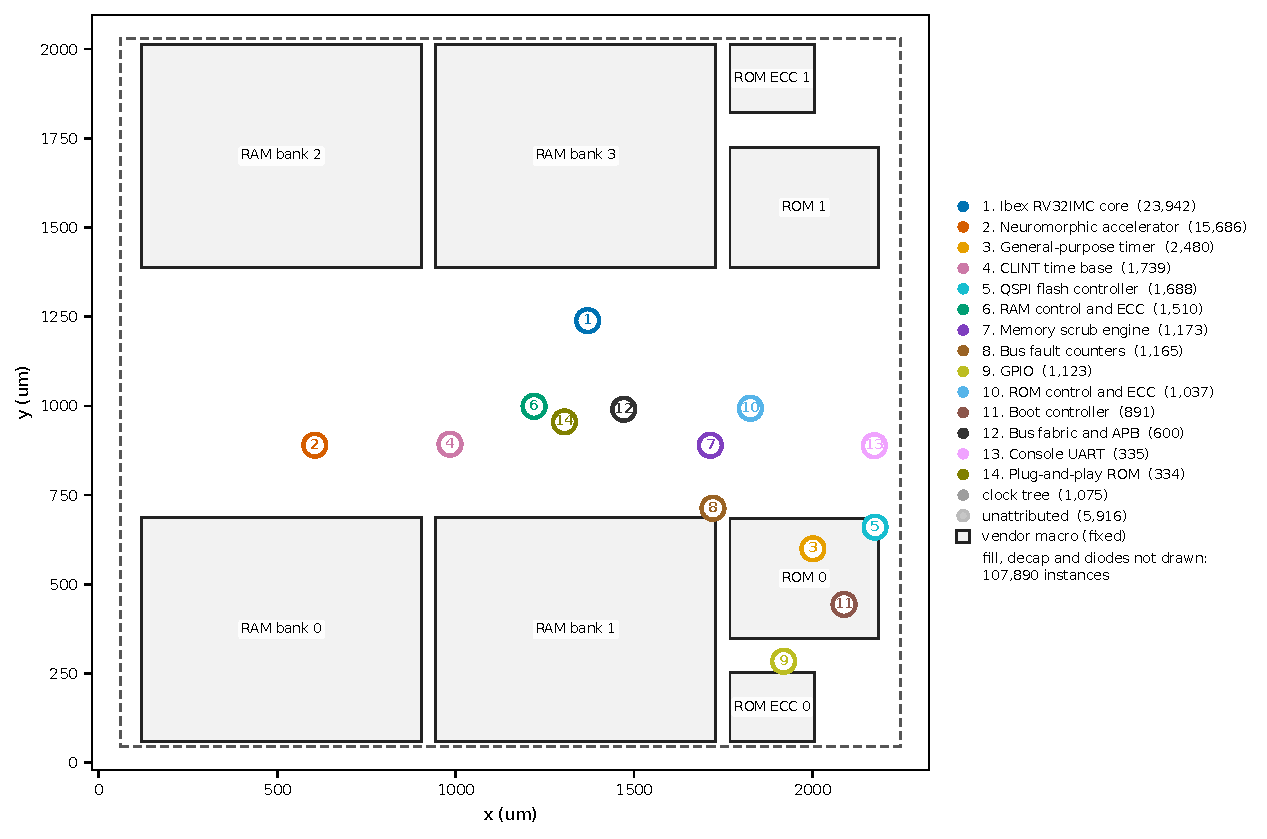
\includegraphics[width=\linewidth]{figures/layout_blocks.pdf}
  \caption[The system-on-chip, as placed]{The whole die, with every
  standard cell coloured by the block it belongs to and the eight vendor
  memory macros drawn and labelled, read out of run
  \code{s83romecc5}'s own DEF and netlist --- the eight-macro layout of
  \dcite{67}{section 11}. The die is
  2306.40 by 2075.22\,\si{\micro\metre}, that is
  \qty{4786287.408}{\micro\metre\squared} (\dcite{59}{section 3.1}). Apart
  from the eight macros, which are fixed, nothing here was told where to
  go: the clusters are the placer's, not the designer's. Only about
  7{,}700 of the die's instances still carry a hierarchical name after
  synthesis --- the generator's docstring figure, beside a comment in
  the same file counting 1{,}140 instance names with a dot in them ---
  so the block attribution is made by connectivity --- nets
  keep their hierarchical names, each anonymous cell takes the block
  most of its pins' nets vote for, and two rounds of neighbour
  propagation follow --- and the
  \qty{9.75}{\percent} that never resolves is drawn grey and counted in
  the legend rather than hidden
  (\code{make\_layout\_figures.py} and
  \code{layout\_attribution.json}, both in \code{thesis/figures/}).
  Read the per-block
  counts as an attribution with that error bar on it, not as a census.}
  \label{fig:intro-blocks}
\end{figure}

\Cref{fig:intro-blocks} is the part. It carries 168{,}592 instances, of
which eight are the vendor SRAM macros and 168{,}584 are standard cells;
the two largest attributed blocks are the Ibex core at 23{,}942 cells
and the accelerator at 15{,}686, and 107{,}890 of the total are fill,
decap and diode cells that belong to no block and are not drawn
(\code{thesis/figures/layout\_attribution.json}). Those per-block
figures are the output of the attribution method described in the
caption, and the method's own 9.75\,\% unattributed remainder is the
error bar that travels with every one of them. A reader who wants a
census of a block should take it from that block's synthesis record, not
from this picture; what the picture is for is the question
``where is the processor, where is the memory'', which no table answers
as quickly.

\section{What this is not}
\label{sec:intro-not}

Four negatives bound everything that follows, and each is a matter of
record rather than of modesty.

\textbf{There is no silicon of this system-on-chip, and no tape-out of
it.} Nothing in the repository has been fabricated
(\dcite{00-index}{section 2.2}). The one design that has been submitted
anywhere is the pilot of \Cref{sec:intro-two-parts}, and even there the
shuttle slot was still an open owner action at the time of writing, with
the close at 2026-09-21 20:00 UTC (\code{ROADMAP.md} section 4 item 1).
A full-SoC run is gated on two things the pilot cannot settle: the SRAM
macro sign-off blocker of \Cref{sec:intro-pdk}, which is upstream, and a
timing constraint the layout does not meet (\code{ROADMAP.md} section 1).

\textbf{No clock frequency is claimed for this design.} This is a rule,
not an omission, and \Cref{sec:intro-rules} gives its three reasons. The
consequence for the reader is that every timing result in this document
is reported as a period, a slack and a corner name, in the words the
tool used: the system-on-chip is constrained at a 20\,ns period and
misses it by \qty{-3.2029}{\nano\second} on 2{,}003 endpoints at the
\code{nom\_slow\_1p08V\_125C} corner under a real 5\,\% derate
(\dcite{47}{section 8.2}), and on the layout that also contains the
accelerator by \qty{-3.5789}{\nano\second} on 2{,}175 endpoints
(\dcite{61}{section 8.1}). Those two numbers differ by
\qty{0.3760}{\nano\second}, which is inside the roughly
\qty{0.4}{\nano\second} of instrument resolution \dcite{44}{section 5.2}
measured, so that difference is not reported as a regression in either
direction (\dcite{61}{section 8.1}). Neither of them is the current
layout's figure, and this document does not let them stand in for it:
on the eight-macro run of \Cref{sec:intro-pdk} the same corner reads
\qty{-7.5758}{\nano\second} on 3{,}529 endpoints, and
\qty{-7.3492}{\nano\second} on 3{,}550 after the antenna repair
(\dcite{67}{section 11}).

\textbf{There is no radiation test data.} No total-dose, proton or
heavy-ion result exists for anything built here; the fault-injection
campaigns are simulations of single-bit upsets, and the documents that
report them say so in their own limitations sections
(\dcite{00-index}{section 2.2}). Every reliability statement in this
work is therefore pre-silicon.

\textbf{There is no flight heritage, and the reference has it.} The
positioning documents are explicit that the incumbent's advantage is
institutional: Gaisler's GR712RC and GR740 fly \textbf{[fact]}, which
makes the GR801 the default choice for a mission that must show
qualification paperwork to an agency customer --- an inference that
document tags \textbf{[estimate]} rather than a measured share
(\dcite{05}{section 1.1}). This project does not
compete with that and the positioning rules forbid implying that it
does: the device is described as fault-tolerant by architecture on a
commercial bulk 130\,nm process, never as radiation-hardened, with a
stated LEO class of 10--30\,krad(Si) pending test data
(\dcite{05}{section 4}, rules 1 and 2).

\begin{sloppypar}
One further caution belongs here because it is the sharpest disagreement
inside the corpus. \dcite{00-index}{section 1} describes the work as
``a clean-room retarget, not a clone''. \dcite{14}{section 11.2} records
that the decision that would license that phrase --- \code{docs/02}'s open
question 2, whether Solderpad-licensed reference RTL was reused, used
only as a golden model, or not at all --- is \emph{still open}, and
states the consequence plainly: until it is answered, no public
description of this accelerator may claim independent implementation.
\dcite{78}{section 5} repeats it as a live item on the published mirror.
This document therefore does not make that claim. It describes what the
accelerator does, what it was verified against, and where its
architecture came from, and leaves the provenance question where its
owner left it: open, with a date on it.
\end{sloppypar}

\section{The mission case}
\label{sec:intro-mission}

The argument for building this part at all rests on a gap in the market
survey and on a workload sizing that was done late and changed the
project's priorities when it arrived.

The gap first. Across three tiers of space edge-AI silicon --- qualified
rad-hard SoCs, radiation-characterised COTS systems, and flight
experiments with commercial neuromorphic parts --- \dcite{05}{section
2.3} finds no open-architecture device in any tier: no vendor publishes
RTL, verification suites or fault-injection data, so a mission
integrator cannot independently audit anyone's fault-tolerance claims.
It also finds no chip-level neuromorphic product below the rad-hard
tier, between a qualified SoC in the tens of thousands of euro
(\textbf{[estimate]}, \dcite{05}{section 1.2}) and an unrated commercial
part on a custom board. Both findings are recorded as facts by absence
in that survey, the second explicitly kept under review, which is the
correct strength for them. The demand side is not speculative: NASA flew Intel's Loihi on the
TechEdSat-13 3U CubeSat, and BrainChip's AKD1000 has flown in low Earth
orbit on Optimus-1 (\code{docs/05} sections 2.1 and 2.3).

The workload sizing is \code{docs/53}, and it found the project had been
asking the wrong question. \dcite{05}{section 3.4} lists four candidate
mission profiles, all tagged \textbf{[estimate]}, and the only numeral
anywhere in those four bullets is a power figure: orbit-average power in
the tens of milliwatts (\dcite{53}{section 3}). Sized against a flown
instrument --- Falcon Neuro's two event cameras on the International
Space Station, whose paper reports 16{,}700 events/s time-weighted and
53{,}444 events/s recording-weighted with a standard deviation of
134{,}982 --- the heaviest profile costs 10.23\,\% of the cycle budget
at two standard deviations above the mean, the lightest costs 0.0044\,\%,
and the latency profile is met by a factor of 76{,}551
(\code{docs/53} sections 3.1, 6.1--6.4; every one of those percentages is
an \textbf{[estimate]} derived from measured event rates and measured
per-event costs). That document tabulates each profile at two candidate
periods and the figures quoted here are the conservative column of the
two; neither period is repeated in this work, for the reason
\Cref{sec:intro-rules} gives. The same document measured where the cycles actually
go: the serial transport between the processor and the accelerator is
93--98\,\% of every workload measured, an architectural factor of 27
against a clock factor of 1.16 (\code{docs/53} sections 4.2 and 5).

So the binding requirement is power, not throughput, and the power
numbers have themselves been corrected twice. The system-on-chip's
sign-off run carried a \code{report\_power} result with no switching
activity annotated at all --- 27.774, 34.835 and
\qty{46.095}{\milli\watt} at the slow, typical and fast corners
(\dcite{53}{section 7.1}) --- which five documents had described as
``no power number'' while the file sat in the run directory they were
reporting from (\dcite{64}{section 3.4}). Annotated with the measured toggle rates of
the one program in this repository that has a duty cycle in it ---
\code{docs/46}'s time-triggered supervisor, which idles in WFI between
frames, and not the whole-SoC self-test, which is awake for 99.94\,\% of
its cycles --- the same layout gives \qty{33.890}{\milli\watt}
busy and \qty{5.539}{\milli\watt} idle with the core's clock gated in
WFI, and an orbit average of \qty{5.540}{\milli\watt} at the 0.0044\,\%
duty cycle profile 1 was sized at (\code{docs/57} sections 5.1, 5.2 and
11.1). The self-test is the cross-check rather than the source: its
120-cycle post-WFI tail measures \qty{5.619}{\milli\watt}, 1.4\,\% from
a supervisor window three hundred times longer
(\dcite{57}{section 5.2}). That layout does not contain the accelerator
(\dcite{57}{section 3.2}); on layouts that do, the idle figure is
\qty{8.287}{\milli\watt} with an orbit average of
\qty{8.289}{\milli\watt} (\dcite{76}{section 8}), and on the layout
after that, \qty{8.315}{\milli\watt} idle and \qty{22.142}{\milli\watt}
computing --- with no busy figure published as a property of the design,
because that document measures the busy total as a placement's property
and not a design's (\dcite{77}{section 9.5}). Every one of those
numbers is a pre-silicon flow estimate on a layout that fails setup at
the slow corner and fails maximum slew and maximum capacitance, and
\dcite{05}{section 4} rule 5 requires that all of that travel with the
number or none of it does.

The requirement the design does \emph{not} meet is the fourth profile:
long idle mission phases, where an activity-proportional part should
idle at microwatts. \dcite{53}{section 7.3} put the gap at four orders
of magnitude and said nothing in the design was aimed at it. Both halves
of that are superseded, by \code{docs/57}, which landed 2026-09-04 and
whose section 12 items 2 and 4 name them: measured under a duty cycle
the part idles at 4.5 to \qty{7.1}{\milli\watt} across the three corners
rather than 27.8 to 46.1, which puts the gap at about 2.4 orders of
magnitude from ``tens of microwatts'' and about 1.7 from ``hundreds''
(\textbf{[estimate]} for the orders, \textbf{[fact]} for the measured
column), and there is a mechanism, it works, and it covers
\qty{80}{\percent} of the flip-flops (\dcite{57}{section 11.2}). The
requirement is still not met, and it is worth saying here in the
introduction because it is still the largest single unmet requirement in
the record.

\section{Why 130\,nm, and why this PDK}
\label{sec:intro-pdk}

Two questions, and the answers are different in kind: the node follows
from arithmetic, and the particular kit follows from a radiation story
and a memory story.

The arithmetic is \dcite{01}{section 3}. The reference carries 11.2\,MB
of on-chip SRAM. The bitcell ratio between 28\,nm and 130\,nm is about
20$\times$, but open-PDK memory compilers do not reach foundry
array efficiency, so the effective memory-density gap between the
reference's platform and an open 130\,nm flow is 70--90$\times$
(\textbf{[estimate]}, \dcite{01}{section 3.2}). Memory, not logic, sets
the scaling factor: a 25\,mm\textsuperscript{2}-class die supports
roughly 100--128\,KB of SRAM, a 64--128 MAC
event-driven fabric, an RV32 management core and the low-speed interface
set (\textbf{[estimate]}, \dcite{01}{section 3.4}). That figure has to
travel with its PDK, because the document forbids quoting it otherwise:
every 130\,nm density in \code{docs/01} section 3 is SKY130-derived, and
on the SG13G2 kit actually selected the same section's comparison puts
the budget at 256--512\,KiB, two to four times as much
(\textbf{[estimate]}, an assumed band pending \code{docs/04} open
question 2). A 1:1 retarget is absurd; a proportional
one is not, because the architecture's multi-pass execution is exactly
the mechanism that lets a small fabric run networks sized for a larger
one (\dcite{01}{section 2.2}).

The node is also where the cost argument lives. Standard-rate access to
the selected process through Europractice is
EUR~7{,}300/mm\textsuperscript{2} with a 10\,mm\textsuperscript{2}
minimum, so a minimum-size run is EUR~62k--73k and out of scope; the
open-source MPW rate of
EUR~1{,}000--2{,}800/mm\textsuperscript{2} puts a
12\,mm\textsuperscript{2} MVP die at EUR~12k--34k, which brackets the
comparable SKY130 commercial shuttle at \$14{,}950, and the whole MVP
envelope including packaging, boards and an optional total-dose campaign
lands at roughly EUR~20k--65k (\code{docs/04} sections 5.1 and 5.3;
the band on the realised open-source price is the single biggest cost
unknown and that document says so).

The particular kit is IHP SG13G2, with SkyWater SKY130 as the fallback,
and \dcite{04}{section 2} gives five reasons in order. The first is that
\emph{the radiation story is the product}. IHP has published
characterisation of its 130\,nm family through an ESA paper covering the
rad-hard sibling PDKs, and that data is a genuine asset --- but the same
section carries a correction dated 2026-08-29 that is more instructive
than the data: an earlier revision had recommended putting a specific
heavy-ion number into the project's own claim sentence, and it was taken
out, because the figure measures sibling-PDK standard-cell test
vehicles and a reader of that sentence would reasonably take it as a
property of the part being described. The published numbers stay in the
sourced-facts list where their attribution travels with them, and the
claim sentence says only ``130\,nm family with published ESCC-track TID
and SEL characterization'' plus this project's architectural hardening.
Nothing in the repository measures the single-event latch-up behaviour
of anything this project has built. The second reason is the European
institutional ecosystem; the third is that the open PDK~\cite{ihppdk}
ships foundry compiled SRAM macros with a built-in BIST interface
rather than compiler-generated cells (\code{docs/04} section 3); the
fourth is the cost argument of the paragraph above; and the fifth is that the fallback
is unusually strong, because the flow is already silicon-proven on the
fallback node~\cite{openlane2020}, so falling back costs a retarget
rather than a flow rebuild (\textbf{[estimate]} at 3--6 weeks, \dcite{04}{section 2}).

\begin{figure}[tbp]
  \centering
  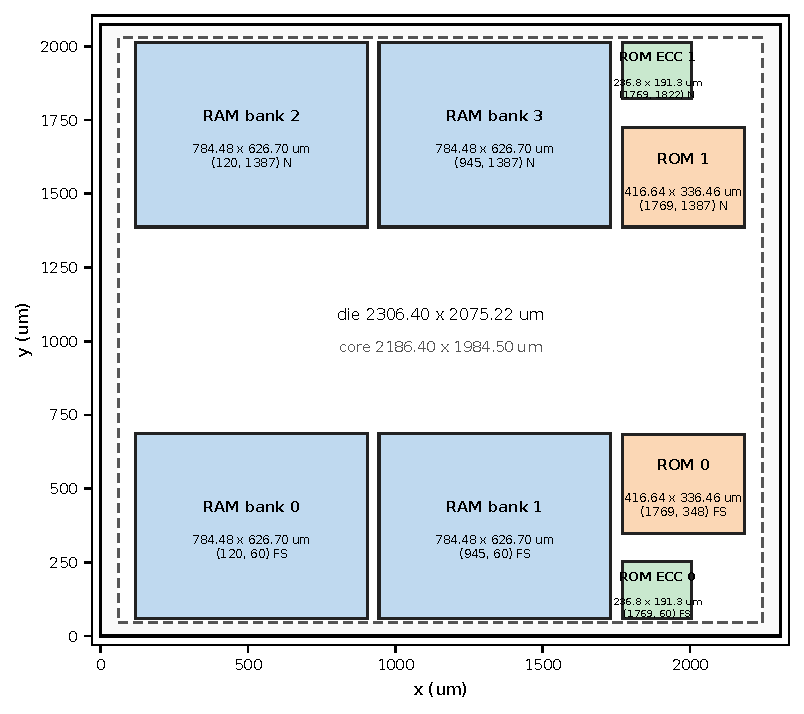
\includegraphics[width=\linewidth]{figures/floorplan_macros.pdf}
  \caption[Floorplan and the eight vendor macros]{The die outline, the
  core area and the eight vendor SRAM macros with their names, sizes and
  coordinates, drawn from the sign-off run's own DEF
  (\code{thesis/figures/make\_layout\_figures.py}). Four
  \code{RM\_IHPSG13\_1P\_2048x64} macros carry the RAM, two
  \code{1024x32} macros the boot ROM and two \code{512x16} macros the
  ROM's check bits. These are the parts the open decks cannot sign off
  (\dcite{12}{section 8}), which is why every geometric result in this
  work is reported as inside the macro hierarchy or outside it rather
  than as a total.}
  \label{fig:intro-macros}
\end{figure}

The third reason is also where the project's largest external blocker
lives, and \Cref{fig:intro-macros} is the picture of it. The macros the
open PDK ships cannot be signed off by the open decks at the pinned PDK
version. A trial harden containing one of them completed every flow
stage and ended with 1{,}106{,}478 Magic DRC error boxes, 2{,}316
KLayout DRC errors and 359 Netgen LVS errors --- and every one of the
Magic boxes, and every KLayout item, was \emph{inside the macro's own
footprint}, with the standard-cell area, the power grid and the routing
clean (\dcite{12}{section 7.5}). That Magic figure is a count of error
boxes and not of distinct violations: the flow's own report prints
``Should be divided by 3 or 4'' beneath the total, which puts the
distinct count at roughly 277{,}000--369{,}000 (\textbf{[estimate]}, the
report gives a range and not a divisor), and \dcite{12}{section 7.5}
quotes the raw box count everywhere with that caveat attached. The
conclusion does not depend on which end of the range is right: the
smallest reading is still hundreds of thousands of violations against a
required zero, and \dcite{12}{section 8} recorded a NO-GO for this PDK
version thirteen days before the gate that asked for it (\code{ROADMAP.md}
section 1). Two of the LVS
causes were diagnosed in that document --- hierarchy names that disagree
between the CDL and the extracted layout, so Netgen flattens the macro,
and bus index delimiters that disagree between angle brackets and square
brackets, so none of the macro's 188 bus pins match --- and the LVS half
is an open upstream issue.

That is why the geometric results on the eight-macro layout are stated
the way they are. On the \code{s83romecc5} layout, Netgen reports
\code{Circuits match uniquely} with all seven LVS counters at zero
(deck run \code{s83lvsbb2}), read
for exactly what it is: the vendor macro is a black box on both sides,
so the match signs off the connectivity \emph{into} the macros' pins and
says nothing about their internals. The KLayout deck declares 173 rule
categories in 47 groups and three fire, for 11{,}048 markers over 204
distinct cells --- 6{,}584 distinct shapes, because two of the three
rules are evaluated over the same derived layer and report an identical
set --- of which zero are outside the vendor macro hierarchy. The
abstracted Magic run reports 170 error boxes on \code{s83romecc5},
20 inside a macro
footprint and 150 outside, and every one of the 150 lies within
\qty{0.500}{\micro\metre} of a macro edge, none in open routing area,
because a LEF obstruction blanket is one shape more than
\qty{10}{\micro\metre} wide and ordinary routing beside it violates
wide-metal spacing rules that the macro's real geometry would not
(\dcite{67}{section 11}). \code{README.md} summarises the run with 182
Magic boxes and 162 outside, which reads like a contradiction and is
not one: 182 and 162 are run \code{s83ant}, the same layout with its
two antenna violations repaired, and the 60 diodes that repair inserted
moved routing inside the same halo --- 20 inside a footprint in both,
all 162 still within the same half micron, and the KLayout figures
identical marker for marker (\dcite{67}{section 11}). That is the shape
\Cref{sec:intro-rules} is about, and it had to be applied to this
chapter's own reading of its sources before it could be written down:
two correct statements about two different inputs, quoted without
saying which.

\section{Two parts: a frozen pilot and a system around it}
\label{sec:intro-two-parts}

The work is deliberately split in two, and the strategy is stated in
\code{ROADMAP.md} section 1: silicon-prove the PDK, the flow, a slice of
the inference fabric and the hardening demonstrators on a cheap shuttle
run before committing a full SoC.

\textbf{The pilot} is \code{tt\_um\_melihakbulut\_nssoc}, a
$6\times2$ = 12-tile design on the TTIHP26b shuttle, die area
\code{0 0 1289.28 313.74}\,\si{\micro\metre}, frozen at commit
\code{b6738e5} (\dcite{34}{section 1}). Its sign-off run closes setup at
every corner --- the slow corner at \qty{+1.2262}{\nano\second}, quoted
here to four decimals from a metric that carries more digits
(\code{+1.226180081066267}) --- with hold at
\qty{+0.1029}{\nano\second}, 33{,}564 instances at 48.7516\,\%
utilisation, and zeros for Magic DRC, LVS, detailed-route DRC, antenna
nets and pins, and total negative slack at all three corners, under a
5\,\% derate written into the flow's own constraint file
(\dcite{34}{section 3.3}). The Tiny Tapeout precheck passes 10 of 10
(\dcite{34}{section 7}). Its measured upset behaviour is a campaign of
378 injections classified against the golden model: 97 masked
(25.7\,\%), 193 corrected (51.1\,\%), 82 detected (21.7\,\%), 6 silent
data corruptions (1.6\,\%), 0 hangs, in 445.7\,s
(\dcite{64}{section 3.1}). At gate level, 370 of 370 comparable
injections classify identically to RTL (\dcite{32}{section 5.1}, quoted
by \code{README.md}).

The point of \code{docs/34} is not the numbers but the pinning: it answers
one question --- \emph{is what I am submitting the thing that was
verified?} --- and answers it so the answer can be checked by running
commands~\cite{lamb2022}. Ten RTL blobs by git hash, the submission tree
by a 31-file manifest whose own SHA-256 is recorded, six flow configurations pinned
by hash inside their own generator, and the built netlist, powered
netlist and DEF bit-identical across four independently configured
hardens of two configurations on two dates
(\code{docs/34} sections 2.1, 3.1, 3.2, 4 and 5.1). The GDS files differ
between those runs and that is expected, because GDS carries an embedded
generation timestamp: the GDS hash is a provenance record and not an
equality criterion, and the geometric equality is established by the
decks instead (\dcite{34}{section 3.2}).

What remains on the pilot is not engineering. The shuttle closes
2026-09-21 at 20:00 UTC, and the slot costs EUR~955 --- twelve tiles
at EUR~70 is EUR~840, plus a EUR~300 devkit subsidised to
EUR~100 while any of the subsidised boards remain, plus EUR~15 of
shipping (\code{docs/37} section 5 items 1 and 2, with the price table
both were read from in that document's section 1). Both the date and the price are
owner-side facts read from the vendor's own published records on
2026-08-31, and the close carries a time the project's earlier documents
did not record: 20:00 UTC, not local midnight (\dcite{37}{section 1}).
Buying the slot is the one item in \code{ROADMAP.md} section 4 that a
person must still do.

\textbf{The system-on-chip} under \code{hw/soc} is everything else. It
was begun after the pilot froze, it instantiates the frozen pilot rather
than copying it --- \code{hw/rtl/pilot\_top.v} inside \code{soc\_top.v},
reached over the same four serial pins the die will have --- and a
program running on Ibex out of the boot ROM configures it, loads its
weights, feeds it a six-frame event stream and reads the spikes back
against an answer the golden model computed at build time: 27 checks,
fail mask 0 (\code{docs/51}). The transport is serial because that is what
the die has, which costs 176 clock cycles per register access
(\dcite{53}{section 4.1}) and buys exactly one implementation of the
die's host protocol, the one in the system's own regression.

The freeze rule is what keeps the two apart. \dcite{34}{section 9}
states what does and does not void it: documents, tests and analysis
over existing run trees do not; any non-comment change to
\code{hw/rtl}, to the submission sources or to a pinned configuration
forces a full re-harden and a gate-level re-run. That rule has been
exercised twice --- once when two checkers were bound to all corners,
which forced a re-harden that reproduced the superseded runs on 196 of
196 and 194 of 194 metrics with the netlist bit-identical, and once when
the licensing decision added SPDX headers to every file in
\code{hw/rtl}, where all ten blobs moved and the netlist did not
(\code{docs/34} sections 1, 2.1 and 3.3). Both times the record was amended in
place with every superseded hash retained, because a freeze record that
can only be checked against \emph{now} is not a freeze record.

\section{Where the work is published}
\label{sec:intro-publication}

\begin{sloppypar}
The development repository is private and the published tree is a
generated mirror of it. \dcite{78}{section 1} takes that decision and
records what it costs: \code{scripts/gen\_public\_mirror.py} writes the
published subset into a directory and makes one commit naming the source
revision, it does not push and it does not create a repository, so
publication stays an act of the owner. The alternative --- making the
development repository public --- was declined for one honest reason:
three hundred-odd commit messages written over three weeks have not been
audited, and one missed message is not recoverable after a push
(\dcite{78}{section 1.1}). The mirror's cost is stated in its own
\code{README.md} rather than left for a reader to notice: you cannot see
how the design got here from the published repository, only where it
arrived. What makes that cost bearable is the corpus, which records the
withdrawn claims and the re-attributed measurements that a commit log
would not hold --- the history is published, it is just not in
\code{git log}.
\end{sloppypar}

\begin{sloppypar}
Three licences apply, one per kind of thing, decided in \code{docs/14} and
signed on 2026-09-09 (\dcite{14}{section 11}): CERN-OHL-W-2.0 for RTL,
testbenches, constraints, formal jobs and flow configuration;
Apache-2.0 for generators, golden models, harnesses, flow drivers,
analysis and CI; CC-BY-4.0 for the documents in \code{docs/} and the
measurement data. The reasoning is in \code{docs/14} sections 6.1--6.3 and
the load-bearing part of it is that the outbound choice was
\emph{unconstrained}: every inbound licence that touches a tracked file
is permissive, because third-party trees are fetched into gitignored
directories rather than vendored, so inbound obligations attach in only
two tracked places --- the Apache-2.0 Tiny Tapeout template scaffolding
under \code{tt/}, and two corrected copies of riscv-formal's own
instruction models, which carry upstream's ISC notice inline
(\code{docs/14} sections 2.1, 2.2 and 5.0). The reciprocal licence for
hardware was chosen against the permissive one for a stated reason:
the project's claimed differentiator is auditability, and a licence that
lets a derivative be closed undercuts the claim
(\dcite{14}{section 6.1}).
\end{sloppypar}

Three things are held back from the mirror, all commercial and none of
them technical: one section of the positioning document, the funding and
shuttle document, and the drafted text of an unsubmitted application.
Nothing technical is held --- no negative result, no withdrawn claim, no
measurement, no failing check --- and \dcite{78}{section 2} states why
that is a condition rather than a courtesy: a record that publishes only
what worked is a brochure. Each held file is replaced by a stub that
keeps the filename and says what was held, so that the corpus's own
cross-reference test still passes in the generated tree, which it does:
90 of 90 when that section was written (\dcite{78}{section 2.1}), and 95
by the time \dcite{78}{section 7} re-ran it a day later, because it is a
count of documents and not of findings. The mirror was first published on
2026-09-10 at 518 files from source revision \code{93757c9}, and
republished on 2026-09-11 at 529 files from \code{26f4494}
(\code{docs/78} sections 5 and 7).

\section{The rules this work holds itself to}
\label{sec:intro-rules}

A reader who takes nothing else from this chapter should take these
four. Each exists because the project broke it once and wrote down what
that cost.

\textbf{A superseded measurement is reported as superseded, with its
date, and is not rewritten.} This is \dcite{64}{section 2}'s method: the
original sentence stays where it was, struck through where a short
phrase is wrong or left whole and followed by a dated note, and the note
says what the value is now, why the old one was written, and which file
settles it. The document that established it was reconciling seven
figures the corpus stated two ways, and its first verdict is the reason
the rule is worth keeping: \emph{none} of the seven was a transcription
error. Every disagreement was two correct statements about two different
inputs --- an earlier run, a different source list, a different content
--- quoted without saying so (\dcite{64}{section 1}). The pilot's
fault-injection campaign is the clearest case: 335, 366 and 378 are all
real logs of the same file at three commits, and the history of that one
file settles which is the campaign of record without making the other
two wrong (\dcite{64}{section 3.1}). Where this document reports a
figure that a later measurement has moved, it reports both and says
which is which; where two documents in the repository still disagree, as
with the Magic box count in \Cref{sec:intro-pdk}, it says so and cites
both.

\textbf{No clock frequency is published for this design.}
\dcite{53}{section 9.2} refuses it in three ranked reasons. The first is
that the only available number is the frequency a layout happened to
reach, and a requirement written in the units of the answer is not a
requirement --- the derived requirement in that document is not a
frequency at all, it is a count of serial frames per second, and at the
geometry that exists the fabric caps that count long before the clock
does (\dcite{53}{section 6.5}). The second is \dcite{05}{section 4}
rule 5: any figure published externally must be traceable to measurement
or clearly labelled a design target, and the available figure is
neither, because it is the derived maximum frequency of a run that fails
setup on 2{,}003 endpoints, fails maximum slew at the slow corner and
fails maximum capacitance at all three. Half of that second reason has
since been superseded and the half that governs has not: the same
sentence in \dcite{53}{section 9.2} also said the layout had never seen
Magic DRC, KLayout DRC or Netgen LVS, and all four deck families have
run on \code{soc\_top}'s own geometry since 2026-09-11
(\code{README.md}, citing \code{docs/77} and \code{docs/79}); the slew
and capacitance failures are unchanged, and they are the half the rule
now rests on. The third reason is that two parts in
one project would carry two clocks and one of them is being fabricated,
and a reader offered both would ask which one the project's clock is.
What may be said instead is the stronger claim anyway: the mission
profiles have been sized, three of four are met with two to five orders
of magnitude of margin, and the fourth is a power requirement the design
does not meet with the mechanism named (\dcite{53}{section 9.4}).

\textbf{\textsc{timeout}, \textsc{killed} and \textsc{error} are three
different words.} \dcite{63}{section 16} spends thirty lines on the
distinction after a formal job was reported as a timeout and its own log
said otherwise: the job had been sent a signal from outside the run at
1\,h\,41\,m and the tool recorded \code{DONE (ERROR, rc=16)}, while no
timeout had been configured for it to reach. The reading each word
licenses is different. \textsc{timeout} means a bound was set, the job
reached it, and the measurement is complete --- \emph{this engine did
not close in that much time} --- and the jobs entitled to that word
wrote \code{rc=124} into their wall-time files, which is the
\code{timeout} utility saying it sent the signal itself. An error from
an outside kill means no bound was set and no measurement was completed,
and calling it a timeout would silently promote an interrupted run into
a finished experiment. The corpus has made that mistake in both
directions, and the fix is the same either way: read the runner's return
code before choosing the noun. The general form --- ``nothing came''
and ``I arrived late'' are not the same result --- is applied to a
testbench monitor in \dcite{81}{section 4.1}, which attributes the rule
to \code{docs/64} where the passage itself is in \code{docs/63}; both are
cited here because they disagree about the citation and not about the
rule.

\begin{sloppypar}
\textbf{A check must test the property, not the name.} The sharpest
statement of this is \dcite{78}{section 3}, and it is sharp because both
of its instances were in the project's own instruments rather than in
the design. The licence checker searched the first 4{,}000 characters of
a file for an identifier string in any context, so it read its own
docstring as its own licence header and reported zero missing while
carrying no header at all; it now counts a tag only on a comment line in
the first twelve lines, which is where a header is and where prose about
headers is not. The mirror generator carried a guard meant to refuse to
run if a workflow file no longer contained a sentence it rewrites ---
written as ``if the file is in the set'', so when the file was
\emph{deleted} the guard did not fire, it was skipped, and the generator
wrote 511 files as though nothing were owed. \dcite{78}{section 3.2}
records the conclusion in one line: a check that cannot fail when the
thing it checks is absent is not a check. That was the third instance of
the shape in this repository's own instruments and the first found in a
guard written to prevent it. The question is never ``did the check
pass'', it is ``what could the check have seen''. The corresponding rule
when a check is found to be narrow is \dcite{50}{section 8.1}'s:
\emph{extend, do not relax}.
\end{sloppypar}

Underneath all four sits a labelling convention used in every document
and carried into this one. \textbf{[fact]} means measured in this
environment or read out of a file; \textbf{[estimate]} means derived or
judged; \textbf{[planned]} means an intention with a date attached and
nothing behind it yet (\code{docs/00-index}, and the same three words at
the head of most documents in the corpus). Where a source marks a
statement with one of these, this document carries the mark rather than
flattening it.

\section{What this document is}
\label{sec:intro-status}

This is a record of measurements taken with open tools on a design that
exists in register-transfer and layout form. It is not a qualification
report and nothing in it should be read as one.

Concretely: there is no beam test, no lot, no screening and no
qualification body~\cite{ecss60_15c}; the fault-injection results are
simulated single-bit upsets, not measured event rates~\cite{nijsink2026};
the timing, power and area figures are pre-silicon flow results on layouts that are explicitly named where they
fail; and the memory macros the design depends on cannot be signed off
by the open decks at the pinned PDK version, so the die that carries
them cannot be either (\dcite{67}{section 11}). The claims this work
does make are of a different kind --- that a given mechanism is present
in the shipped netlist rather than only in the source, that a given
property holds over all reachable states, that a given campaign
classified a given number of injections a given way, that a given deck
found a given number of markers in a given place --- and each of them is
quoted here against the document that measured it, which in turn names
the command and the run tree it was read from.

\section{Road map}
\label{sec:intro-roadmap}

The remaining chapters are organised by what they measure rather than by
the order in which the work happened.

\textbf{The architecture chapter} describes the system as built: the
bus, the memory map frozen as a single generated source, the interrupt
and timing subsystem, the watchdog and its escalation ladder, the
peripherals, and the boot flow that initialises every word of an
error-correcting RAM before anything reads it --- because a memory whose
rows carry check bits powers up with an uncorrectable word everywhere,
not a zero. Its sources are \code{docs/38} through \code{docs/41},
\code{docs/65}, \code{docs/66} and \code{docs/68}.

\textbf{The accelerator chapter} describes the event-driven inference
engine, the register map generated from a single source, the serial
transport to it and what that transport costs, drawing on \code{docs/02},
\code{docs/10}, \code{docs/51} and \code{docs/53}.

\textbf{The hardening chapter} prices every protection mechanism
separately, because the project's discipline is that nothing is
protected before it is measured and every protection reports what it
cost: triple-modular redundancy on the state that cannot recover, SECDED
on the memories and the architectural register file, a scrub engine, and
fault counters an operator can read. Its sources are \code{docs/43},
\code{docs/44}, \code{docs/55}--\code{docs/58}, \code{docs/67} and \code{docs/69}.

\textbf{The verification chapter} covers the five layers and what each
can and cannot see: the cocotb regressions, the \emph{guards} that read
the tree without simulating it, the SymbiYosys property sets, the
riscv-formal bring-up against the ISA, and the seeded fault-injection
campaigns at register-transfer and gate level --- every one of them
judged against the bit-exact golden models that are the specification
(\code{docs/09}, \code{docs/11}, \code{docs/16}, \code{docs/32}, \code{docs/42},
\code{docs/52}, \code{docs/63}, \code{docs/74}, \code{docs/82}).

\textbf{The physical chapter} takes the design through the flow: the
floorplan and the decision behind it, the macro placement, synthesis,
place and route, the geometric decks and their macro-scoped results, and
the reproducibility record (\code{docs/12}, \code{docs/45}, \code{docs/47},
\code{docs/48}, \code{docs/59}, \code{docs/61}, \code{docs/71}, \code{docs/77},
\code{docs/79}). The layout figures introduced here are read in detail
there.

\textbf{The results chapter} puts the measurements side by side: what
closes, what does not, what each mechanism cost in area and in slack,
and what the power figures say once real switching activity is annotated
(\code{docs/57}, \code{docs/60}, \code{docs/76}, \code{docs/77}).

\textbf{The concluding chapter} states what remains open, in the terms
the record uses: the upstream macro blocker, the unmet idle-power
requirement, the serial transport that \dcite{53}{section 9.3} ranks
above timing, the provenance question of \Cref{sec:intro-not}, and the
one measurement nothing here substitutes for, which is silicon.

% SPDX-FileCopyrightText: 2026 Hasan Melih Akbulut
% SPDX-License-Identifier: CC-BY-4.0
%
% Chapter 2: the architecture of the system-on-chip. Every number in
% this file is cited to a document or a source file in this repository.

\chapter{Architecture}
\label{ch:arch}

The part is \code{soc\_top}: a 32-bit RISC-V management core, a system
fabric, a memory subsystem with a code over every stored bit, a
core-local interruptor, a general-purpose timer carrying a three-stage
watchdog, a boot controller, two telemetry blocks, a console UART, a
GPIO port, a QSPI flash controller, two plug-and-play device tables and a
spiking-neural-network node built around a frozen shuttle die
(\dcite{60}{}, revision 0.2, 14 September 2026). Its datasheet gives its
status in three words: preliminary, pre-silicon, pre-sign-off.

One sentence travels with the rest of this chapter. \textbf{This design
publishes no clock frequency}, by a rule adopted in
\dcite{53}{section 9.2} and restated in \dcite{60}{section 0}: the
20\,ns period below is the constraint the synthesis and place-and-route
flows were run against, and every slack here is measured against it. It
is not converted into a rating and no rating is implied.

There is no block diagram in this chapter: \cref{fig:arch-panels} shows
where the placer actually put each block, and the floorplan and the
density map belong to the physical-design chapter.

\begin{figure}[tbp]
  
\includegraphics[width=\linewidth]{figures/layout_panels.pdf}
  \caption{Where each block landed. Nine small multiples, one per block,
  each drawing that block's standard cells against a grey die with the
  eight vendor memory macros outlined. Hierarchy barely survives this
  flow's synthesis: of the 168,592 instances in the sign-off run's DEF
  --- 168,584 standard cells and the eight macros --- only 1{,}140 still
  spell a dot in their name, 632 of them the RAM's, and by the script's
  own prefix test exactly one carries a top-level block name. The rest
  are attributed by connectivity --- nets keep
  their hierarchical names, each anonymous cell takes the block most of
  its nets vote for, and two rounds of neighbour propagation follow
  (\code{thesis/figures/make\_layout\_figures.py}). The method leaves a
  remainder: \textbf{5{,}916 of the 60{,}694 logic cells, 9.75\,\%, are
  unattributed} and are drawn grey rather than hidden
  (\code{thesis/figures/layout\_attribution.json}). Nothing here was placement-constrained except the macros, so the
clusters are the placer's.}
  \label{fig:arch-panels}
\end{figure}

\section{The management core}

\begin{sloppypar}
The core is lowRISC Ibex in the \code{small-pmp} configuration: RV32IMC
with physical memory protection at four regions, a two-stage pipeline, a
flip-flop register file, no instruction cache, no branch-target ALU, no
writeback stage, no branch predictor. \code{hw/soc/rtl/soc\_top.v} sets
\code{BaseIsa} = 0 (RV32I), \code{RV32M} = 2 (RV32MFast),
\code{RV32B} = 0, \code{RV32ZC} = 0 (Zca), \code{RegFile} = 0
(flip-flop), \code{PMPEnable} = 1, \code{PMPNumRegions} = 4,
\code{PMPGranularity} = 0, \code{MHPMCounterNum} = 0 and
\code{SecureIbex} = 0.
\end{sloppypar}

\begin{sloppypar}
The core is vendored pristine at commit
\code{34b0705760ef3dfa00e99637432473d2be8f22f3}, Apache-2.0, and
converted to Verilog-2005 by sv2v: 30 of 30 RTL modules and 8 of 8
vendored primitives, 15{,}873 lines, zero errors and \textbf{zero patches
to Ibex} (\dcite{38}{sections 2, 4.2}). \textbf{No equivalence between
the SystemVerilog and the converted Verilog was proven}, because
upstream's own equivalence script drives a proprietary tool this project
does not have. Two corroborations were run instead --- two independent SystemVerilog
front-ends landing within \textbf{0.89\,\% of cell area and two
flip-flops}, and a self-checking program executing in Icarus --- and
\dcite{38}{section 5} refuses to call either a proof.
\end{sloppypar}

\begin{sloppypar}
PMP was not taken for free. \dcite{09}{part B track 3} had already chosen
a software architecture whose isolation mechanism is PMP, so a core
without it does not implement the design already decided. It costs
\textbf{43{,}634\,$\mu$m$^2$, $+18.8$\,\%} and \textbf{1.21\,ns} of
pre-layout closing period, because the address-match logic is replicated
per region and sits in the load/store path
(\dcite{38}{sections 8.4, 8.6}).
\end{sloppypar}

\subsection{Why there is no lockstep}

\code{SecureIbex} is 0: no shadow core, no output comparison, no dummy
instructions, no reset-all flops, no memory-interface ECC. In this Ibex
those are not separable. \code{ibex\_top.sv} lines 212--216 make
\code{Lockstep}, \code{ResetAll}, \code{DummyInstructions} and
\code{RegFileLockstepECC} localparams of \code{SecureIbex}, and
\code{MemECC} defaults to it at line 41 (\dcite{38}{section 3.3}). It is
one switch, and it was priced before it was thrown --- each
configuration synthesised at its own closing period
(\dcite{38}{section 8.4}):

\begin{center}\small
\begin{tabular}{lrrrr}
\toprule
Configuration & Cells & Flip-flops & Area, $\mu$m$^2$ & kGE \\
\midrule
\code{small}, no PMP        & 15{,}736 & 1{,}950 & 232{,}049 & 31.97 \\
\code{small-pmp}, chosen    & 18{,}921 & 2{,}106 & 275{,}683 & 37.99 \\
\code{small-pmp-sec}        & 40{,}236 & 4{,}975 & 585{,}233 & 80.64 \\
\bottomrule
\end{tabular}
\end{center}

Lockstep is \textbf{$+309{,}550\,\mu$m$^2$, $+112$\,\%} over the chosen
core and costs almost nothing in closing period, 0.27\,ns, because the
shadow core is parallel rather than in series (\dcite{38}{sections 8.5,
8.6}).

Area is not what decided it. Lockstep \emph{detects} where this project's voters \emph{mask} (this
Ibex's lockstep is one shadow core and a comparison; a triple core
lock-step votes and therefore masks as well~\cite{tcls2019}); the two
cover disjoint structures, so their costs add rather than share; and the one real overlap, ECC
over the register file, duplicates a codec this project already owns.
\code{MemECC} follows \code{SecureIbex}, so the instruction and data
buses would become 39 bits wide all the way to memory with the check bits
\emph{stored} rather than regenerated: a 22\,\% SRAM overhead on every
byte the CPU touches. \textbf{The owner chose \code{small-pmp} on
2026-08-31} (\dcite{38}{section 10 item 4}), and the same section records
what the choice takes on: the management processor becomes the least
hardened block in the design, its own fault-injection campaign stops
being deferred work, a recovery policy becomes required rather than
optional, and the decision is cheap to reverse only before floorplanning.

\begin{sloppypar}
What has happened since: the campaign was run, the register file gained a
(39,32) SECDED codec with a background scrub at
$+38{,}050.5762\,\mu$m$^2$ and $+222$ flip-flops (\dcite{43}{}), and the
watchdog is the recovery policy. The core as shipped is \textbf{22{,}338 cells, 2{,}328
flip-flops, 316{,}051.6590\,$\mu$m$^2$} (\dcite{45}{section 6.2});
everything in Ibex except the register file remains unprotected, by
decision (\dcite{60}{section 9.8}).
\end{sloppypar}

\section{The bus fabric}

Ibex presents two masters, an instruction port and a data port, each
speaking a simple request/grant/response protocol; it has no AHB, no AXI
and no burst. The interconnect takes that protocol as the internal fabric
and puts \emph{real} AMBA 3 APB at the peripheral boundary.
\textbf{There is no AHB in this SoC and none is claimed}
(\dcite{39}{sections 3, 4, 7}).

The obvious argument, area, is the one the record refuses. An honest AHB-Lite cost probe was built and synthesised at \textbf{17{,}154.32\,$\mu$m$^2$ against
14{,}807.32}, $+15.9$\,\% on the fabric and \textbf{$+0.85$\,\% of the
CPU}. Nine tenths of one per cent is not a reason to reject a bus; what
the measurement is good for is excluding the opposite mistake, that the
decision was made by picking the smaller thing (\dcite{39}{section 6.3}).

Five arguments decided it. \dcite{08}{section 3} defines proximity to
the reference family at the software-visible layer --- addresses,
register maps, slot geometry, discovery tables --- and the wires between
core and RAM are not in it. Not one peripheral core the IP survey
selected is AHB-native, so every one needs a wrapper whichever bus is
chosen, and an APB wrapper is the smaller one. \dcite{08}{row 1}'s
``single AHB-lite layer'' with three masters is a category error, because
\textbf{AHB-Lite has exactly one master by definition} and Ibex alone
supplies two. And AHB folds ``your request was accepted'' and ``your
response is here'' onto one wire, so an arbiter that back-pressures a
master simultaneously tells it its outstanding data phase has not
completed; the probe parks the response instead, and \textbf{67 of the
arbiter's 71 flip-flops are parking registers}.

Evidence settles the rest: nothing in the pinned toolchain is an AHB
protocol checker, while APB's eight-odd rules are proved by k-induction
against ghost registers independent of the bridge's own storage
(\dcite{39}{section 5.3}).

\code{soc\_bus.v} carries two masters onto \textbf{six slave ports} ---
\code{ram}, \code{rom}, \code{clint}, \code{npu}, \code{apb},
\code{pnp} --- plus an internal error slave (\dcite{60}{section 5.2}).
Three of its properties are decisions. It allows \textbf{two outstanding
requests per master}, because Ibex's prefetch buffer issues two and one
would halve instruction-fetch bandwidth. \textbf{All of a master's
outstanding requests must go to one slave}, because Ibex requires
in-order responses and slaves differ in latency; the alternative was a
reorder buffer that must store a whole response, and the restriction
costs one dead cycle when a master changes region. And arbitration is
\textbf{round-robin}, which makes no-starvation a property of this file
rather than an argument about the core: the measured worst gap between
grants is 2 cycles against an asserted bound of 8.

An unmapped access is a \textbf{bus error, never a read of zero}: the
error slave is inside the fabric, always ready, and Ibex turns its
response into an access fault. Properties F1--F9 prove one-hot decode against the generated map
constants, the outstanding limit and that no response is lost or
duplicated. \textbf{Neither formal job proves liveness}: nothing says a
transfer ever completes (\dcite{39}{sections 5.3, 5.5}).

On the one recipe every block here is measured with --- Yosys
\code{stat -liberty} on \code{ihp-sg13g2} typical, \code{abc} at a 20\,ns
target, one gate equivalent $=$ 7.2576\,$\mu$m$^2$ (\dcite{45}{section 6})
--- the fabric is 868
cells, 55 flip-flops, \textbf{10{,}928.8872\,$\mu$m$^2$}, 3.96\,\% of the
unprotected core, and the APB bridge 201 cells, 94 flip-flops,
6{,}437.4912\,$\mu$m$^2$ (\dcite{60}{section 5.2}).

\section{The memory map, and its single source}

\begin{sloppypar}
\code{regmap/memmap.yaml} \emph{is} the memory map. It is not a table in
prose: \code{regmap/generate\_memmap.py} emits the reader's document, the
Python constants the test suites use, the RTL's address decoder, both
device tables' contents, the C header the bare-metal programs include and
the linker's \code{MEMORY} block, and \code{sw/tests/test\_memmap.py}
fails if any is stale (\dcite{39}{section 2.1}).
\end{sloppypar}

\begin{sloppypar}
Three rules are enforced by the generator rather than commented. Ibex resets to \code{\{boot\_addr\_i[31:8], 8'h80\}}, so the generator
derives the reset vector and refuses a boot region that does not contain
it or cannot execute it. Ibex's \code{mtvec} is
256-byte aligned and vectored-only, so \textbf{every region base must be
256-byte aligned} and the map is never itself why a trap vector lands
elsewhere. And every region is a naturally aligned power of two with no
overlaps, so decode is a prefix compare rather than two magnitude
comparisons in the address path of every access.
\end{sloppypar}

\begin{table}[tbp]\small
\setlength{\tabcolsep}{4pt}
\centering
\caption{The system-bus address map, from \code{regmap/memmap.yaml} and
its generated form \code{docs/memmap-soc.md}. Ten regions, six
implemented. Everything outside every region reaches the error slave.}
\label{tab:arch-memmap}
\begin{tabular}{@{}lllllp{5.1cm}@{}}
\toprule
Base & Size & Name & Port & Status & What it is \\
\midrule
\code{0x00000000} & 32\,KiB   & RAM    & \code{ram}   & implemented & System SRAM, SECDED per byte lane, scrubbed \\
\code{0x10000000} & 256\,MiB  & NPU    & \code{npu}   & implemented & Accelerator window; sixteen 4\,KiB node windows \\
\code{0xC0000000} & 8\,KiB    & ROM    & \code{rom}   & implemented & Boot ROM; reset vector at \code{0xC0000080} \\
\code{0xD0000000} & 32\,MiB   & QSPI3  & ---          & reserved    & Flash execute-in-place, 3-byte addresses \\
\code{0xD8000000} & 128\,MiB  & QSPI4  & ---          & reserved    & Flash execute-in-place, 4-byte addresses \\
\code{0xE0000000} & 64\,KiB   & CLINT  & \code{clint} & implemented & \code{msip}, \code{mtimecmp}, \code{mtime} \\
\code{0xF8000000} & 4\,MiB    & PLIC   & ---          & reserved    & Interrupt controller; \cref{sec:arch-irq} \\
\code{0xFE000000} & 16\,MiB   & DEBUG  & ---          & reserved    & RISC-V debug module; there is none \\
\code{0xFF900000} & 1\,MiB    & APB    & \code{apb}   & implemented & Peripheral bridge, sixteen 4\,KiB slots \\
\code{0xFFFFF000} & 4\,KiB    & PNP    & \code{pnp}   & implemented & System-bus device table \\
\bottomrule
\end{tabular}
\end{table}

\begin{sloppypar}
\Cref{tab:arch-memmap} is the map, and every base is taken unchanged from
\dcite{08}{section 3.1}, which took them from the reference family ---
except the NPU window, the one row that document marks
project-specific.  The RAM is \textbf{32\,KiB,
not 64}, since the memory-protection work: the region shrank rather than
the macros growing, and \cref{sec:arch-mem} is why.
\dcite{60}{section 5.3} carries 64\,KiB in its revision-0.1 body with a
dated correction beside it; the map is the normative source.
\end{sloppypar}

\section{The memories}
\label{sec:arch-mem}

There are two implementations of one module name, and which one a reader
is looking at decides what the numbers mean. \code{soc\_mem.v} is
behavioural and is what every simulation and formal job reads;
\code{soc\_mem\_sram.v} is a drop-in with the same module name and port
list built on real vendor macros, and \textbf{no simulation ever reads
it}.

\begin{sloppypar}
The macro arrangement, confirmed from \code{soc\_mem\_sram.v} and
\dcite{67}{sections 3, 8}, is \textbf{eight macros}: four
\code{RM\_IHPSG13\_1P\_2048x64\_c2\_bm\_bist} for the RAM, the smallest
byte-writable 64\,KiB build the PDK~\cite{ihppdk} admits (the denser \code{8192x32} part has no byte-mask port, and Ibex emits
\code{sb} and \code{sh}); two \code{RM\_IHPSG13\_1P\_1024x32\_c2\_bm\_bist} for the
ROM, because there is no \code{2048x32} part; and two
\code{RM\_IHPSG13\_1P\_512x16\_c2\_bm\_bist}, one per ROM bank, holding the (39,32) word code's seven check bits at
$+90{,}618.62\,\mu$m$^2$. The check pair was designed unplaced and was \textbf{placed and routed on
2026-09-13} in run \code{s83romecc5}, with zero detailed-routing DRC
errors and a die that does not grow by one database unit. The estimate
that the die would have to grow by about 200\,$\mu$m in $x$ to take the
pair was \textbf{superseded on 2026-09-13} and is kept rather than
deleted: the space it needed was vertical, in the pocket the shorter ROM
macro leaves in its own row, so the estimate had measured the wrong axis.
\end{sloppypar}

\subsection{Why the check bits cost half the RAM}

A \code{2048x64} row is 64 bits and holds two 32-bit words. The project's
SECDED code is (72,64) --- eight bits \emph{wider} than the row --- and a
(39,32) word code needs fourteen spare bits per row. \textbf{There is no
bit-widening in a hard macro}, so the check field goes into another macro
or into the space a narrower word leaves. \dcite{67}{section 3} costs six
options from the vendor LEF, and the three that keep 64\,KiB all buy it
with a read-modify-write: a seventh \code{2048x64} for the (39,32) word
code at $+491{,}633.62\,\mu$m$^2$, $+21.88$\,\% of the six-macro area,
with one on every \code{sb} and \code{sh}; one \code{4096x16} for a
(72,64) code over the whole row at $+257{,}608.51\,\mu$m$^2$,
$+11.46$\,\%, with one on \emph{every} store; and four more
\code{2048x64} at $+1{,}966{,}534.46\,\mu$m$^2$ to avoid it. That is a design
change and not a wrapper: a second port cycle per store, a hazard against
the pipelined request the fabric permits, and a grant the memory would
have to withhold.

What was built holds \textbf{one 32-bit word per 64-bit row as four
(16,8) byte codewords}, which is exactly 64 bits. Each is the frozen
(72,64) Hsiao code~\cite{hsiao1970} with data bits 8--63 tied to zero; three of the eight
check rows are then identically zero, so what is stored is a (13,8) code
plus three constant bits, and (13,8) is the minimal SECDED width for a
byte. A byte write lands through the macro's own per-bit write mask with
its check bits beside it: no seventh macro, no die growth, no
read-modify-write, and the response stays one cycle.  What the 32\,KiB that went were holding was measured rather than assumed:
the 28-check bring-up program uses \textbf{192 bytes} of static data plus
a stack, and the RTL keeps the two-words-per-row arm for the day a sized
workload wants 64\,KiB back (\dcite{67}{section 3.4}).

Every read decodes the row on the way out: a single-bit error in any lane
is corrected before the read data and counted, and an uncorrectable
syndrome answers with a bus error that Ibex takes as an access fault, so
\textbf{the recovery is a trap and not a wrong word}. A scrubber~\cite{saleh1990} sits
behind the row port rather than on the fabric --- a third bus master would
have been a re-proof of the arbiter and its ownership queues --- reading
one row in an idle cycle, examining it in the next, and writing back only
the lanes the decoder corrected. \textbf{The bus always wins}: if the bus
asks in the examine cycle the scrub result is dropped, so a bus write
between a scrub read and its write-back cannot be overwritten.

The protection costs \textbf{$+31{,}391.3124\,\mu$m$^2$, $+4.783$\,\%}
on the whole SoC at the SRAM boundary, taking it from 43{,}884 cells and
5{,}599 flip-flops to 45{,}952 and 5{,}833 (\dcite{67}{section 5.1}).
Routed, the read-return group's worst slack at
\code{nom\_slow\_1p08V\_125C} falls from $-2.7112$ to
$-4.0021$\,ns, and it is still not the binding path. Two limits close the
section: the row address into
either memory is \textbf{unprotected}, since a corrupted index reads the
wrong row, which is a valid codeword; and on this PDK the boot ROM is an
SRAM that powers up undefined and nothing in the design can write it, so
check bits on a ROM nobody can write are check bits nobody can initialise
(\dcite{67}{sections 8, 9}).

\section{Time, interrupts and supervision}

The CLINT and the general-purpose timer are both timers and are not
duplication. \textbf{The CLINT owns time}: \code{mtime} is a free-running
64-bit up-counter that is never reloaded and never restarted, and it is
the only time base with an architectural meaning. \textbf{The GPTIMER
owns intervals}: its timers count down from a reload value and restart,
which is what periodic work and timeouts want, and its last timer is the
watchdog. Neither is a convenient way to do the other's job, and the two
have independent time bases that nothing synchronises
(\dcite{40}{section 4}).

The CLINT sits on the system bus rather than behind the APB bridge, which
costs $+1{,}421.92\,\mu$m$^2$, $+0.52$\,\% of the core --- the difference
of two measurements, and tagged an estimate where it is published
(\dcite{40}{section 9}) --- and buys a
one-cycle \code{mtime} read instead of the bridge's three-cycle minimum
on the one register software polls in a loop. It has the standard layout
--- \code{msip} at \code{0x0000}, \code{mtimecmp} at \code{0x4000},
\code{mtime} at \code{0xBFF8} --- one hart, and a bus error at every other
offset. One behaviour is deliberately not papered over: the naive two-store
64-bit \code{mtimecmp} update glitches, and the cocotb suite
\emph{asserts} that a spurious interrupt occurs on it rather than only
checking the safe sequence.

\code{mtime} is the one block here whose hardening is a code rather than
a copy. \dcite{58}{} makes its 64 stored bits the data field of a (72,64)
SECDED codeword, decoded and corrected on every tick, at \textbf{eight
added flip-flops} and $+7{,}026.8310\,\mu$m$^2$. It corrects: 144 of 144 single-bit injections into the 72 stored bits came
back corrected, against an unprotected design that
displaced the clock in 95 of 128 draws and announced none. That
document's own negative result sits beside it --- a residue-mod-3
detector measures \textbf{98.694\,\% of the corrector's area} and
corrects nothing --- and \code{mtimecmp} gets nothing, because 128
injections into it displaced the clock zero times.

The CLINT's area is published twice and both numbers are right:
\dcite{40}{section 9} reports 1{,}038 cells and 16{,}683.48\,$\mu$m$^2$,
\dcite{45}{section 6.2} reports 1{,}043 and 16{,}712.8164 for the same
unchanged file, and the difference is the source list the script read on
the day. The second is the one to quote for the SoC as it stands.

\subsection{No platform interrupt controller}
\label{sec:arch-irq}

Thirteen interrupt sources are defined and Ibex has fifteen dedicated,
individually vectored, individually maskable, priority-ordered fast local
interrupt inputs, each with its own vector-table entry. That is an
interrupt controller, in the core, at no cost. \textbf{No PLIC is
built}: the region stays reserved and faults, \code{irq\_external\_i} is
tied low and left free so that adding a controller later is a wiring
change, and \textbf{lines 13 and 14 are unassigned}
(\dcite{40}{section 3}). The condition that reverses the decision is
mechanical: the generator refuses a line outside 0--14 and refuses two
sources on one line, so the first peripheral for which no free line
remains is a build failure naming the decision, and
\code{sw/tests/test\_memmap.py} recomputes the two spare lines from the
map rather than asserting them.

The map keeps \textbf{two interrupt namespaces} that must not be
conflated: \code{irq} is the plug-and-play source number in the device
table's identification word, running to 24, and \code{line} is the Ibex
wire index, running to 12.  Four core inputs are architectural rather than
per-peripheral: MSOFT (ID 3) and MTIMER (ID 7) from the CLINT, MEXT
(ID 11) unconnected, and \textbf{NMI (ID 31) from the watchdog}.

\subsection{The three-stage watchdog}

The watchdog is not a timer with a reset on the end. It carries the
weight the \code{SecureIbex} decision put on it --- it is the only
backstop a silently corrupted processor has --- and its specification is
numbered properties in its own file header, against which the
formal properties and the cocotb suite are written
(\dcite{40}{section 5}, \dcite{60}{section 5.6}). There are nine of them:
\dcite{60}{section 5.6} tabulates eight, and \code{soc\_wdog.v} carries a
ninth, W9, added when \dcite{75}{} found the reset request reaching an
asynchronous reset through a combinational decode of the voted word.

\textbf{W1: armed at reset, not disableable by software.} The enable
reads 1 out of power-on reset and a write of 0 is accepted by the bus and
\emph{ignored}, so a driver that tried can discover that it failed. Only
a bootstrap pin sampled once at power-on reset release can stop it, and
the status register reports what was sampled. \textbf{W2: the time base is not software-programmable}, because the
attack on W1 is not to disable the watchdog but to slow it: on a stock
GPTIMER it shares a writable prescaler. Here it has its own fixed divider that no
register reaches, and the longest timeout it can be talked into is a
constant of the netlist, $2^{16}\times16 = 1{,}048{,}576$ clocks. There
is deliberately no clamp register: \textbf{a bound enforced by the width
of a counter cannot be misconfigured and one enforced by a comparator
can}, and the first version's comparator turned out to be dead logic
pretending to be a defence.

\textbf{W3: three stages.} Stage 1 raises a non-maskable interrupt and
reloads --- non-maskable because the core clears \code{mstatus.MIE} on
entry to every trap handler, so a core stuck inside a handler would never
take a maskable warning in exactly the case it exists for. Stage 2, on a second expiry with stage 1 unacknowledged, asserts the
system reset, which the core cannot prevent. Stage 3, after two watchdog
resets, latches an external pin, because resetting has demonstrably not
worked and the decision belongs outside the chip. \textbf{W4: the state
survives the reset it causes}, so the whole block is in the power-on
domain and the SoC has two reset domains with a synchroniser. \textbf{W5:
keyed writes}, upper half-word \code{0xA51F}, on every register and not
just the kick, because an unkeyed acknowledge would let a core spraying
stores hold the machine in stage 1 for ever. \textbf{W6:} the
persistent, silent state is bundled into one word, tripled and voted
every cycle~\cite{johnson2010}, while the flip-flops the block rewrites
every tick or kick are left alone. \textbf{W7 and W8}, a windowed kick mode and a kick
budget, are both measured; W7 is \textbf{recommended for removal}. The
word was 22 bits when \dcite{41}{} measured it, against 36 unprotected;
W7's and W8's four fields joined it by the same criterion, so the shipped
block protects \textbf{29 bits} against 44
(\code{hw/soc/rtl/soc\_wdog.v}, \dcite{75}{section 3.5}).

``Armed at reset'' was right and not sufficient, and running it is what
showed that. The reload register is in the power-on domain by W4, so a
short timeout software installed before it went wrong \emph{survived the
reset that going wrong caused}, and the SoC looped with the console never reaching its first character; a
stage-2 reset now restores the reload to the maximum. \textbf{Putting
state outside the reset domain is what makes the record survive and also
what makes a stale configuration survive} (\dcite{40}{section 7.2}). The
redundancy itself was counted rather than assumed, after stripping every
protective attribute~\cite{esa_ftmr} from the source text: \textbf{102 mapped
flip-flops} on the build \dcite{41}{} measured, 36 unprotected plus three
replicas of 22, at $+5{,}091.06\,\mu$m$^2$ and \textbf{1.6\,\% of what
lockstep would have cost}; \textbf{132} on the block as it stands,
$44 + 1 + 3 \times 29$, the one being W9's registered request
(\dcite{75}{section 3.5}).

\section{The peripheral bus and what is on it}

Sixteen 4\,KiB slots sit inside the 1\,MiB APB window. The bridge
\textbf{does not decode which peripheral is selected}: it drives one ``some peripheral'' select and
\code{soc\_top.v} turns that into per-slot selects from the generated
constants, because a bridge that decoded slots would be a second copy of
the memory map, and the second copy is where drift lives
(\dcite{39}{section 4}).

\begin{table}[tbp]\small
\centering
\caption{The peripheral slots, from \code{regmap/memmap.yaml}. Areas are
the same recipe as every other block here, rounded here to two decimals,
and they come from different sessions: UART0, TIMER0, BUSSTAT and APBPNP
from \dcite{45}{section 6.2}, GPIO from \dcite{65}{section 7}, QSPI from
\dcite{66}{section 9}, SCRUB from \dcite{67}{section 5.1} and BOOTREG ---
the protected build, which is what the design instantiates --- from
\dcite{69}{section 7}. A block re-measured in a different source list
moves by of order one per cent (\dcite{45}{section 4.3}), and the BUSSTAT
row is the file \dcite{44}{} measured: \dcite{55}{} later added the NPU
fault lines at a further $+4{,}796.1396\,\mu$m$^2$, which
\dcite{60}{section 5.7} declines to fold in because no run has reported
the sum.}
\label{tab:arch-slots}
\setlength{\tabcolsep}{4pt}
\begin{tabular}{@{}llp{2.5cm}p{4.3cm}rrr@{}}
\toprule
Slot & Address & Block & Registers & IRQ & Line & Area, $\mu$m$^2$ \\
\midrule
\code{0x000} & \code{0xFF900000} & UART0, console & 4: data, status, ctrl, scaler & 2 & 0 & 4{,}359.78 \\
\code{0x001} & \code{0xFF901000} & UART1 & \emph{reserved} & 3 & 1 & --- \\
\code{0x002} & \code{0xFF902000} & GPIO, 16 pins & 10, plus 9 logical aliases & 4 & 2 & 13{,}162.87 \\
\code{0x008} & \code{0xFF908000} & TIMER0 and watchdog & scaler, reload, config, latch, 3 timers, \code{WDOGSTAT} & 8 & 3 & 33{,}528.07 \\
\code{0x009} & \code{0xFF909000} & TIMER1 & \emph{reserved} & 12 & 4 & --- \\
\code{0x00D} & \code{0xFF90D000} & SpaceWire & \emph{reserved} & 16 & 5 & --- \\
\code{0x011} & \code{0xFF911000} & CAN & \emph{reserved} & 18 & 6 & --- \\
\code{0x012} & \code{0xFF912000} & SPI & \emph{reserved} & 19 & 7 & --- \\
\code{0x013} & \code{0xFF913000} & I2C & \emph{reserved} & 20 & 8 & --- \\
\code{0x014} & \code{0xFF914000} & QSPI flash & 7, at \code{0x00}--\code{0x18} & 21 & 9 & 19{,}690.62 \\
\code{0x015} & \code{0xFF915000} & BUSSTAT & 7, at \code{0x00}--\code{0x18} & 22 & 10 & 7{,}060.55 \\
\code{0x016} & \code{0xFF916000} & SCRUB & 6 counters, 6 stickies, 2 addresses & 23 & 11 & 16{,}710.96 \\
\code{0x017} & \code{0xFF917000} & BOOTREG & 4: straps, status, report, epoch & --- & --- & 12{,}495.89 \\
\code{0x018} & \code{0xFF918000} & CLKGATE & \emph{reserved} & --- & --- & --- \\
\code{0x019} & \code{0xFF919000} & NPUCFG & 12, at \code{0x000}--\code{0x02C} & 24 & 12 & in \code{soc\_npu} \\
\code{0x0FF} & \code{0xFF9FF000} & APBPNP & two words per slot & --- & --- & 905.27 \\
\bottomrule
\end{tabular}
\end{table}

\begin{sloppypar}
\Cref{tab:arch-slots} is the current map: \textbf{nine slots implemented
and seven reserved}. \dcite{60}{section 4.1} counts nine reserved, which
was true on its own date of 2026-09-05; the SCRUB and BOOTREG slots were
implemented afterwards by \dcite{67}{} and \dcite{68}{}, and revision 0.2
did not recount them. The map is the normative source
(\dcite{60}{section 0.2}).
\end{sloppypar}

The \textbf{console UART} mirrors the reference family's register map at
four offsets and is a real serialiser, not a simulation print hook: the
testbench decodes its line rather than snooping the register write, so
the baud divider and the shift register are inside what the run proves.
It is \textbf{transmit only}: a driver that waits for the data-ready bit
waits for ever, which is correct for a part with no receiver and better
than a receiver that appears to exist.

The \textbf{GPIO} port was the first peripheral promoted from reserved to
implemented, and it was chosen first for a process reason rather than a
mission one: no block had ever walked the sequence from map promotion through
top-level decode and source lists to a bring-up check and a proof, and
walking it on this project's own RTL means that when the second block
fails a step the failure is in the block and not in the path
(\dcite{65}{section 2}). It is 16 pins on one shared interrupt line, and \textbf{its data register
reads the pad and never the output register}: a block that folded one
into the other would pass a write-then-read-back test with no pin present
at all.

The \textbf{QSPI flash controller} is register-mode with two chip
selects. The alternative, wrapping OpenTitan's \code{spi\_host}, was measured
rather than dismissed: it synthesises to
\textbf{65.051\,kGE, 171\,\% of the Ibex core}, with about four fifths of
its 5{,}404 flip-flops FIFO storage at depths fixed in a generated
package --- the area a fact, the share an estimate
(\dcite{65}{section 8.4}). What was written instead is
19{,}690.6248\,$\mu$m$^2$, \textbf{4.2\,\% of the size} of the block it
declined. Its data phase \textbf{pauses at every word}, so a transfer of any length
needs one word of storage and no FIFO --- ``the storage is where software
is, not where the block is'' (\dcite{66}{section 3.1}).

Execute-in-place is \textbf{not} built and the two windows stay reserved
with the reason in the map beside them: it would make the controller a
fabric slave as well as an APB one --- a seventh port and a re-proof of
\code{soc\_bus.v} --- and a quad read of one word is about 56 system
clocks (\dcite{66}{section 2.1}) on a core where one extra cycle of
memory latency was measured at 25.23\,\% of run time
(\dcite{50}{section 5.2}). The controller is checked against a behavioural \code{W25Q128JV} written
from the part's datasheet, with every departure from its AC table counted
and asserted zero --- after which \dcite{66}{section 12} says the
sentence it most needs to: \textbf{a behavioural model is not a
flash}.

\section{The boot flow}

Until \dcite{68}{} the boot ROM held the bring-up program, and that had
stopped working: the 28-check program was 7{,}794 of the 8{,}064 bytes
the map leaves above the reset vector when \dcite{66}{} measured it, and
7{,}826 after the memory-protection work. Four questions were open, in
four documents --- how the ROM gets contents, who writes the loader, what
the bootstrap pin and the boot report are, and what happens when boot
fails --- and they are one
design, because each answer is the next one's mechanism.

\textbf{The ROM holds a loader.} Four candidates were costed against one
criterion: do the contents exist before the core leaves reset without
needing something else with the same problem? A mask-programmed array is
the only terminal answer --- its contents exist because the mask exists,
and a bit that is a via has no stored-upset mechanism, so it needs no
check field. An SRAM loaded through the vendor macros' test port
relocates the question: \textbf{the loader then has a loader}. This PDK
ships no ROM generator~\cite{ihppdk}, so the two \code{1024x32} macros are a
\textbf{stand-in}, and in silicon on this PDK the ROM's contents are
unprotected and undefined. The loader is 3{,}104 of the 8{,}064 bytes
available.

\textbf{An uninitialised protected word is an uncorrectable, not a
zero.} The RAM's check bits do not exist until something writes them, so
the loader sweeps every word before it reads any, before the stack
pointer is set --- the only order that works, because its own stack, data
and BSS are inside what it is initialising --- and it writes \emph{whole
words}, because a byte store makes one of a row's four codewords valid
and leaves three as the SRAM powered up. \textbf{The image checksum is then computed from the RAM, not from the
flash}: a second pass reads the copied words back out and sums them, so a
word that arrived intact and landed on a row whose codeword did not take
is caught, and that pass is also where an uncorrectable in the loaded
image is detected. The sweep costs 6.003 cycles per word, the copy 44.06
and the verify 17.01.

\textbf{The escalation is the watchdog's; there is no second ladder.}
Within a boot, the primary image's magic, header checksum, geometry, body
checksum or ECC each send the loader to a secondary image elsewhere in the device. Both
failing means the loader shortens the watchdog to its minimum and stops
kicking --- safe only because a stage-2 reset restores the reload to the
maximum. The attempt limit is \textbf{three}, tied
to the watchdog's escalation count of two by an argument rather than by
taste: the external pin is asserted on the second watchdog reset, which
is the reset that begins boot number 2, and the loader's last attempt is
boot number 2, so \textbf{software gives up after the hardware has told
the platform, never before}. There is no ``wait for an upload'' state, because the console is
transmit-only. The watchdog is kicked \textbf{on progress, not on
a schedule}, from inside the copy loop gated on the word index.

\code{soc\_boot.v} is the register block and its design rule is one
sentence: \textbf{the one field with authority is the one software cannot
write}. The boot counter is maintained by hardware on each release of the
system reset, saturating, and no APB write moves it; the report and epoch
words are software's and are \emph{evidence}. The block therefore needs
no write key --- a field hardware maintains cannot be forged --- and its
only outputs are the APB read path, so it can shorten no budget and reach
no timer.

Hardening it (\dcite{69}{}) produced a ranking rather than a count. Of 92
flip-flops \textbf{eighteen are protected} --- the boot counter's eight,
the four sampled straps, the watchdog-pin readback, two flags, a two-bit
sampling delay and the
system-reset sample --- bundled into one word with a five-bit mismatch
report and tripled under the
frozen voter, while \textbf{74 are deliberately not}, 64 of them the
report and epoch words, 69.6\,\% of the block's state with zero boot
consequence~\cite{mukherjee2003}. The campaign moved one bit into the protected set: the
system-reset sample is rewritten every clock, which normally means a
register sheds an upset on its own, and that is true of the register and
false of the consequence --- an upset there manufactures a release edge
and the saturating counter never takes it back. Protection costs
$+5{,}255.9010\,\mu$m$^2$ and $+51$ flip-flops; placed and routed
(\dcite{70}{}) it costs \textbf{no die area, no hold margin and no
routing quality} --- and the layout it landed in reports
\textbf{4.30\,ns less setup slack} at \code{nom\_slow\_1p08V\_125C} than
the layout placed beside it, on a design that closes neither way, which
that document attributes to the flow's timing repair rather than to the
block: \code{u\_boot} appears on no violating path in either run.

Boot end to end, through the real fabric from a modelled flash with the
RAM powered up undefined, is \textbf{195{,}068 cycles}; the program that
follows is \textbf{220{,}256}, for \textbf{415{,}324} in the run. The
same program fetched from the boot ROM is 217{,}630, so the move costs
$+1.207$\,\%, and all of that is the fabric rather than the memory: with
the program in ROM the two masters never contend, and with it in RAM both
go to one slave port and one waits (\dcite{68}{sections 8, 8.1}).

\section{Telemetry and discovery}

Two blocks exist because a SECDED register file corrects silently, and in
silicon a corrected upset is indistinguishable from no upset at
all~\cite{santos2023}. \textbf{BUSSTAT} carries four saturating counters and four
sticky bits for register-file corrections, corrected read cycles,
uncorrectable syndromes and watchdog voter mismatches. The counters are different quantities and the header insists they not be
folded: the correction counter counts an upset the program does not
overwrite exactly once, while the corrected-read counter is an upper
bound, because one corrupt word read in a loop raises it every
iteration. The
record lives in the power-on domain and survives the reset the watchdog
causes, while the interrupt enable is deliberately in the system domain,
so an armed interrupt cannot fire on a fresh boot before software has
configured it (\dcite{60}{section 5.7}). \textbf{SCRUB} is the memories' equivalent and is a separate block for a
blunt reason --- BUSSTAT is full --- carrying the same three quantities
per memory, both scrubbers' enables, the interval, and the byte offset of
the last uncorrectable row. Both scrubbers ship \emph{walking}, by the
rule that a mechanism which ships disabled and has never caught anything
is a liability.

Two \textbf{plug-and-play device tables} are read-only in the reference
family's record layout: one for the system bus at \code{0xFFFFF000},
eight words per slave record, one for the peripheral bus at the bridge
base $+\,$\code{0xFF000}, two words per slot, both generated from the
same source as the map. The layout is mirrored because a well-known
layout is what makes a table readable by someone other than its author,
and two claims are explicitly not made: it is not an AMBA AHB
plug-and-play table, because there is no AHB, and \textbf{the device IDs
are assigned by this project and are not registered} with the vendor
whose ``various contributions'' code they sit under, so a family-aware tool shows a known vendor and an unrecognised device,
which is the truthful outcome. One field cannot express this map exactly --- the bank address register
compares \code{addr[31:20]} and four regions are smaller than 1\,MiB ---
so the exact byte size of every region is carried in user-defined word 1.

\section{What the top level is, and what it is not}

\textbf{There is no pad ring and no package}, so \code{soc\_top}'s port
list is what a floorplan or a future pad ring would have to serve. Its functional pins are the clock, the power-on reset, the watchdog
bootstrap pin, four bootstrap straps, the UART transmit line, the
watchdog's stage-3 output, sixteen GPIO pins as three wires each because
there is no pad, and the flash controller's clock, two chip selects and
four lanes as three wires each. Everything else is an observation output for a testbench or a scope. \dcite{60}{section 6.2} says the
design has three functional pins; that was true of revision 0.1, before
the GPIO, flash and strap pins.

The design has \textbf{one clock and one mode}: no clock-domain crossing,
no retention, no power domains, and a reserved address
where the clock-gate block would be. \dcite{60}{section 4.3} calls the
consequence its one measured requirement gap, four orders of magnitude
wide: on the telemetry mission profile's duty cycle the part is
0.0044\,\% busy --- an estimate, on \dcite{53}{sections 6.2, 7.3} ---
and 100\,\% powered. That second half is revision 0.1's.
Since \dcite{76}{} the netlist carries \textbf{three integrated clock
gates} where it carried one, on the core's, the fabric's and the
accelerator's clocks, the two new ones driven by their own block's
enable and the CLKGATE slot still reserved:
the share of flip-flops behind a gate goes
from 39.5\,\% to \textbf{76.0\,\%} and idle power at the typical corner
from 18.745 to \textbf{8.287\,mW}, a factor of 2.26, carried through
\dcite{60}{section 11.3}'s correction of 2026-09-12 as an
orbit average of 8.289\,mW. The gap is narrower and still orders of
magnitude wide.

Three absences belong beside \cref{tab:arch-slots}, which a reader could
otherwise take at face value. There is \textbf{no DMA, no descriptor ring and no third bus master}: a
ring is a bus master, the fabric has two hardcoded master ports and a
fairness property written for two, so a third is a fabric change plus a
re-proof --- and at this scale it would save nothing, because the
transport and not the CPU is the bottleneck
(\dcite{51}{section 12}). There is \textbf{no debug module and no JTAG}. And there are
\textbf{no spacecraft link interfaces} --- SpaceWire, CAN, SPI and I2C
are frozen addresses with nothing behind them, though all four candidate cores have been fetched, pinned and measured
and an APB-to-Wishbone bridge for two of them is proved but instantiated
nowhere (\dcite{65}{sections 9.4, 9.5}).

The whole design at the SRAM boundary, synthesised as one netlist at the
20\,ns target with both memories protected, is \textbf{45{,}952 cells,
5{,}833 flip-flops, 687{,}776.3676\,$\mu$m$^2$} of standard cells plus
the eight vendor macros (\dcite{67}{section 5.1}). That row is from
before the boot block existed --- \code{soc\_boot.v} does not appear
anywhere in \dcite{67}{} --- and the netlist the placed design of record
was built from is a different configuration, hardened boot block and
\code{ROM\_HARDEN} = 0: \textbf{45{,}546 cells, 5{,}873 flip-flops,
685{,}153.2744\,$\mu$m$^2$} (\dcite{69}{section 7.4},
\dcite{60}{section 9.10.1}). \textbf{No document measures both together},
so no combined figure is given here.
Neither number is a frequency, and none is claimed.

% SPDX-FileCopyrightText: 2026 Hasan Melih Akbulut
% SPDX-License-Identifier: CC-BY-4.0

\chapter{The neuromorphic accelerator}
\label{ch:npu}

This block exists in two sizes at once. There is a full-scale
specification --- 512 neurons, 512 axons, a quarter of a million
synapses in an error-corrected SRAM --- written as \dcite{10}{}, dated
24 August 2026, with a bit-exact Python golden model as its normative
executable form. And there is a slice of it, elaborated at eight
neurons and eight axons with its synapses in flip-flops, carried
through synthesis, placement, routing and geometric sign-off and
submitted to a Tiny Tapeout shuttle, where \dcite{34}{} pins every byte
of it by hash. Everything measured here was measured on that slice or
on the system-on-chip that instantiates it.

\section{What it computes: leaky integrate-and-fire, in integers}

The neuron model is classical digital leaky integrate-and-fire
\cite{frenkel2019}. Each
neuron carries a 24-bit state word: a signed 16-bit membrane potential
\code{V}, an unsigned 4-bit refractory countdown \code{R}, and four
reserved bits \dcite{10}{section 3} holds open as a per-neuron parity
hook. Threshold, reset potential, leak shift, synaptic shift and
refractory period are core-global configuration loaded once per pass,
not per-neuron state. \dcite{10}{section 4} states the update as ten
numbered equations (\cref{tab:npu-eqs}), and the discipline that
matters is that they are exact integer arithmetic with explicit
saturation --- no floating point anywhere in the evaluation path, by
construction and by test.

\begin{table}[tbp]
\centering
\caption{The normative update equations of \dcite{10}{section 4}, as
implemented in \code{hw/rtl/lif\_core.v} and in
\code{sw/golden/lif\_core.py}. The test
\code{sw/tests/test\_traceability.py} parses the specification for tags
and fails if one is uncovered, and, per a corrective note dated
2026-09-11, if the covering test asserts nothing.}
\label{tab:npu-eqs}
\small
\begin{tabularx}{\linewidth}{@{}lX@{}}
\toprule
\textbf{Tag} & \textbf{Contract} \\
\midrule
E1 & $w = \mathrm{sext4}(W[a][j])$, a 4-bit signed weight, $w \in [-8,+7]$ \\
E2 & $c = w \cdot 2^{S_{\mathrm{SYN}}}$, exact, $S_{\mathrm{SYN}} \in [0,7]$, so $c \in [-1024,+896]$ \\
E3 & $V' = \mathrm{sat16}(V + c)$, summed at full 18-bit signed width, then clamped \\
E4 & spike $\iff V' \geq \Theta$, signed, checked \emph{after} the update \\
E5 & on spike: $V \leftarrow V_{\mathrm{RESET}}$, $R \leftarrow T_{\mathrm{REFR}}$, emit id $\mathrm{TILE\_OFF}+j$ \\
E6 & leak toward zero by $\max(|V| \gg S_{\mathrm{LEAK}},\,1)$; the sign never flips \\
E7 & $R>0$ gates E1--E5 for that (event, neuron); a tick decrements $R$ \\
E8 & determinism: arrival order, ascending scan, spikes emitted in scan order \\
E9 & multi-pass neuron-tiling equivalence \\
E10 & an uncorrectable weight word substitutes $c=0$; processing continues \\
\bottomrule
\end{tabularx}
\end{table}

Three of the ten carry a decision rather than a definition.

\textbf{E3 saturates and must never wrap}, because a two's-complement
wraparound of a positive overflow would silently \emph{lose} a spike
rather than produce a wrong one, and a lost spike is invisible.

\textbf{E4 is checked after the update}, on every non-gated event,
including events whose contribution is zero. \dcite{10}{section 4.1}
calls checking before the update, or one event late, a specification
violation, for a stated reason: this exact off-by-one was a verified
bug class in the developer's prior integrate-and-fire silicon work.

\textbf{E6's leak has a minimum step of one}, so every non-zero
potential reaches zero within $|V|$ ticks rather than being stranded
once the shift rounds down. That bound licenses the project's position
on unprotected neuron state, which \dcite{10}{section 11.3} states as a
bet rather than a result: no error-correcting code on the membrane
potential in v0.1, because an upset in \code{V} costs at worst one
spurious or missed spike and then decays back toward rest --- on the
order of 100 ticks at the reset leak shift of 3 from full scale --- and
an upset in \code{R} costs at most $T_{\mathrm{REFR}} \leq 15$ ticks of
wrong gating. The four reserved bits are the hook if a campaign shows
the bet is wrong. The pilot did not wait for that: \code{lif\_core.v}
holds the 20-bit $\{R,V\}$ word under one SECDED $(26,20)$ codeword, six
check bits per neuron, so the elaborated slice corrects what the
specification leaves bare (\dcite{16}{section 2.1}).

E8 is what makes the rest possible: no arbitration, no clock-dependent
reordering, no dropped event on the processing path, so the core is a
deterministic function of state, configuration, weights and event
order. That is what lets a golden model be bit-exact against hardware
and a fault-injection verdict be attributable to the bit that was
flipped.

\section{Spikes on a wire: the address-event representation}

Events are 16-bit words and \dcite{10}{section 7.1} freezes the layout:
two bits of \code{TYPE}, four reserved zero bits, and a 10-bit
\code{ID} that is an axon identifier inbound and a neuron identifier
outbound. \code{TYPE} 00 is a \code{SPIKE}, 01 a \code{TICK} --- a
timestep boundary, which runs the leak and the refractory countdown and
emits nothing --- 10 a \code{SYNC}, and 11 is reserved, dropped and
counted. The core consumes time and does not create it: tick generation
is external in v0.1.

\code{SYNC} is the primitive the sequencing rests on: when one is
consumed, every prior event has been fully processed and the barrier is
echoed downstream, so a host injects one after a frame and reads until
it returns.

The queues are \code{hw/rtl/aer\_fifo.v}, 64 entries each in the
specification, and their contract is more interesting than their depth.
A write while full is dropped rather than allowed to corrupt stored
events or pointers, and counted in a sticky saturating counter
(\code{CNT\_EVQ\_OVF}); a link-side producer instead gets lossless
backpressure by gating its write with \code{!full}. Both pointers are
triple-redundant and voted. Every stored entry carries an even-parity
bit, \emph{detected and not corrected} --- a read whose word fails the
check discards the entry and holds \code{rd\_valid} low --- and that
signal is itself dual-rail and likewise detected, so a rail
disagreement reads low and the answer is missed rather than fabricated.
A full output queue stalls the update pipeline rather than dropping
spikes, and deadlock freedom across a mesh is assigned to a future
router.

\section{The crossbar and the weight memory}

Logically the synapses are a crossbar: $W[a][j]$ for axon $a$ and
neuron $j$, 4-bit signed, at bit address
$(a \cdot \mathrm{N\_NEURONS} + j)\cdot 4$ --- axon-major, so one
event's weight column is a contiguous burst. Physically, at full scale,
they are an SRAM with a single update pipeline time-multiplexed across
all neurons \cite{openspike2023}: \dcite{02}{section 3}'s Candidate~B, chosen because
flip-flop weights do not scale.

The physical word is 64 data bits, exactly 16 weights, plus 8 check
bits of a single-error-correcting double-error-detecting code
\cite{hsiao1970}: a 72-bit macro word at 12.5\,\% overhead. At the 512-by-512 default that is
16,384 words --- 128\,KB of data and 16\,KB of check bits, the dominant
area of the block (\dcite{10}{section 5}) --- and one synaptic event
reads 32 of them, the pipeline applying E1--E5 to 16 neurons per
word.

\textbf{That codeword is not the one the architecture study assumed,
and the correction is on the record rather than edited into it.}
\dcite{02}{section 2} carries a note dated 2026-09-09 saying its own
sizing used 32 data bits plus 7 check bits, and measuring the cost:
every figure derived from that document's 156\,KB is high by 8.33\,\%
of the 144\,KB basis. Nothing was renumbered, by the rule that a
superseded figure stays visible with a dated note saying what replaced
it (\dcite{64}{section 2}). What the note could not fix is that
\dcite{10}{section 5} calls its 144\,KB ``in line with the
\code{docs/02} estimate'' --- a claim of agreement across exactly that
8.33\,\%, in a document the note does not own. Both stand, and a reader
should treat them as disagreeing by that amount.

Single-bit errors are corrected inline and counted in \code{CNT\_SEC}.
A double-bit error takes E10: zero is substituted for every weight in
the affected word, \code{CNT\_DED} increments, \code{FAULT\_ADDR}
latches the word index, and processing continues. The core is
deliberately fail-operational --- a dead weight word degrades the
network rather than stopping the node --- and a background scrubber
walks the array while the input queue is empty, so single-bit errors do
not accumulate into double-bit ones \cite{saleh1990}.

\textbf{What the pilot stores is flip-flops, and that is a fallback
that was taken rather than a simplification.}
\code{hw/rtl/lif\_core.v}'s header states it: the synapse array is a
flip-flop file with a one-weight-per-cycle load port and no SRAM macro
--- \dcite{02}{section 3}'s Candidate~A storage class, reached by that
document's fallback trigger F1. The trigger fired for a measured
reason: \dcite{12}{sections 7.5 and 8} hardened one \code{RM\_IHPSG13}
macro \cite{ihppdk} and returned a \textsc{no-go} for this shuttle, because the macro
places, routes and closes timing and then fails Magic design-rule
checking, KLayout design-rule checking and Netgen
layout-versus-schematic on causes entirely inside the vendor views ---
1,106,478, 2,316 and 359 errors, as \dcite{61}{section 14} quotes them.
Dropping to flip-flops did not drop the code with it, so E10 is
implemented in the pilot at exactly the 16-weight granularity the
golden model's word index defines. The cost of time-multiplexing is in
the same header: one event or tick takes $\mathrm{N\_NEURONS}+1$ cycles
at full output bandwidth, independent of sparsity --- precisely the
trade that buys the memory scaling.

\section{Networks larger than the fabric}

The physical core holds one weight slice. Larger models live in flash
as a sequence of pass images: load the slice, load the configuration
and tile offset, replay the input event stream, collect output events
until the barrier returns. Sequencing is owned by the management core
through the register map in v0.1 (\dcite{10}{section 9}).

Output-neuron tiling is E9: partition a layer's output neurons into
ordered contiguous tiles, run one pass per tile with the matching
weight columns and the tile base in \code{PASS\_TILE\_OFF}, replaying
the identical input stream each time; concatenating the tiles'
emissions in tile order, per input event, gives a stream bit-identical
to a core wide enough for the whole layer. It holds because neuron
trajectories are mutually independent in v0.1 --- no lateral coupling.
The axon dimension is \emph{not} splittable, and the specification says
why rather than merely forbidding it: axon-split passes would
interleave saturation and threshold crossings in a different order and
break bit-exactness. Tiling does not lift the identifier bound either,
since the \code{ID} field and \code{PASS\_TILE\_OFF} are both ten bits,
so every tile must satisfy
$\mathrm{TILE\_OFF} + \text{tile width} \leq 1024$ --- a bound the
golden model enforces at construction, refusing wider layers rather
than approximating them.

\section{Attaching it to the system-on-chip}

Until \dcite{51}{} the repository held a RISC-V system-on-chip and a
separate accelerator that had never been in the same simulation. The
connection is built the hard way: \code{hw/rtl/pilot\_top.v}, the
frozen die's own top level, pinned by blob hash and unmodified, is
\emph{instantiated} inside \code{hw/soc/rtl/\allowbreak{}soc\_npu.v}
and reached over the same four serial pins the die will have. No copy
exists under \code{hw/soc/}, and a guard suite fails if any of the ten files
\dcite{34}{section 2.1} pins is edited against the index.

\subsection{Two faces, because there are two problems}

The node register window sits on the system bus: one 4\,KiB window per
mesh node, at the node index times \code{0x1000} --- the per-node base
address \dcite{10}{section 8} freezes --- reached with ordinary loads
and stores. The event port sits on the peripheral bus in a 4\,KiB slot
called \code{NPUCFG}: two 16-bit event queues with a hardware engine
between them and the die, plus the block's interrupt.

Nothing in the memory map moved to accommodate this, and everything
outside a live node's register block faults rather than aliasing: an
address above the sixteen windows, an uninstantiated node index, an
offset above \code{0x1FC} where the die's seven-bit register address
runs out, and a sub-word write --- because the serial frame carries no
byte enable, so a slave that accepted a byte store would write three
bytes of a register the master never named. Check 25 of the bring-up
program requires a fault for every one of them --- a load-access fault
at each of its five bad addresses, a store-access fault for the byte
store.

\subsection{Why the transport is serial}

The die's host port is serial because it was designed against a Tiny
Tapeout pin budget; inside a system-on-chip there is none, so a
parallel register port on a copy of the pilot was a real option.
\dcite{51}{section 3} argues the choice and rejects the obvious reason
--- ``the die will only have a serial port'' --- because a bench
harness for the die needs a serial host either way. What decides it is
that the serial transport leaves exactly \emph{one} implementation of
the die's host protocol, the one in the system-on-chip's own
regression, so the three host obligations the die numbers H1, H2 and H3
are implemented once and proved once. What was built is a level above a
memory-mapped serial master --- the address is the interface, the
transport is underneath it --- so a future node with the native 32-bit
configuration bus \dcite{10}{section 1} specifies is a change of
transport under an unchanged driver.

The cost is stated rather than waved at. A node-window register access
costs \textbf{176 clock cycles} from request to response, of which 171
is the serial frame; the protocol's arithmetic floor --- 40
serial-clock cycles plus one period of select setup and one of
inter-frame gap, at two clock cycles per half period --- is 168, and
the cocotb test asserts the measurement lies between the floor and the
floor plus 24, so the number is an observation and not a design intent
(\dcite{51}{section 8.1}). At full scale the same transport would need
32,768 register writes for one weight image, which is why
\dcite{10}{section 9} puts bulk loading on a flash path.

\subsection{The parallel event pins are not symmetric}

The die's event pins are used inbound and cannot be used outbound, and
both facts come from the pin contract. Inbound, the pin word's type
field comes from a single tick pin, so it is 00 or 01 and never 10:
\textbf{the barrier cannot be injected over the pins at all}, and goes
over the serial input-queue register instead, once per frame rather
than once per event. Outbound, the four-bit identifier pins carry no
type, so a barrier echo and a spike from neuron 0 are the same four
bits --- conflating exactly the event the sequencer depends on. So the
output-valid pin is a \emph{notification}, the word is read from the
die's output-queue register, and the acknowledge pin is tied low
because the serial read is itself the pop. The result is an asymmetry
of about 44 times --- four clock cycles inbound, a frame outbound ---
which \dcite{51}{section 4} attributes to the tile's pin budget rather
than to a design choice.

\subsection{The event engine}

Between the two software-facing queues and the die sits one
finite-state machine with ten states, declared in
\code{hw/soc/rtl/\allowbreak{}soc\_npu.v}: \code{E\_IDLE},
\code{E\_FETCH}, \code{E\_DECIDE}, three for the pin path
(\code{E\_PIN\_A}, \code{E\_PIN\_S}, \code{E\_PIN\_G}), two for a
serial injection (\code{E\_SER\_RQ}, \code{E\_SER\_W}) and two for a
drain (\code{E\_DRN\_RQ}, \code{E\_DRN\_W}). Its datapath is a 16-bit
event word in flight, a wait counter, a guard counter, and the pin
registers.

Three of its rules carry reasons. \textbf{Drain outranks inject},
because a full output queue on the die stalls its update pipeline, so
injecting into a stalled core achieves nothing while draining unblocks
it. \textbf{The type field chooses the transport}: 00 and 01 take the
pins, 10 and 11 the serial register, and the reserved code 11 is
deliberately not filtered, because filtering would hide the die's
documented behaviour for it. And \textbf{issue and wait are separate
states}: the transport drops its busy flag and raises its done flag on
the same edge, so a single state that both started a frame and watched
for its completion starts a second on the way out --- a read of the
output queue, which pops, reaching an engine that has moved on, and it
was measured duplicating one barrier echo in a twelve-event stream.
\code{E\_DECIDE} would otherwise hold for as long as the die's input
queue stays full, so it carries both an escape and a bound: the escape
detours to a drain and comes back to the same event word, losing
nothing, and the bound gives up after \code{DECIDE\_MAX} cycles,
discards the event and raises a sticky cause bit --- bounded, reported
loss, which the file argues is better than an engine that stops.

\subsection{One interrupt, and a cause register that scales}

The block spends nothing that was spare: the peripheral slot had
already been assigned source 24 on fast local line 12 before the block
existed, and two fast lines remain unassigned, derived from the
generated map by a test rather than asserted (\dcite{51}{section 9}).
One line serves any number of nodes, because the cause register says
what happened.

\dcite{51}{} shipped seven cause bits: five levels --- the capture
queue is not empty, and the die's four fault pins --- and two stickies,
a refused injection and an expired fetch. The distinction is a
decision. A level has state behind it, so the way to clear it is to fix
the state; a refused write has none and must be latched or nobody can
observe it. Writing one to a level bit is accepted and does nothing,
and a test asserts exactly that, because the opposite convention
produces a driver that loses events.
\code{hw/soc/rtl/\allowbreak{}soc\_npu.v} today declares fifteen cause
bits and a 27-bit protected word; \dcite{56}{section 6.3} took the
count from 12 to 14 at a cost of 12 flip-flops, 80\,\% of that wave's
flip-flop cost, paid because a bound that fires and tells nobody is a
defect already recorded once.

\subsection{The clock gate and the wake}

The accelerator has no clock gate of its own and could not be given
one, because the die inside it is frozen; the only thing a frozen
block's clock allows is to stop it from outside, which is what
\dcite{76}{} does. Three integrated clock gates replace one, the
accelerator and the fabric joining the core: flip-flops on the ungated
clock fall from 3,551 to 1,404, 2,089 of them moving to the
accelerator's gated net and 55 to the fabric's, and the share of the
design behind a gate rises from 39.5\,\% to 76.0\,\%. Idle power of the
whole chip at the typical corner falls from 18.745\,mW to 8.287\,mW, a
factor of 2.26, on two runs one parameter apart whose resolved
configurations differ in no key --- and \dcite{76}{section 8.7} lets
that figure travel only with the rest of its sentence, which is that
both layouts fail setup at the slow corner, fail maximum slew and
maximum capacitance, and have never been through design-rule or
layout-versus-schematic checking. The accelerator's share had been
measured before the gate existed: it multiplied the chip's idle power
by 5.588 over 2,152 ungated flip-flops (\dcite{57}{section 9}), a
population \dcite{61}{section 7.3} counts again in the clock tree as
2,178 with \dcite{58}{}'s 26 added, every one of them on the ungated
net. It is one domain
because the serial master divides the block's clock to make the die's
serial clock, so two would put a clock-domain crossing on the serial
port of a frozen block.

\textbf{Nothing wakes it, because it is never asleep when it is
needed.} The enable is a combinational function of the cycle's own
inputs, and an integrated clock gate latches its enable on the falling
edge, so an enable that rises in cycle $N$ produces the edge that ends
cycle $N$: wake latency is zero by construction. A four-cycle hold
counter keeps the clock running after the last activity, as margin for
a settling chain inside the frozen die rather than as a correctness
term. The gate closes on 96.61\,\% of the whole-chip self-test, a
program that performs an inference, and 99.96\,\% of the supervisor
workload.

\dcite{77}{} then split the enable by \emph{arrival}: the two bus-side
inputs stay combinational, being the only terms that can rise and fall
while the clock is stopped, and the nine fault terms that are functions
of the block's own registers move behind one flip-flop on the ungated
clock. Nine and not all ten, because \code{C\_INJ\_OVF} carries the
peripheral select and is therefore already covered by the
combinational half --- which is what \code{STICKY\_FROZEN} masks out.
\dcite{77}{section 5.2} counted eight of nine; the tenth line,
\code{C\_EVT\_TO}, was added on 2026-09-11. Such a term cannot pulse and vanish --- it rises when
the upset lands and stays up until the block is clocked --- so a wake
one cycle later loses nothing. Both halves are proved by $k$-induction
in \code{hw/soc/formal/\allowbreak{}clkgate\_wake.sby}, and the side
condition is discharged by a fan-in cone census in Yosys cut at every
sequential cell, which found a fault term nobody's reading of the file
had noticed.

The accelerator's clock-gating check does not close at the slow corner
--- 5.0198\,ns short at \dcite{76}{}'s sign-off, 4.2111\,ns after
\dcite{77}{}'s change --- and the two documents disagree about the
cause. \dcite{76}{} blamed the block's fault lines; \dcite{77}{} cut
launch domains one at a time on that same netlist and measured them
worth at most 1.3129\,ns, the 5.0198\,ns path launching instead from a
bit of the CPU's register-file read address.

\section{The golden-model comparison}

\dcite{51}{section 7} is the demonstration, and its structure is what
makes it evidence. The generator \code{gen\_npu\_\allowbreak{}vectors.py}
runs on every build of the boot image, \emph{before} the compiler: it
runs the golden model \code{sw/golden/lif\_core.py} over the stimulus
and emits the node register map in C plus the stimulus and the expected
output stream. The program compares against those constants and never
asks the hardware what the answer is --- the difference between a check
and a tautology. The stimulus is the pilot's own testbench's, unchanged, so a
disagreement between the two runs is attributable.

In the loop are Ibex, the boot ROM, the fabric, the peripheral bridge,
the serial transport, the frozen die's register bank, weight loader,
datapath and event queues, the parallel pins inbound, the serial output
register outbound, and the system-on-chip's own two queues. The
sequence clears neuron state, writes eight configuration registers and
\emph{reads one back} --- because a refused configuration write is
otherwise invisible until the arithmetic comes out wrong and then looks
like an arithmetic defect --- loads four error-checked weight words,
checks that the correction and detection counters are zero, and enables
the core. Then six frames, each injected as its spikes, a tick and a
barrier, read back until that frame's barrier returns.

What is checked is stronger than a spike count: twenty-two events in
and twelve out --- six spikes and six barrier echoes --- matched event
for event in stream order; then the \emph{whole neuron state file},
potential and refractory counter for all eight neurons, which catches
an error that happened to cancel; then that nothing was lost, with the
die's drop counters, the injection-drop counter and the cause
register's fault bits all zero; and finally that the hardware's own
count of events delivered and drained, 22 and 12, agrees with the
stream by an independent path.

The whole-chip self-test result at that document was 27 checks, fail
mask zero, 213,971 cycles. That invariant has moved twice since, and
the earlier figures are superseded rather than overwritten:
\dcite{55}{} measured 215,428, all 1,457 added cycles being software;
\dcite{76}{} reports 220,256 in the image and 415,324 for the run, at
28 of 28 checks and fail mask zero.

\section{The pilot chip}

\subsection{What is on it}

\dcite{15}{section 1} says the pilot adds glue, not arithmetic: every
block was verified before it was integrated, and \cref{tab:pilot} is
its content. At eight by eight the die stores 256 synapse bits, 160
neuron-state bits, 128 event-queue bits and a 72-bit error-protected
weight staging word; the wrapper declares 1,241 flip-flops and 1,235
map through the flow.

\begin{table}[tbp]
\centering
\caption{The pilot die's content and configuration, from
\dcite{15}{section 1}.}
\label{tab:pilot}
\small
\begin{tabularx}{\linewidth}{@{}>{\raggedright\arraybackslash}p{3.3cm}>{\raggedright\arraybackslash}p{3.6cm}>{\raggedright\arraybackslash}X@{}}
\toprule
\textbf{Block} & \textbf{Source, under \code{hw/rtl/}} & \textbf{Configuration} \\
\midrule
Integrate-and-fire datapath & \code{lif\_core.v} & 8 neurons $\times$ 8 axons, 4-bit signed weights in flip-flops \\
Input event queue & \code{aer\_fifo.v} & 16 bits $\times$ 4 entries \\
Output event queue & \code{aer\_fifo.v} & 16 bits $\times$ 4 entries \\
Configuration voter & \code{tmr\_voter.v} & 55-bit voted word \\
Weight-word codec & \code{secded\_enc.v}, \code{secded\_dec.v} & (72,\,64) Hsiao \\
Registers, serial host port, dispatcher, weight loader, fault counters & \code{pilot\_top.v} & 31 registers of the specification map, plus pilot-only ones \\
Shuttle wrapper & \code{tt\_um\_\allowbreak{}melihakbulut\_\allowbreak{}nssoc.v} & pin map, pin directions, reset synchroniser \\
\bottomrule
\end{tabularx}
\end{table}

Two fault-tolerance demonstrators sit on the real datapath rather than
beside it. The 64-bit weight word software writes \emph{is} the data
field of a stored (72,\,64) codeword: on commit an armed injection
pattern is exclusive-ored into it, the decoder runs, and the loader
writes sixteen weights into the datapath \emph{from the decoder's
output}. And all 55 configuration bits are held in three replicas and
voted before they leave the register block; with one replica held
wrong, software still reads the voted value, the inference still
produces exactly the same spike stream, and the counter and the fault
pin still record it. Four of the die's eight dedicated outputs are
fault pins, so every hardening event is visible on an oscilloscope with
no host software. The stated limit: the injector drives the replica's
read path, not its storage flop, so the pilot implements no replica
resynchronisation.

The pilot deliberately carries no SRAM macro, no management core ---
it is driven from the host serial port as a bring-up board would be ---
and no runtime active-neuron count, because implementing one would be
register-transfer logic with no golden reference.

\subsection{The tile budget, which is where the shape came from}

The shape was measured into place rather than chosen. \dcite{15}{}
records that the default four-tile block offers 126,685 square
micrometres of placement rows --- measured from the template the flow
uses --- against a placed design of 181,043, which is
\textbf{142.9\,\%}: not a tight fit but an impossible one. The floor is
firmer still, because the pre-placement netlist alone is 116.5\,\% of
that block before a single timing-repair buffer exists. No four-tile
run was attempted; the number applies a measured placed area to a
measured row count, and the error runs the wrong way for the small
block, since a denser floorplan makes the resizer work harder. The
eight-tile shape was then found 2.13\,\% \emph{over} the project's
70\,\% planning criterion, and that finding is what forced the move to
twelve tiles; the choice of the six-by-two arrangement over the
three-by-four was made on routing convergence, timing and clock skew
\emph{rather than} on area, both twelve-tile shapes sitting far inside
the criterion (\dcite{23}{}).

\subsection{How the artefacts are sealed}

\dcite{34}{} answers one question, written so the answer can be checked
by running commands: \emph{is what I am submitting the thing that was
verified?} It pins the ten files of the frozen directory by git blob
hash, the submission tree by a manifest of 31 files whose own hash is
recorded, six flow configurations by hash inside the generator, and the
toolchain and process-kit versions \cite{lamb2022}.

The tightest statement it makes is an equality of hashes. Four hardens
--- two configurations, two dates --- produce a \textbf{bit-identical
netlist, powered netlist and placement database}, the same three values
in all four runs. Only the stream-out file and the resolved
configuration differ: the first because it carries a generation
timestamp, so two streamouts of identical geometry never hash equal.
The freeze therefore says the design the sign-off decks were read
against and the design the submission path builds are the same bytes,
not two designs that agree numerically.

That set has moved twice --- a checker closure that forced a re-harden
reproducing 196 of 196 and 194 of 194 metrics with zero differences,
and a licensing change that moved all ten blob hashes without moving
the netlist --- so the rule now states: amend in place while the built
artefacts are unchanged and every superseded value is retained;
supersede the record the moment a netlist hash moves.

Both runs carry zero setup and zero hold total negative slack at all
three corners, worst setup slack $+1.226180081066267$\,ns at
\code{nom\_slow\_1p08V\_125C} against a 20\,ns period with a 5\,\%
derate written into the flow's own constraint file, worst hold slack
$+0.102949152117101$\,ns, zero Magic and routing design-rule errors,
zero layout-versus-schematic errors, zero antenna violations, 33,564
instances and 48.7516\,\% instance utilisation. No frequency is
published for this design, here or anywhere: \dcite{53}{} refuses it on
three grounds and \dcite{05}{rule 5} binds, so what is reported is
periods, slacks and corner names.

\section{The mesh link that is specified and not built}

\dcite{10}{section 8} freezes five things at v0.1 so that a mesh is a
scale-out rather than a redesign, and they may be extended and not
changed: the 16-bit local event word; \textbf{the mesh link word, 24
bits, $\{\mathrm{DST\_NODE}[3{:}0], \mathrm{SRC\_NODE}[3{:}0],
\mathrm{EVENT}[15{:}0]\}$}, for up to sixteen nodes, where a node
forwards words whose destination differs from its own node-identifier
register and the 8-bit routing prefix is tied off in single-node
builds; the link handshake, valid/ready and backpressure-based, with no
drops on the processing path; the barrier's semantics as the frame and
pass handshake; and the register map layout including the node
identifier and the per-node fault counter block, one identical
register-map instance per node. Adding a router, more nodes, or a
convolution-capable datapath must not change any of the five.

\textbf{No register-transfer logic implements any of it.} The frozen
interface shaped what was built --- the system-on-chip's event port is
that link minus its routing prefix, the node window decodes all sixteen
identifiers, and each node's register block carries its own counters
--- but the second node does not exist, and fifteen of the sixteen
decoded indices are a bus error (\dcite{51}{section 14}). The shape
costs four comparator bits that do nothing; it buys a second node that
is a parameter and a wiring change rather than a redesign of the
software interface. The routing prefix is specification and reservation, and a reader
should not count it as hardware; the node identifier and the fault
counters are implemented registers in the frozen die ---
\code{NODE\_ID} at \code{0x9C}, \code{CNT\_SEC} at \code{0x70} and
\code{CNT\_DED} at \code{0x74}, three of the 31 the pilot implements
(\dcite{15}{section 3}) --- and what does not exist is the second node
they would address.


\section{One line, finally checkable over all reachable states}

The connection has been fault-injected and hardened twice, and the
second wave is where one flip-flop turned out to carry a block's whole
failure rate. \dcite{56}{} split the event engine into five sub-strata
and drew 100 times into each \cite{leveugle2009}, and the result did not match the ranking
by size: the event word in flight, 64 bits and 45.7\,\% of the engine,
produced 0 silent wrong inferences in 100, as did the 32 counter bits,
while the rate lived in the sequencer's 19 bits (13 of 100), the
adapter's 19 (6 of 100) and the six pin bits (18 of 100). Per site,
96\,\% of the engine's rate sat in nine bits, and one of them ---
\code{aer\_in\_stb}, the strobe that presents an event to the die ---
produced \textbf{18 silent wrong inferences in 18 draws}: an upset in
it strobed a phantom spike or tick into the frozen die with whatever
the address and type pins held, and the die accepted it.

The answer costs no flip-flop. The flag is set on the edge out of
\code{E\_PIN\_A}, cleared on the edge out of \code{E\_PIN\_S}, and the
flush path clears it in the same statement that returns the machine to
idle. So

\begin{equation}
\mathtt{aer\_in\_stb} \;=\; (\mathtt{ev\_state} = \mathtt{E\_PIN\_S})
\label{eq:h5}
\end{equation}

is an invariant of the machine, and the flag is a redundant encoding of
a state the module already holds --- redundancy that was in the netlist
and was not being used, because the flag drove the die's pin alone. The
pin is now the conjunction of the two and a disagreement raises a
sticky cause bit, so a spurious strobe needs two coincident upsets
where it needed one. Re-synthesising with the gate removed gives an
identical flip-flop count and 22 fewer cells: the mechanism is a
comparator and an AND gate, measured at 159.0246 square micrometres and
no state.

It masks and does not correct, and \dcite{56}{section 6.2} names the
price rather than netting it off: holding the pin quiet is right when
the flag was corrupted, 18 of 18 of the measured draws, and it
\emph{loses a real event} when the state was corrupted instead, which
the module cannot distinguish. That direction is a failure mode the
work introduced.

\textbf{The one-line claim was checked by one cocotb test and one
textual guard rather than over all reachable states.}
\dcite{55}{section 9.3} named the gap underneath it --- the module had
no property set at all --- and declined to close it;
\dcite{56}{section 9.3} declined a second time and said so, on the
ground that declining twice is a decision. It is now closed, and that
is the newest result in this chapter:
\code{hw/soc/formal/\allowbreak{}soc\_npu.sby} is the first property
set the largest register-transfer file in the system-on-chip has ever
had, and \cref{eq:h5} is its content. Bounded model checking to depth
30 passes, $k$-induction at depth 16 passes, and a cover of
\code{E\_PIN\_S} passes at step 9 --- the last because a proof of an
invariant over an unreachable state is vacuous.
\dcite{56}{section 10} records the closure as of 2026-09-14.

The property file records what the first runs taught, and it is about
the model rather than the design: the properties must be
\emph{included} into the module under a preprocessor guard, and the
submodules read \emph{without} the formal flag so that their own
assumptions stay out of this model. The machinery belongs to the
verification chapter; what belongs here is that the claim the hardening
rests on is now a theorem about this design rather than an argument
about it.

\section{Where 15,686 cells landed}

\begin{figure}[tbp]
\centering
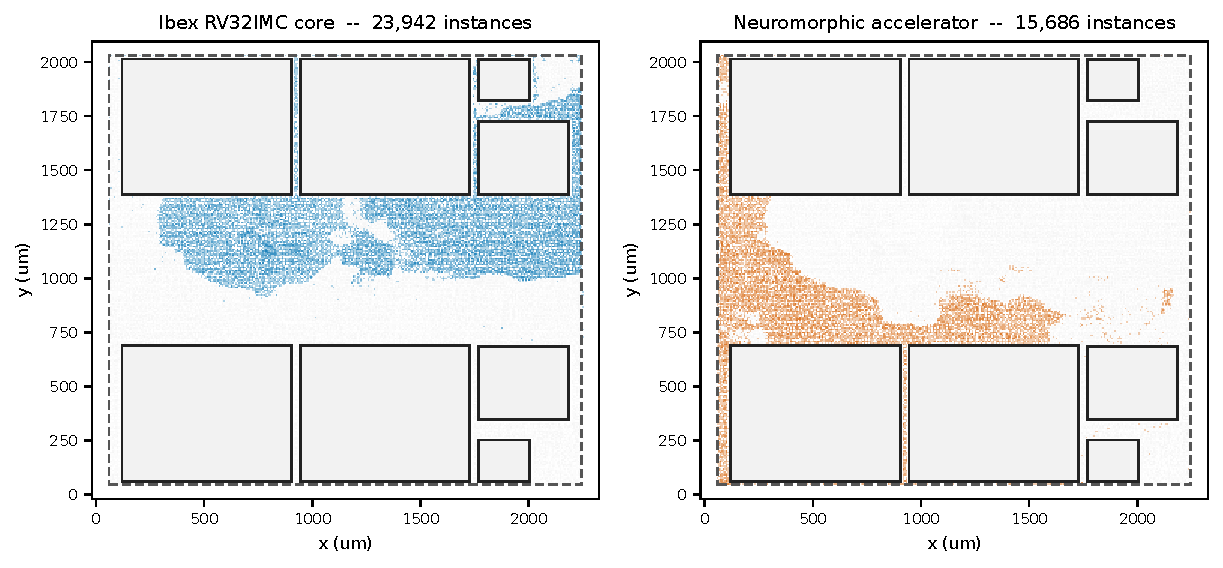
\includegraphics[width=\linewidth]{figures/layout_ibex_npu.pdf}
\caption{The two large blocks of the placed and routed
\code{soc\_top}: the Ibex core (left) and the neuromorphic accelerator
with the frozen die inside it (right), drawn against the same die
outline, core box and eight fixed vendor macros. Generated by
\code{thesis/figures/\allowbreak{}make\_layout\_figures.py} from a
sign-off run's placement database and netlist, which is the only
provenance that script records.}
\label{fig:npu-layout}
\end{figure}

\Cref{fig:npu-layout} answers ``where is the accelerator'' on a placed
and routed layout of the whole system-on-chip, and it must be read with
its method in mind. The die carries 168,592 instances --- the
attribution file the same script writes totals 168,584, a difference of
eight --- and after this flow's synthesis only 1,140 of those instance
names carry a dot at all, 632 of them the RAM's, with exactly one
passing the script's own top-level-block prefix test. A picture that
coloured only the named instances would colour one cell and answer the
question wrongly. Everything else is attributed by connectivity: nets
keep the hierarchical names Yosys did not create, so every net that
still carries a top-level prefix votes for that block; each anonymous
cell takes the block most of its pins' nets vote for; and two rounds of
neighbour propagation resolve the rest.

\textbf{The error bar is published with the picture and is 9.75\,\%.}
Of the 60,694 instances that are not fill, decap, tie or antenna cells,
5,916 could not be attributed and are drawn in grey rather than hidden;
107,890 fill, decap and diode instances are not drawn at all
(\code{thesis/figures/\allowbreak{}layout\_attribution.json}). The
accelerator's share is \textbf{15,686 instances} against the Ibex
core's 23,942 --- 25.8\,\% and 39.4\,\% of those 60,694.

The picture shows a block the placer spread rather than clustered: the
accelerator's cells occupy the lower half of the central channel
between the two macro rows, with the core taking the upper half, plus a
column running the full height of the die down its left edge. Apart
from the eight fixed macros, nothing here was told where to go.

It is also the physical statement of what the area measurements said.
At \dcite{51}{section 11}, on Yosys statistics against the
typical-corner library, the connection alone with the die black-boxed
was 2,723 cells and 57,805.4988 square micrometres and the whole
subsystem including the die was 12,421 cells and 209,739.0834 ---
\textbf{76.08\,\%} of the Ibex reference of 275,682.6198 by cell area.
Two hardening waves superseded those rows: the same recipe in
\dcite{56}{section 7} gives \textbf{3,416 cells and 67,338.0540} for
the connection and \textbf{13,148 cells, 2,092 flip-flops and
219,294.8478} for the whole subsystem. More than half of the connection
is its two event queues --- 53.5\,\% by area at the earlier measurement
--- expensive because they carry entry parity, pointer voting and drop
counting.

\section{What is open}

There is no second node and no router, so the mesh link is a frozen
interface with no implementation, and there are no descriptor rings
--- a ring would be a third bus master on a fabric whose fairness
property is written for two. Multi-pass sequencing is exercised by the
pilot's own suite and by nothing on the system-on-chip, where the tile
offset is written once, to zero. The weight path still enters the node
one register at a time, because that is the die's only weight port; the
flash controller changed where the words come from, not how they enter
(\dcite{51}{section 14}, corrected 2026-09-05).

Most of the connection's flip-flops are unprotected by decision --- the
transport's shift register, the engine's state, the window's captured
request and the frame guards --- and the queues' stored words carry
\code{aer\_fifo}'s detect-only entry parity and nothing beyond it. In
both cases the reason is a measurement rather than a budget. That queue
storage is 37.6\,\% of the connection's flip-flops now that the block
has grown, was 41.2\,\% when the campaign measured it, and is 53.5\,\%
of the area \dcite{51}{section 11} reports; it produced zero silent
wrong inferences in 100 draws, because occupancy is low and most of
those bits are storage nothing will read: a wave that started with the
biggest structure would have bought nothing. The largest site now left
is the engine's state register, at 7 of 20, which
\cref{eq:h5} has made load-bearing for a pin it was only implicitly
related to before.

One limit applies to everything measured here: every campaign in this
chapter is register-transfer, single-bit and flip-flop-only. No
back-annotated timing, no multi-bit strike, and no single-event
transient in combinational logic \cite{shivakumar2002} --- which matters because the strobe
gate \emph{is} combinational logic, so a transient on it is a failure
mode no instrument here can see. A gate-level netlist carrying the
connection has since been injected into --- \dcite{82}{} draws into the
accelerator's gated domain on a placed layout --- but at zero cell
delay and under a workload that never touches the accelerator
(\dcite{82}{section 8}).

\chapter{Radiation hardening}
\label{ch:harden}

\section{The criterion, and why it is not the flip-flop count}
\label{sec:harden-criterion}

Nothing here is protected because it sounds important. The ranking was
written once, in \dcite{41}{section 3.1}, and every wave since has
applied it unchanged. \textbf{What rewrites this register?} One the
block overwrites every tick sheds an upset on its own; one written once
in a mission keeps it for the mission. \textbf{Does its corruption
announce itself?} A part that resets too early is wrong and loud; a
watchdog that has quietly stopped being a watchdog is wrong and silent,
and the system believes it still has one. Everything persistent
\emph{and} silent is protected; everything the block rewrites is not.

That is close to the inverse of the flip-flop count, and the inversion
has been measured four times. In the watchdog, \code{counter},
\code{reload} and \code{pre} are 36 flip-flops against the protected
word's 22 and get nothing (\dcite{41}{section 3.3}). In the boot block,
\code{BRPT} and \code{EPOCH} are 64 of 92 flip-flops with zero boot
consequence (\dcite{69}{section 1}). And in the accelerator's connection the
two queue strata are \SI{41.2}{\percent} of the flip-flops and
contribute \emph{zero} to the measured corruption rate
(\dcite{52}{section 6.3}).

In build order: triple modular redundancy over bundled decision state;
a single-error-correcting, double-error-detecting (SECDED) code over the
register file, over the time base, and, shortened, over both memories,
each with a scrub; redundancy over the boot decision word; and clock
gates designed so that a sleeping block can still report an upset. Each
was measured against the design without it, and three measurements came
back negative.

\begin{figure}[tbp]
\centering
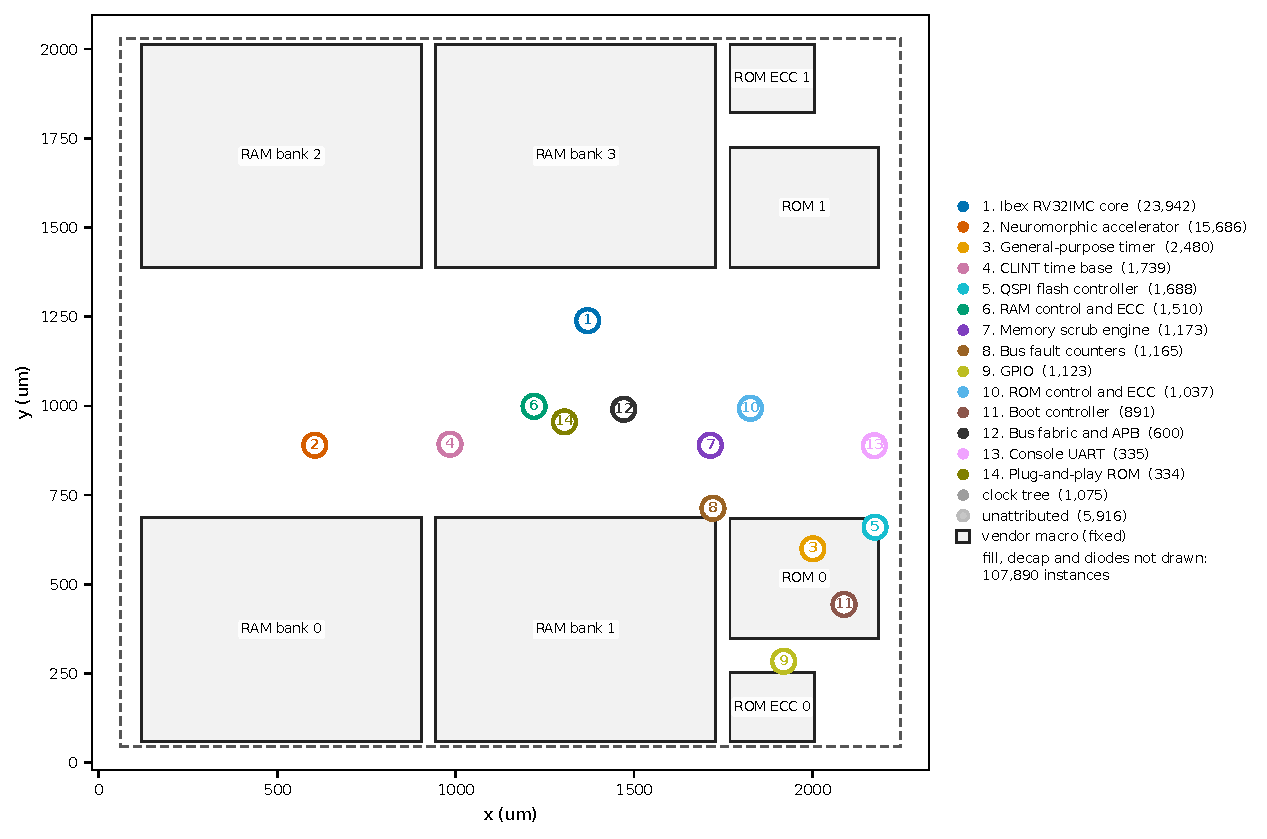
\includegraphics[width=\linewidth]{figures/layout_blocks.pdf}
\caption{Every standard cell of the placed die, coloured by block. Only
about \num{7700} instances still carry a hierarchical name after
synthesis, so attribution is by connectivity --- nets keep their names,
each anonymous cell takes the block most of its pins' nets vote for, and
two rounds of neighbour propagation follow
(\code{thesis/figures/make\_layout\_figures.py}, whose docstring counts
\num{168592} instances where its output file counts \num{168584}; these
figures are the output file's). The remainder, \num{5916} cells or
\SI{9.75}{\percent} of the \num{60694} non-fill cells, is drawn grey
rather than hidden. The protection's own logic is five legend entries
--- RAM control and ECC (\num{1510} cells), the scrub engine
(\num{1173}), the bus fault counters (\num{1165}), ROM control and ECC
(\num{1037}), the boot controller (\num{891}) --- about
\SI{9.5}{\percent} of the non-fill cells [estimate, arithmetic on the
legend].}
\label{fig:harden-blocks}
\end{figure}

\section{Triple modular redundancy, and why one bit cannot have it}
\label{sec:harden-tmr}

Three copies of a flag cannot be held apart. \code{hw/rtl/pilot\_top.v}
section 8.2 proves it: over one bit there are exactly two storage
functions, $x$ and $\lnot x$, so a third replica is bit-for-bit
identical to one of the others and Yosys's \code{opt\_merge} hashes it
away. Over $W$ bits the affine transforms give $2(2^W-1)$ coordinate
functions where three replicas need six, so \textbf{three bits is the
first width at which a third replica has a function left to take}
(\dcite{30}{section 3.3}; \dcite{41}{section 4.1}). Six of the watchdog's eight protected fields
are one bit wide, and replicating one naively yields a single flip-flop
with a voter voting it against itself --- while \textbf{every functional
test and every proof here would still pass}. Polarity cannot rescue it either
(\dcite{33}{section 5}).

So the bits are concatenated into one word and the word is replicated.
Replica A stores $v[i]$, weight 1; B and C store
$\mathrm{enc}_i(v) \oplus \mathrm{POL}[i]$, weight two or three, with
$\mathrm{POL_B} = \lnot\,\mathrm{POL_C}$ --- separated from A because no
function of weight two or more equals $v[i]$ or $\lnot v[i]$, and from
each other by the masks (\dcite{41}{sections 4.2 and 4.3}). The voter is
\code{hw/rtl/tmr\_voter.v}, read in place and never copied, so the SoC's
majority gate is the one \code{formal/tmr\_voter.sby} proves
exhaustively.

\textbf{The bank has no write enable, and that is the scrub.}
Everything in the watchdog is in the power-on reset domain by
requirement W4, so ``written once'' means for the mission, and a bank
that held its value would mask the first upset and then wait for a
second it could not correct. The whole word is therefore written from
the voted value on every clock edge: \textbf{the voter is a continuous
scrubber, and exposure to a second independent upset is one clock cycle
rather than the rest of the mission} (\dcite{41}{section 5.1}). That
bounds accumulation over \emph{time} and nothing else: the header
carries a dated correction saying so, because \dcite{79}{section 1}
measured replicas of this shape sharing rows and abutting.

The watchdog protects eight fields, 22 bits, later 29 when \dcite{43}
added a windowed mode and a kick budget. Worst is \code{dis\_q}, the
bootstrap latch whose corruption sets \code{armed} low so the block
stops for ever; then \code{nmi\_pend}, whose loss means stage 1 never
becomes stage 2, so the watchdog warns for ever without acting
(\dcite{41}{section 3.2}). The report fields are \emph{inside} the
word, because \dcite{16}{section 5.8} had measured this repository's own
safety-net report being the single point of failure: an upset could
erase the announcement of the event it caused.

The ladder the word governs escalates in three stages
(\code{hw/soc/rtl/soc\_wdog.v}, W3): a non-maskable interrupt with one
full timeout for software to notice; then, on a second expiry with the
first unacknowledged, \code{rst\_req\_o} for \code{RST\_CYCLES}, which
the core cannot prevent; then, after \code{ESCALATE} resets since
power-on, an external pin latched until power-on reset, because
resetting has demonstrably not worked and the decision belongs outside
the chip.

The identical bank protects three structures: the watchdog's word at 29
bits, the boot block's at 23 (\dcite{69}), the accelerator connection's
cause bank at 25 (\dcite{55}, widened by \dcite{56}).
\dcite{75}{section 3.3} re-measured all nine replicas by the voter's
fan-in cone, in the block synthesis and in \textbf{every one of the 65
whole-SoC netlists the working tree has kept}, and found $29/29/29$,
$23/23/23$ and $25/25/25$, every set of three disjoint.

\section{The register file}
\label{sec:harden-regfile}

The core's campaign ranked its structures by what their corruption costs
and the answer was unambiguous: the register file is 992 of the core's
\num{2198} injectable RTL bits --- \SI{45}{\percent} --- and carries 3.2
of the 4.9 design-weighted percentage points of wrong-or-dead outcome,
more than everything else in the core combined
(\code{hw/soc/rtl/ibex\_regfile\_secded.v} header, citing \dcite{42}).
That file carries upstream's module name and port list and is given to
the build instead of upstream's own, so the Ibex checkout stays a
pristine clone at the pinned commit; the cost, recorded rather than
glossed, is that an upstream port whose \emph{meaning} changes without
its name changing is caught by nothing (\dcite{43}{section 3.2}).

The codec is \code{hw/rtl/secded\_enc.v} and \code{secded\_dec.v}, read
in place and fixed at 72 bits over 64 --- \emph{one} codec on the die,
which is the objection \dcite{38} raised against lockstep's second one.
One codeword per register with the upper 32 data bits tied off gives the
$(40,32)$ shortening; then one check row is identically zero over a
32-bit field, so the optimiser deletes one flip-flop per register, 31 in
all, and what remains is $(39,32)$, \textbf{the minimal SECDED width for
32 data bits}. The netlist census counts 217 check flip-flops and
would fail at 248 (\dcite{43}{section 6.3}).

Correction on read alone leaves the corruption in the flip-flop, and a
register held across a long call keeps it as long as it holds its value
--- \textbf{the second upset in that word is uncorrectable}. So a
pointer walks \code{x1}\dots\code{x31}, decoding and re-encoding one
register per idle cycle; when the core writes, the scrub stalls and the
pointer holds rather than skipping. The period is \textbf{not proved
bounded}: 31 cycles when the core is idle, unbounded in the limit of a
program that writes the file every cycle for ever
(\dcite{43}{section 6.4}).

At first nothing could read the module's correction counters, because
adding an error output is a patch to \code{ibex\_top.sv}. So
\code{opt\_clean} deleted them and the report cost zero area, with a
test asserting that it did --- \emph{a test whose failure would be the
good news} --- and in silicon a corrected upset and no upset were the
same event (\dcite{43}{section 6.5}). \dcite{44} closed that with three
anchored hunks applied to a \emph{generated} copy of
\code{ibex\_top.v}, never committed, routing the line to
\code{soc\_busstat.v}, demonstrated with a load instruction rather than
a hierarchical read: all four of the core campaign's \code{x23}
records end with the golden answer and with software reading
\code{CNT\_RFSEC = 1}.

It does not protect the addresses --- a corrupted \code{raddr} reaches
the wrong register with a perfectly valid codeword --- nor the other
\SI{55}{\percent} of the core, which carries the highest per-bit rates
in the design.

\section{The time base}
\label{sec:harden-mtime}

\code{mtime} was ranked first for protection by three documents and
protected by none, for the same reason each time: an upset in it is
persistent and silent --- it displaces the architectural clock for ever
--- but it cannot disarm anything, so the backstop went first
(\dcite{58}{section 1}).

The answer is not replication, because a counter has structure a general
register does not. \code{mtime} is the 64-bit data field of a $(72,64)$
codeword whose eight check bits are the only added state. Every tick the
stored word is decoded; the corrected value is what increments, what the
comparator sees and what a bus read returns; and \textbf{the check bits
are re-encoded over the value that goes back in, not over the value that
was stored}. That clause is the whole design: encoding over the stored
value builds an ECC counter that silently does nothing, the code
following the corruption into consistency on the next edge
(\dcite{58}{section 3.1}). Since the word is rewritten every clock the
scrub period is one cycle, so there is no scrubber to build and no
accumulation to bound.

Six designs were synthesised against one baseline
(\dcite{58}{section 4}) and two results are negative. \textbf{The
residue-mod-3 detector that \dcite{41}{section 7.4} proposed as the
cheap answer costs \SI{98.694}{\percent} of what the corrector costs and
corrects nothing}: the cost of any check over a 64-bit counter is the
reduction tree that recomputes it, not the shadow register, so the
flip-flop count, 2 against 8, is not where the money is. And
\dcite{41}'s unsynthesised estimate for replicating \code{mtime} and
\code{mtimecmp} --- ``roughly \SI{27000}{\micro\meter\squared} \dots\
256 more flip-flops'' --- measured at
\SI{25792.0740}{\micro\meter\squared} and \emph{exactly} 256 flip-flops,
\SI{4.68}{\percent} high; a good estimate, recorded as one. The code
corrects the same 64 bits for \SI{50.224}{\percent} of the area of
replicating them.

Two decisions follow the same criterion. That 11 of the 64 bits are
architecturally dead over a five-year mission is an argument \emph{for}
covering them, since deadness bounds the fault-free value and not the
faulty one --- truncation saves \SI{1438.1766}{\micro\meter\squared} and
is ``not a protection; a cheaper failure''
(\dcite{58}{section 4.5}). And \code{mtimecmp} gets nothing: software
rewrites it every deadline, and its worst direction is a missed
deadline, the exact failure the watchdog backs up. The cost that is not area: the CLINT's bounded check went from
\SI{6}{\second} to 18\,min 19\,s and its $k$-induction proof from
\SI{2}{\second} to 5\,min 57\,s, because eight XOR reductions of weight
26 over a 64-bit counter is a hard SMT problem in a way a 22-bit voted
word is not (\dcite{58}{section 9.3}).

\section{The memories}
\label{sec:harden-mem}

\SI{72}{\kibi\byte} of RAM and ROM was long the largest storage with
nothing checking a word read out of it. \dcite{58} expected an easy fit,
because the codec is $(72,64)$ and the RAM macro's row is 64 bits.
\textbf{That coincidence is the problem}: a $(72,64)$ codeword is eight
bits \emph{wider} than the row, and a hard macro has no bit-widening.
Six options were costed from the vendor LEF; keeping
\SI{64}{\kibi\byte} needs a seventh macro at
\SI{+491633.62}{\micro\meter\squared} or
\SI{+257608.51}{\micro\meter\squared} \emph{and} a read-modify-write on
every sub-word store, which is a change to the bus protocol rather than
a wrapper (\dcite{67}{section 3}).

What was built puts the check bits in the row and halves the RAM. A
32-bit word is stored as \textbf{four $(16,8)$ byte codewords}, each the
same Hsiao code with 56 data bits tied off, shortening to the minimal
SECDED width for a byte; four of them is exactly 64 bits, so there is no
seventh macro, no die growth and no read-modify-write, a byte write
landing through the macro's own per-bit write mask with its check bits
beside it. \textbf{The RAM is \SI{32}{\kibi\byte}, not
\SI{64}{\kibi\byte}}, a halving the bring-up program does not notice
because it uses \textbf{192 bytes} of static data plus a stack. An
uncorrectable syndrome answers the read with a bus error, so \textbf{the
recovery is a trap, not a wrong word}.

A word the program never touches is rewritten never, so the memories
need a scrubber, and a bus master would have been a re-proof of a fabric
whose arbiter is written for two. This one lives behind the row port: in
an idle cycle it reads a row; in the next,
if the bus is still not asking, it writes back only the lanes the
decoder corrected; if the bus asks, the bus has the port and the result
is dropped. \textbf{Nothing is ever withheld from the bus}, which is
proved, and a lane reported uncorrectable is \emph{never} written back,
since re-encoding a wrong byte would turn a detected double error into a
valid codeword over a wrong value --- two of the suite's eight mutations
being exactly those failures (\dcite{67}{section 4.3}).

The interval ships at 255 idle cycles, walking the 8192-row RAM in about
2.1 million idle cycles [estimate]. The campaign found the bound that
matters and it is not the expected one: at interval 0 the scrubber
repaired 135 of 360 injections against 36 at the shipped setting ---
\emph{and missed what the slower walk caught}, because the pointer had
left the program's low rows within the first hundred cycles and did not
return inside the run. \textbf{A scrubber's coverage of a row is the
interval between two visits to it}, which is why the interval is a
register (\dcite{67}{section 7.3}).

Placed on the same die the codec costs \SI{+3.01}{\percent} of
standard-cell area, with the die not one database unit larger and hold
closed at three corners. The timing is the honest half. Pre-layout the decoder fit on the read return with
\SI{+2.0352}{\nano\second} of slack; \textbf{post-layout it does not,
and that margin is what layout spent}. The routed path from a macro's
\code{A\_DOUT} to its capturing flip-flop grows from
\SI{12.7286}{\nano\second} to \SI{14.0728}{\nano\second}, and that
group's violating population from \textbf{68 endpoints to \num{1080}}.
Its endpoint is inside the register file: a load's data now crosses the
memory decoder \emph{and} the register file's own SECDED encoder in one
cycle --- \textbf{two independent codes over one word}, which this
project would not have chosen deliberately, and which is still not the
binding path (\dcite{67}{section 5.3}).

\section{Boot}
\label{sec:harden-boot}

Protecting a memory creates a problem at power-on. An SRAM powers up
undefined and \textbf{so does its check field}, so a word nothing has
written is 32 random data bits beside 32 random check bits, and the
codec's answer is an uncorrectable, answered with a bus error
(\dcite{68}{section 4.1}).

\code{boot\_crt0.S} sweeps the whole RAM before the stack pointer is
set, because the loader's own stack, \code{.data} and \code{.bss} are
inside what it is initialising. And it writes \textbf{whole words}: a
byte store makes one of a row's four codewords valid and leaves three as
the SRAM powered up, so ``initialise the RAM'' is not the requirement
--- ``write whole codewords'' is. Both counterfactuals time out at
\num{900095} cycles with a double fault: the loader faults on the first
RAM word nobody wrote, and \emph{the trap handler reads a word nobody
wrote too}. The byte sweep is the instructive one,
leaving \num{1648} uncorrectable rows against no sweep's \num{1706}
while looking initialised (\dcite{68}{section 4.4}). The sweep costs
\num{49178} cycles, \textbf{6.003 per word}, \SI{26.5}{\percent} of the
boot; the image checksum is then computed \emph{from the RAM} rather
than the flash, so a word that arrived intact and landed on a row whose
codeword did not take is caught.

The boot block is 92 flip-flops and \dcite{69} protects \textbf{eighteen}
--- the boot counter, the sampled straps, the watchdog-pin readback, two
validity bits, the sampling delay, and one the campaign added. That one
is the finding. \code{sys\_q} was ranked unprotected because it is
rewritten from \code{rst\_ni} every clock --- true of the register,
false of the consequence, since an upset there manufactures a release
edge, the boot counter increments, and \textbf{the counter is saturating
and power-on-only, so nothing ever takes it back}. Three of four draws
came back as silent corruption and one put the part past its attempt
limit for the power cycle, so it moved into the protected word at a cost
of two flip-flops (\dcite{69}{section 8.4}).

\section{Stopping the clock without losing the report}
\label{sec:harden-clock}

Power, not frequency, is the requirement this design is written against:
\dcite{57} measured \SI{33.890}{\milli\watt} computing and
\SI{5.539}{\milli\watt} waiting at the typical corner, against a
\SI{34.835}{\milli\watt} sign-off figure taken with no switching
activity. \dcite{76} then added two clock gates, and the interesting
part is what gating a fault-tolerant block gets wrong by default. \textbf{A
clock-gated flip-flop still holds state and can still be upset; what it
cannot do is report the upset}, because the voter's correction, the
queue's parity discard and the cause bank's mismatch are all recorded by
registers that need a clock. A sleeping accelerator would have absorbed
the upset and told nobody --- the defect \dcite{52}{section 10} named
and \dcite{55} closed. So all eleven fault lines are terms of the
accelerator's clock-gate enable: \textbf{an upset inside a sleeping
block wakes it up}, at zero cycles of latency, because the enable is
combinational and an integrated clock gate latches it on the falling
edge (\dcite{76}{section 3.2}).

The negative result is that neither clock-gating check closes at the
slow corner --- \SI{-0.7495}{\nano\second} for the fabric's gate and
\SI{-5.0198}{\nano\second} for the accelerator's --- and a violated
setup check at a clock gate is a possible glitch on a clock net, a width
this project has no instrument to measure. \dcite{76} blamed the eleven
fault lines and ranked their removal first; \dcite{77} cut the launch
domains one at a time on that netlist and found the worst path starting
\emph{inside} the accelerator, where every fault line starts, at only
\SI{-1.3129}{\nano\second}, the \SI{-5.0198}{\nano\second} launching
instead from \textbf{the register-file read address that gives the whole
design its worst slack}. The repair was built anyway, for a better
reason: the enable is split by \emph{arrival}, and a term that is a
function of registers the clock has stopped cannot pulse and vanish, so
the cost is \textbf{one cycle of wake latency on a fault and one
flip-flop}, proved rather than hoped (\dcite{77}{sections 1, 3 and 6}).

\section{W9: a correction that cost a reset}
\label{sec:harden-w9}

The sharpest result in the corpus came from measuring the netlist
instead of the RTL. In a gate-level campaign on the watchdog's three
replica banks, \textbf{174 of 174 injected upsets classified CORRECTED
--- and every one of them reset the SoC one clock later}
(\dcite{74}{section 10.2}).

The mechanism is a decode. \code{rst\_req\_o} was
\code{(rst\_hold != 0)}, a five-input OR-reduce of bits 21:17 of the
\emph{voted} word, and two of the three replica outputs are
\code{mix\_dec} of their stored bits --- an XOR tree over all 29
flip-flops of the bank. \code{soc\_top.v} then built
\code{rst\_raw\_n = rst\_ni \&\& !wdog\_rst\_req} and hung the SoC's
reset synchroniser off it \emph{asynchronously}, under a comment reading
``rst\_req is a registered signal in this clock domain''. It was not.
\textbf{The consumer documented the assumption and the producer did not
meet it}, and nothing checked it (\dcite{75}{section 5.1}).

That this is a hazard rather than an intended decode needed no
simulation. Grouping every flip-flop's reset net by the set of
flip-flops feeding it combinationally, the signed-off netlist has
\textbf{five distinct asynchronous-reset source sets}: four are a port
or one or two \emph{registered} signals, and a flip-flop's output does
not glitch. The fifth is \code{rst\_raw\_n}, whose combinational fan-in
is \textbf{25 flip-flops of the three replica banks and nothing else}
(\dcite{75}{section 6}).

The fix is one flip-flop. \code{in\_reset\_q} is the same predicate
computed from the \emph{pre-storage} word rather than the decode, so the
two are equal on every cycle --- proved by $k$-induction as W9a --- and
\code{rst\_req\_o = in\_reset \&\& in\_reset\_q}. The masking is
logical rather than structural, so the mapper may factor it freely; that
it survived mapping is proved by SAT on the mapped cells, with two
mutations that make the proof fail, one of which keeps the flip-flop and
the cell count and gets the logic wrong (\dcite{75}{section 7.4}). It
cost \textbf{one flip-flop} and \SI{+643.0536}{\micro\meter\squared} on
the whole SoC, with no die area, no hold margin at any corner and no
DRC; a block-level area figure was published and then
\textbf{withdrawn} on 2026-09-09 because it did not reproduce under any
of nine recipes, and it is not quoted here.

\begin{table}[tbp]
\centering
\small
\caption{Resets per corrected upset: 174 injections into the same 87
bits at the same 174 cycles, on four netlists mapped on four separate
occasions (\dcite{75}{section 8.5}). The row is the design and the
column is nothing. In all four the vote behaved identically: 174
\textsc{corrected}, one mismatch cycle each, and even \emph{which}
twenty replicas held their corrupted value rather than being rewritten
--- 4, 8 and 8 by bank --- are the same.}
\label{tab:w9}
\begin{tabular}{lcc}
\toprule
 & unrepaired & repaired \\
\midrule
placed and routed layout & $174/174 = 1.0000$ & $0/174 = 0.0000$ \\
synthesis netlist & $174/174 = 1.0000$ & $0/174 = 0.0000$ \\
\bottomrule
\end{tabular}
\end{table}

\section{The evidence}
\label{sec:harden-evidence}

Every campaign classifies each injection into exactly one of five
classes, decided in this order (\dcite{16}{section 1.6}):
\textsc{hang}, the run did not complete inside its cycle budget
\emph{and} nothing was flagged; \textsc{detected}, a design fault flag
or counter moved; \textsc{sdc}, the output differs from the golden model
and nothing was flagged; \textsc{corrected}, the output matches the
golden model \emph{and} a correction counter moved; \textsc{masked}, the
output matches and nothing moved. \textbf{The golden model decides right
from wrong, always}; the design's own flags only decide whether a wrong
answer was announced.

\textsc{corrected}, rather than ``never \textsc{sdc}'', is therefore the
acceptance criterion for a protected bank, because \textbf{an injection
that never reached a flip-flop comes back \textsc{masked}, and
\textsc{masked} is exactly the quiet nothing a mis-targeted injector
produces} (\dcite{41}{section 8.2}). But it cannot be copied: the
register file's campaign demanded it of every injection and failed at
104 of 124 \emph{on a design that was right}, because a register the
program overwrites before the scrub reaches it has shed the upset
without the codec seeing it. The criterion there is now that nothing is
\textsc{sdc} or \textsc{detected} and every \textsc{masked} record is
\emph{explained} (\dcite{43}{section 9.2}).

\begin{table}[tbp]
\centering\footnotesize
\caption{Fault-injection campaigns bearing on the hardening, with their
paired counterfactuals. Every injection is a single-bit flip into one
flip-flop at a seeded-random cycle inside a measured window.}
\label{tab:campaigns}
\begin{tabularx}{\linewidth}{@{}lr>{\raggedright\arraybackslash}X@{}}
\toprule
Population (source) & $n$ & Result \\
\midrule
Watchdog's own state, RTL (\dcite{41}{\,8.2})
 & 162
 & 126 of 126 into the protected word \textsc{corrected}; 0 SDC, 0 HANG,
   0 disarmed. Later 220 draws at 29 bits: 168 of 168 \\
\quad counterfactual, \code{HARDEN = 0}
 & 32
 & 27 SDC, 1 HANG, \textbf{2 left the watchdog reading disarmed}, 6 of
   32 preserved the escalation order \\
Ibex core, campaign A (\dcite{43}{\,8.2})
 & \num{1400}
 & Register-file strata 0 SDC and 0 HANG in 200, against 3 and 4 before;
   0 uncorrectable syndromes. Design-weighted SDC \SI{2.8}{\percent}
   $\pm$ 1.6 $\to$ \SI{1.3}{\percent} $\pm$ 0.4; HANG
   \SI{2.1}{\percent} $\to$ \SI{0.3}{\percent} \\
Ibex core, campaign AW (\dcite{43}{\,8.4})
 & \num{1400}
 & The window rejected a kick as early on 11 draws, 0 on dead machines,
   and produced \textbf{7 spurious escalations in \num{1232} survivable
   upsets} \\
Supervisor workload (\dcite{46}{\,8})
 & 812
 & 32 of 32 dead machines caught, all by ordinary expiry; the window
   converted 2 silent corruptions into announced failures and caused 2
   of 4 spurious escalations \\
Register file alone (\dcite{43}{\,9.2})
 & 124
 & 107 \textsc{corrected}, 17 \textsc{masked}, 0 unexplained. Without
   the scrub: 99 / 25, of which \textbf{6 unexplained} --- upsets still
   sitting in storage nothing had seen \\
CLINT, hardened (\dcite{58}{\,8.3})
 & 342
 & \code{mtime} 128 of 128 and \code{mtime\_chk} 16 of 16
   \textsc{corrected}; clock displaced 0 times; all 144 announced \\
\quad counterfactual, \code{HARDEN = 0}
 & 326
 & 95 of 128 displaced the clock, worst \num{9223372036854775808} ticks
   --- \num{5845} years at \SI{20}{\nano\second} --- and \textbf{0
   announced} \\
Memories, two builds (\dcite{67}{\,7.2--7.3})
 & 720
 & \textbf{0 SDC, 0 traps, 0 hangs}; 104 corrected at the shipped scrub
   interval (68 on a read, 36 by the scrubber), 168 at interval 0 \\
\quad counterfactual, no check bits
 & 280
 & 17 silent wrong answers, 17 announced failures, 1 hang; \textbf{15 of
   the 17 from one constant} the program reads every round \\
Boot block (\dcite{69}{\,8.3})
 & 572
 & 276 of 276 into the protected word \textsc{corrected}; 0 SDC, 0
   spurious give-up, 0 misreported strap \\
\quad counterfactual, \code{HARDEN = 0}
 & 368
 & 261 SDC; 38 corrupted the boot counter, \textbf{worst by 128 boots};
   11 put the part past its attempt limit, 8 stopped it reaching one \\
NPU connection (\dcite{52}{\,1})
 & 700
 & \SI{4.2}{\percent} $\pm$ 1.6 design-weighted silent corruption; 7 of
   600 killed the machine, and the watchdog caught 7 of 7 \\
Core at gate level (\dcite{74}{\,1})
 & \num{1424}
 & \num{1158} of \num{1175} comparable records classify identically to
   RTL; the register file corrected 171 of 180 \emph{in the gates} \\
Watchdog banks, gate level (\dcite{75}{\,8})
 & 174
 & 174 \textsc{corrected} on each of four netlists --- and
   \cref{tab:w9} \\
\bottomrule
\end{tabularx}
\end{table}

Three entries in \cref{tab:campaigns} are negative results, published as
such. The windowed watchdog was built on a recommendation, proved,
measured, and \textbf{its measured value on the first workload was
zero}: 0 of 30 dead machines caught, 0 of 4 on the records replayed
verbatim, seven spurious escalations bought. The recommendation was
aimed at the wrong failure --- a window fires on a kick that is too
\emph{early}, and the runaway that motivated it was a machine executing
its own instructions in order and petting the watchdog on schedule
(\dcite{43}{section 5.1}). What catches that class is a per-phase kick
budget, 4 of 4 on the same records, and the register file removes the
class at source. On a second workload the window's benefit
(\SI{0.25}{\percent}) and cost (\SI{0.27}{\percent}) are the same size,
and \dcite{46}{section 9} recommends removing it before floorplanning
--- which has not been done, the protected word still being 29 bits in
every netlist censused.

It also costs software a rule rather than hardware area, bounding the
jitter ratio of the program's kick cadence: the original workload
measures \textbf{57.2}, which fits inside no window at all, and the
supervisor written to be what the software will be measures 1.412
time-triggered and 2.104 work-triggered --- \textbf{at which no timeout
at all satisfies both bounds} (\dcite{46}{sections 5 and 7}).

\section{TMR blindness}
\label{sec:harden-blind}

A synthesiser is built to delete deliberately redundant logic, and this
project has been burned by exactly that: \code{pilot\_top.v} section 9
records the configuration TMR merging away entirely, and \dcite{38}
measured \SI{15455}{\micro\meter\squared} of an unguarded lockstep the
mapper was removing. The project's own paper states the general form: a
redundancy claim ``was checked at three levels and was wrong at two of
them''. At the register-transfer level it was true; in the mapped
netlist it was false, structural hashing having collapsed three declared
replicas into one physical bank --- \textbf{and the RTL fault-injection
campaign built to detect exactly that produced bit-identical output on
the defective and the repaired design}, because it deposits into signals
the netlist no longer contains (\code{paper/main.tex}, abstract).

Every functional test here would pass on a netlist with one replica
instead of three, and so would every proof: of five mutations against
the composition proof, the last is the honest negative --- turning the
anti-merge transform off keeps \emph{every} property true, because one
bank answering three times still satisfies them
(\dcite{41}{section 9.4}). \textbf{The only honest place to count
replicas is the netlist.} The census in
\code{sw/tests/test\_soc\_synthesis\_guards.py} is built to be able to
fail: with \code{keep} and \code{keep\_hierarchy} deleted from the
\emph{text} of a scratch copy and the flatten forced, the count does not
move --- 102 then, 132 with the wider word and W9, on two independent
technology mappers --- and the mutations it does fail on are invisible
to everything else, \code{.MIX(0)} on replica C costing 11 flip-flops
and on B and C 22 while being functionally identical RTL, bit for bit at
every port (\dcite{41}{sections 6.2 and 6.3}).

Counting is necessary and not sufficient, and \dcite{75} found out how.
Three instruments answer ``which flip-flops belong to this replica'' and
they disagree. By \textbf{instance path} --- what every guard uses ---
the watchdog's banks are $29/29/29$. By \textbf{Q-net name} they are
$29/14/15$, because the polarity masks make exactly one of B and C reset
to one on every bit, the library has no set flip-flop, \code{dfflibmap}
legalises it as a reset-to-zero flop behind an inverter, and \emph{the
resulting cell is not the cell the name was attached to}. By the voter's
\textbf{fan-in cone} they are $29/29/29$ again. A name is a hypothesis.

And a count of the right size can be a count of the wrong thing.
Changing one argument so the voter reads replica A twice produces a
design that passes \emph{every} check in the repository --- per replica,
total, attribute-free, both mappers, every test, every proof --- and
whose vote is a majority over two distinct values, so an upset in
replica A is not masked at all. The union of the three cones falls from
87 to 58; \textbf{the cone census catches it and nothing else does}, and only if
it anchors on the voter's own input pin rather than the bank's output
wire, which still exists in the mutant (\dcite{75}{section 4.3}). Two
rungs followed: a guard running the cone census over every whole-SoC
netlist the tree has kept, since nothing had ever censused the netlist
the foundry would receive; and \code{formal/eqy/}, which checks that the
netlist computes the RTL's \emph{function} for \code{tmr\_voter} --- the
module a flip-flop census structurally cannot check, having no
flip-flops --- with two negative controls whose passing the Makefile
treats as an error (\dcite{79}{section 2}).

The last rung is the die, and there the claim does not survive intact.
On the frozen pilot's sign-off layout the banks are not
placement-separated: minimum cross-replica separation is
\SI{3.78}{\micro\meter} centre-to-centre, the floor for two cells in
adjacent rows, and 49 pairs abut. Against a null model shuffling only
the replica labels over the same placed positions the banks are
indistinguishable from an arbitrary labelling --- $110.73 \pm 8.26$
expected, 103 observed --- so the finding is not that the placer drew
them together but that \textbf{it did not keep them apart}. What is
measured as a mechanism is a \textbf{4.12-fold concentration on
corresponding bits}: median \SI{27.52}{\micro\meter} against
\SI{113.47}{\micro\meter} over all cross-replica pairs, the shape a
shared voter's wirelength would leave. The same picture appears on
\code{soc\_top} across all three of its TMR structures and two
independent hardens (\dcite{79}{sections 1.2--1.6}).

The limit is carried here unchanged from \dcite{79}{section 3}.
\textbf{A distance is not a safety argument in either direction.} No
single-event cross-section or LET threshold for this process was
measured and none is available; the measurement establishes that this
layout \emph{permits} a common-mode upset over much of the protected
word and says nothing about whether one occurs at any fluence.
``Because the replicas are a few micrometres apart, one ion track
defeats the vote'' is therefore forbidden: it silently supplies a
conversion this work does not have. What it does change is the prose ---
every unqualified sentence saying the configuration is protected by
triple modular redundancy must read \emph{triplicated in the netlist}.
The measurement does not make those sentences false; it removes their
evidence. No placement constraint was applied, and the one time
placement was constrained here the region form did not route and the
manual form cost about \SI{7}{\nano\second} of worst slack.

\section{What it costs}
\label{sec:harden-cost}

\begin{table}[tbp]
\centering\footnotesize
\caption{Measured area of each mechanism, against a baseline measured in
the same session with only the thing being priced turned off. Gate
equivalent is \code{sg13g2\_nand2\_1} $=$
\SI{7.2576}{\micro\meter\squared}; the Ibex reference is
\SI{275682.6198}{\micro\meter\squared}. Deltas are arithmetic on two
measurements [estimate]; every measured row is [fact]. Rows marked
$\dagger$ are deltas on the whole SoC rather than on one block.}
\label{tab:harden-area}
\begin{tabular}{@{}lrrr@{}}
\toprule
Mechanism & $\Delta$ flops & $\Delta$ area (\si{\micro\meter\squared}) & of Ibex \\
\midrule
Watchdog TMR, W6 (\dcite{41}{\,6.5}) & $+49$ & $+5{,}091.0552$ & $+1.85\,\%$ \\
Windowed mode and kick budget (\dcite{43}{\,7.3}) & $+29$ & $+4{,}904.0964$ & $+1.78\,\%$ \\
SECDED register file (\dcite{43}{\,7.1}) & $+222$ & $+38{,}050.5762$ & $+13.80\,\%$ \\
\quad of which the scrub, module alone (\dcite{43}{\,7.2}) & $+5$ & $+9{,}963.5130$ & --- \\
\code{mtime} SECDED, H6 (\dcite{58}{\,7}) & $+8$ & $+7{,}026.8310$ & $+2.549\,\%$ \\
\quad its report in BUSSTAT & $+18$ & $+1{,}917.4050$ & $+0.695\,\%$ \\
Boot decision word, B1 (\dcite{69}{\,1}) & $+51$ & $+5{,}255.9010$ & $+1.9065\,\%$ \\
Memory ECC and scrub engine$^{\dagger}$ (\dcite{67}{\,5.1}) & $+234$ & $+31{,}391.3124$ & --- \\
W9, registered reset request$^{\dagger}$ (\dcite{75}{\,1}) & $+1$ & $+643.0536$ & --- \\
Registered clock-gate wake$^{\dagger}$ (\dcite{77}{\,1}) & $+1$ & $+829.4454$ & --- \\
\midrule
\emph{Declined:} lockstep, for \emph{detection} (\dcite{38}{\,8.5}) & --- & $+309{,}550$ & $+112\,\%$ \\
\emph{Declined:} TMR over \code{mtime}, \code{mtimecmp} (\dcite{58}{\,4}) & $+256$ & $+25{,}792.0740$ & $+9.356\,\%$ \\
\emph{Declined:} residue-mod-3 detector (\dcite{58}{\,4}) & $+2$ & $+6{,}935.0904$ & --- \\
\bottomrule
\end{tabular}
\end{table}

Two habits sit behind \cref{tab:harden-area}, both learned by nearly
getting a number wrong. \textbf{The baseline must be the same source
measured now, with only the priced thing turned off}, never a figure a
previous document published: three waves measured that gap at
\SI{58.17}{\micro\meter\squared}, \SI{25.4394}{\micro\meter\squared}
and \SI{10.9242}{\micro\meter\squared}, the last in the direction that
would have \emph{over}stated the hardening (\dcite{41}{section 6.5};
\dcite{58}{section 7}; \dcite{69}{section 7.1}). And \textbf{a module
measured alone understates what it costs in place}: the register file's
standalone delta is \SI{+31709.55}{\micro\meter\squared} against a
whole-core \SI{+38050.58}{\micro\meter\squared}, \SI{20}{\percent}
larger, because \code{abc} re-optimises across a boundary the flattened
core does not have (\dcite{43}{section 7.2}).

\begin{table}[tbp]
\centering\footnotesize
\caption{Costs that are not area.}
\label{tab:harden-cycles}
\begin{tabularx}{\linewidth}{@{}l>{\raggedright\arraybackslash}X@{}}
\toprule
What & Cost \\
\midrule
Every RTL hardening wave
 & \textbf{Zero cycles.} The whole-SoC self-test reproduced to the cycle
   across each wave: \num{185443} cycles
   (\code{docs/40}--\code{docs/44}), \num{215428}
   (\code{docs/55}--\code{docs/58}), \num{217682}
   (\code{docs/66}--\code{docs/67}), \num{220256} for the program with
   \num{415324} for the run since the boot flow (\dcite{68}{\,8},
   reproduced by \dcite{75}{\,7.5} and \dcite{77}{\,7}). In a fault-free
   machine every decoder is the identity, proved by induction; the
   invariant moves when the program or design gains content, never when
   a protection is added \\
Register-file scrub
 & 31 cycles per sweep when the core is idle; stalls on any cycle the
   core writes; \textbf{period not proved bounded} (\dcite{43}{\,6.4}) \\
\code{mtime} scrub & 1 cycle, by construction (\dcite{58}{\,3.2}) \\
Memory scrub
 & One walk of \num{8192} rows per \num{2100000} idle cycles at the
   shipped interval of 255 [estimate] (\dcite{67}{\,4.3}) \\
Boot RAM sweep
 & \num{49178} cycles, 6.003 per word --- \SI{26.5}{\percent} of the
   boot --- plus 17.01 cycles per word to verify the image out of the
   RAM (\dcite{68}{\,4.2}) \\
Windowed watchdog
 & A bound on the software's kick-jitter ratio,
   $i_{\max}/i_{\min} < 1/(1-2^{-\mathrm{WINS}})$, paid by the program
   (\dcite{43}{\,4.2}) \\
Clock-gate wake
 & Zero cycles as first built; \textbf{one cycle on a fault} after the
   enable was split by arrival (\dcite{77}{\,1}) \\
Register-file read path
 & \SI{2.7928}{\nano\second} at the slow corner, on the module where
   nothing else can move; \SI{0.2593}{\nano\second} recovered for
   \SI{+1201.5486}{\micro\meter\squared} (\dcite{44}{\,5.4}) \\
Memory read return
 & \SI{+1.3442}{\nano\second} routed, that group's violating population
   from 68 endpoints to \num{1080} (\dcite{67}{\,5.3}) \\
Formal
 & The CLINT's bounded check \SI{6}{\second} $\to$ 18\,min 19\,s, its
   proof \SI{2}{\second} $\to$ 5\,min 57\,s (\dcite{58}{\,9.3}) \\
\bottomrule
\end{tabularx}
\end{table}

One line of \cref{tab:harden-cycles} deserves its own sentence, because
the first version of it was wrong. \dcite{43}{section 7.4} attributed a
setup-slack loss and a closure period moving from
\SI{15.98}{\nano\second} to \SI{17.62}{\nano\second} to the register
file's decoder, reasoning that the decoder sits on the read path and the
read path feeds the ALU. \dcite{44} looked at the paths. \textbf{All ten
worst setup paths at the slow corner, in both configurations, start at
\code{cheriot\_enable\_i[0]} --- a configuration input \code{soc\_top.v}
drives with a constant}, which a register-file decoder cannot be on. And
the binding check in the hardened build is not a logic path at all: it
is the \emph{asynchronous reset recovery check} on an unbuffered
\num{2328}-fanout net, with the two hardened builds reporting
bit-identical slacks at every probe. What the protection cost there is
222 more flip-flops on an unbuffered reset net, a place-and-route
obligation and not a logic cost. \textbf{The delta was real and the
attribution was not} (\dcite{44}{sections 5.1 and 5.3}). Consistently
with \dcite{53}{section 9.2} and \dcite{05}{section 4} rule 5,
\emph{no clock frequency is claimed for this design anywhere}; slack
against a \SI{20}{\nano\second} SDC period, with its corner named, is
what is reported.

\section{Four shapes an error takes here}
\label{sec:harden-shapes}

The project keeps a catalogue of the mistakes it makes, because the
shapes repeat and the catalogue is worth more than any single number in
it (\dcite{64}{section 3}; \code{ROADMAP.md} section 3). Four bear on
hardening. They are findings, not apologies.

\paragraph{A green result read wider than what it looked at.}
\dcite{41}{section 6.6} lists eight instances by document and section,
\dcite{43}{section 10} makes it ten, \dcite{58}{section 11} eleven. The
canonical case is the netlist census: it counts flip-flops and asserts
nothing about any other cell, nothing about placement, and nothing about
whether the replicas are \emph{correct}. The fix is never to widen the
claim; it is to build a second instrument at the level the
first cannot see, with a mutation that makes it fail --- which is why
the cone census, the shipped-netlist guard, the equivalence check and
the gate-level campaign all exist. One instance is the shape at its
purest: a mutation harness reported a pass because a build failure
produced no \code{FAIL} lines to parse.

\paragraph{A measured delta attributed to the wrong cause.}
The register file's timing cost is the clearest case: the number moved,
the explanation was wrong, and only looking at the paths found it. The
clock-gate diagnosis of section~\ref{sec:harden-clock} is a second, and
\dcite{61}'s \SI{+4.4}{\percent} estimate --- an earlier absolute area
carried onto a new denominator, measured at \SI{+4.9406}{\percent} by
\dcite{62}{section 1} --- is a third, where the method was the error
rather than the arithmetic. The defence is an
instrument's own resolution: \dcite{44}{section 5.2} measured this
flow's noise floor at about \SI{0.4}{\nano\second} at synthesis, and
\dcite{70} measured it after layout with a control pair that changes
nothing a designer would call a change --- it moves hold by
\SI{0.0198}{\nano\second} and setup by \SI{0.5031}{\nano\second}.

\paragraph{One change leaking in from several places.}
A delta is only a delta if the two runs were asked the same question,
and the answer is a paired counterfactual on identical draws.
\dcite{55}{section 8.3} had to refuse a \SI{19}{\percent} improvement
because its control stratum moved on 15 of 100 records; \dcite{58}
reports its delta because a field-by-field diff over the strata it does
not touch found \textbf{0 of 198 records changed}, and \dcite{69} found
the same zero over 296. \dcite{44} re-ran the entire core campaign and found the two
\num{1400}-record files \emph{byte-identical}, which is stronger than
``the rates agree'', since two records moving in opposite directions
would satisfy that too. The same discipline forced the isolation builds
of \dcite{43}{section 5.4}: with both the window and the budget armed,
both counters have fired by the end of a run that reset itself, and a
report reading them would have credited the window with a catch it did
not make.

\paragraph{The synthesiser deleting redundancy.}
Section~\ref{sec:harden-blind}. The specific hazard is that
\emph{everything else stays green}: the collapsed design satisfies every
property of the composition proof, passes every functional test, and
produces bit-identical fault-injection output. Redundancy is the one
property whose evidence cannot live in the source, because the source is
precisely what the mapper is entitled to rewrite.

\section{What is still open}
\label{sec:harden-open}

\textbf{No radiation data exists for this process.} Neither open PDK
publishes total-ionising-dose or single-event figures, no silicon of
this SoC exists, and no beam time has been taken. Every reliability
number here is a seeded fault-injection measurement on RTL or a placed
netlist, conditional on an upset having landed inside a measured window.
The project has no upset rate $\lambda$ and says so where the arithmetic
would need one (\dcite{67}{section 6.2}).

\textbf{Every campaign is single-bit and flip-flop only}, with no
multi-bit strike and no single-event transient in combinational logic
--- a larger gap for a code than for a replicated bank, because the
code's defence \emph{is} combinational logic, the CLINT's exposed codec
alone being 528 cells (\dcite{58}{section 11}).

\textbf{Addresses are unprotected everywhere}, so a corrupted
register-file address, memory row address or bank select reaches the
wrong location with a perfectly valid codeword, and \textbf{no whole-SoC
campaign reaches a peripheral}. \textbf{The ROM's contents are not
protected in a flight part}: on this PDK the boot ROM is an SRAM that
powers up undefined and nothing in the design can write it, so its check
macros are check bits nobody can initialise; the flight answer is a mask
ROM whose bit is a via and has no stored-upset mechanism
(\dcite{67}{section 8}; \dcite{68}{section 3}). \textbf{And the vendor
macros cannot be signed off on this PDK version}, so neither can the die
that carries them.

% SPDX-FileCopyrightText: 2026 Hasan Melih Akbulut
% SPDX-License-Identifier: CC-BY-4.0

\chapter{Verification}
\label{ch:verif}

\section{Five layers, and the failure they all share}
\label{sec:verif-shape}

The verification programme has five layers: cocotb simulation of blocks
and of the whole system, textual and netlist \emph{guards} that read the
tree without simulating it, SymbiYosys property sets over individual
blocks, an instruction-set proof of the management core against
riscv-formal, and fault-injection campaigns at register-transfer and
gate level. They are five layers and not one because each of them can be
green about something it never looked at, and the corpus has the receipts.
\dcite{41}{section 6.6} says this repository has been bitten eight times
by a green check being read wider than what it examined, and names each
by document. (Two guard files in \code{sw/tests} cite that same section
as listing \emph{nine}; the section itself says eight, and both
statements are in the tree.)
\code{sw/tests/test\_traceability.py}'s own docstring calls its own
rewrite ``the eighth instrument in this tree found to have that shape'',
and \dcite{78}{section 3.2} records the third instance found inside this
project's own guards --- the first one found in a guard written to
prevent the shape.

Four standing rules govern how results are reported, and they are worth
stating before any number. \textbf{Every assert set ships with cover
obligations, and a target with passing asserts and failing covers is
red} (\dcite{09}{section B.1}). \textbf{A bounded result is never
reported as proven}, and every bounded result carries its depth
(\dcite{09}{C.4 item 6}). \textbf{Timing is outside formal scope}, with
OpenSTA the separate authority, so formal results hold for any
timing-clean implementation (\dcite{09}{C.4 item 2}); and \textbf{no
clock frequency is claimed for this design at all}, by
\dcite{05}{section 4 rule 5}, which \dcite{53}{section 9.4} applies to
both of the numbers a layout has reached. Periods, slacks and corner
names are reported where they are measured, in
\Cref{ch:phys}; nothing in this chapter is a frequency. Finally,
\textbf{formal proves mechanisms correct, fault injection measures
architectural sensitivity, and only beam data speaks to cross-sections}
(\dcite{09}{C.4 item 4}) --- so no rate appears anywhere below.

One more convention, inherited from \code{docs/64}: a superseded measurement
is reported as superseded, with its date, rather than overwritten. Two
counts in this chapter are superseded and both are given twice.

\section{Simulation: the cocotb suites}
\label{sec:verif-cocotb}

Counted in the working tree on 15 September 2026: \textbf{33 cocotb test
modules carrying 413 test functions}, across \code{hw/tb} (10 modules,
166 functions), \code{hw/soc/tb/cocotb} (22 modules, 242) and
\code{tt/test} (1 module, 5). They are driven by 30 makefiles, and
\code{scripts/run\_cocotb.sh} reaches all of them: 7 of the 10 under
\code{hw/tb} by default, all 19 under \code{hw/soc/tb/cocotb}, 3 more
modules that share another suite's makefile and are named in the
runner's own table, and \code{tt/test}. The declared-function count is a
floor rather than the number a run reports, because several makefiles
elaborate one module at more than one parameter point:
\code{Makefile.secded} runs the encoder and the decoder,
\code{Makefile.tmr} runs widths 1, 8 and 32, \code{Makefile.scrub} runs
three parameter triples, and \code{Makefile.soc\_pnp} runs two buses.
The last recorded whole-tree run is \code{verification-log.tsv}'s row of
2026-09-11T00:55Z at \code{587fdd8}: \textbf{462 cocotb tests passing, 0
failing, 0 suites not clean}. That row is four days old at the time of
writing and is quoted as what it is.

Three suites are skipped by default and the reason is the freeze.
\code{hw/tb/Makefile.fi} regenerates \code{hw/tb/fi\_campaign\_results.json},
which \code{docs/34} pins by git blob hash for the TTIHP26b submission; running it inside a verification pass rewrote that file's
\code{wall\_seconds} field and dirtied a frozen tree. The campaign is
reproducible on demand and its result is committed, so the runner
declines to re-derive it and says so; \code{RUN\_FROZEN=1} includes it.
The two gate-level suites are skipped for a different reason --- they
need artefacts from a hardening run rather than from the source tree.

\subsection{The runner is itself an instrument, and it has a repair history}

\code{scripts/run\_cocotb.sh} exists because \code{pytest} at the
repository root collects \code{sw/tests} only, so quoting a pytest total
as ``the tests pass'' is wider than what was measured. Four things in it
are the residue of measured defects, and they are worth reading as a
compressed history of how a test count goes wrong.

It \textbf{parses each suite's results XML rather than trusting the make
exit code}, because a cocotb suite can report all tests passing and then
segfault in Icarus teardown --- observed on \code{Makefile.soc\_clint}
and reproducible on committed RTL. That is a tool defect, and the XML is
the evidence that survives it.

It \textbf{refuses to run twice at once} rather than queueing. Counting
is by ``the results XMLs written since this marker'', which orders by
time and not by owner, so two concurrent runs each count the other's
output. On 2026-09-08 two overlapping runs recorded 558 and 624 cocotb
tests for a 401-test repository, and both landed in
\code{verification-log.tsv} looking exactly like measurements; the rows
are still there, superseded by the 22:35Z row for the same commit
\code{1ecf509} with the note
\code{supersedes=two-invalid-rows-for-1ecf509-concurrent-run-overcount},
because a log that quietly loses its own bad measurements is not a log.

The marker is a \textbf{file touched after a pause} rather than a
second-resolution timestamp, and \code{docs/66} measured what the timestamp
version cost: the previous suite's XML, written in the same second the
timestamp was taken, was counted again under the next suite's name, and
\code{soc\_qspi} reported 47 tests for a 16-test suite because
\code{soc\_npu}'s 31 had landed three seconds earlier. The runner also
sums \emph{every} XML written during a suite rather than taking the
newest, because a parameterised suite writes several and taking one made
\code{soc\_gptimer} read 10 on one run and 3 on the next while ``0
failed'' stayed true throughout.

Finally it carries a \textbf{completeness check}: every
\code{test\_*.py} in those two directories must be named by some
makefile or by the runner's own table, and one that is not is an error
at the moment it is added rather than a suite that quietly never runs.
On 2026-09-11 three modules did not run --- \code{test\_aer\_fifo},
whose makefile is named \code{Makefile} and so fell outside the
\code{Makefile.*} glob, and \code{test\_soc\_npu\_defects} and
\code{test\_soc\_wdog\_strap}, each reachable only by typing
\code{MODULE=} by hand. All three were green, all three were invisible,
and an edit re-opening the defect two of them exist to catch would have
passed every check in the tree.

\subsection{What the suites cover, and what only they can see}

The block suites drive a module's ports and check its contract:
\code{test\_soc\_bus} (16 functions), \code{test\_soc\_clint} (17),
\code{test\_soc\_qspi} (16), \code{test\_soc\_wdog} (15),
\code{test\_soc\_gpio} (14), \code{test\_soc\_uart} (14),
\code{test\_soc\_boot} (18), \code{test\_soc\_npu} (35 --- the largest
in the tree). Two of them are \emph{campaigns rather than tests}:
\code{test\_soc\_wdog\_fi} carries 220 injections inside three test
functions and \code{test\_ibex\_regfile\_secded} carries 124 inside six
(\dcite{44}{section 8.3}), which is how the mechanisms' behavioural
recovery is measured on top of the proof of the code. Two more suites
have the same shape for their own blocks: \code{test\_soc\_boot\_fi}
injects into the boot register block's own state, and
\code{test\_soc\_clint\_fi} into the architectural time base's 72 stored
bits, each establishing an unhardened baseline and the delta against it
in the same file.

Three suites exist only to fail against the RTL as it was before a fix
--- \code{test\_soc\_npu\_defects}, \code{test\_soc\_wdog\_strap},
\code{test\_soc\_uart\_defects} --- and their headers document a command
line with \code{MODULE=} on it so they can be run twice, once against
the tree and once against a copy of the pre-fix source. That is why they
share a parent makefile rather than acquiring one each: two places to
keep sources and parameters in step is one place too many.

What simulation sees that nothing below it does is \textbf{a whole
machine executing a program}. \dcite{38}{section 7} runs a self-checking
C program on the sv2v output of Ibex under Icarus with no SystemVerilog
anywhere in the flow: eleven checks covering fetch, the RV32I ALU, every
RV32M operation including the ISA's divide-by-zero results, loads and
stores at three widths, branches, recursion, compressed code, CSR access,
an illegal-instruction trap, and --- test 10 --- PMP enforcement, a
locked read-only NAPOT region permitting a load and faulting a store with
\code{mcause = 7}. All eleven pass in \num{131694} cycles. On the
hardened system the equivalent run is 22 checks, stage~1 at cycle
\num{174128}, the core asleep after \num{185443} cycles, 587 console
characters and 0 framing errors, and \dcite{43}{section 9.1} reports it
cycle-identical to the run before the register file was substituted.
That cycle-identity is the strongest available evidence that a
substitution was transparent --- and \dcite{44}{section 9} is explicit
that it is an expectation and not a measurement, which is why a campaign
was run anyway.

What simulation cannot see is everything the design is that this program
never exercises: one workload, one seed, one parameter point. The gate
level adds a second limit of its own, and it is a tool limit rather than
a design one. The IHP cell models drive their outputs from
\code{delayed\_D}, \code{delayed\_CLK} and \code{delayed\_RESET\_B} ---
the negative-timing-check outputs of \code{\$setuphold} and
\code{\$recrem} --- which Icarus 12 does not implement. Every
\code{sg13g2\_dfrbpq\_1} output then sits at \code{x} and the design
reads back zeros. On the shuttle submission's own suite that is 1 of 5
passing (\dcite{15}{section 5.4}); in \code{hw/tb} it was 21 of 21
failing (\dcite{24}{section 3.1}). Both read exactly like a dead
netlist and neither is one. \code{hw/tb/Makefile.gl} refuses to run
under Icarus 12; \code{tt/test} is frozen and generated and cannot carry
a guard of its own, so \code{run\_cocotb.sh} forces \code{GATES=} on its
command line where it beats an exported \code{GATES=yes}, and applies
the version check on its behalf under \code{TT\_GATES=1}.

\section{Guards: the checks that do not simulate}
\label{sec:verif-guards}

A \emph{guard} in this project is a pytest that reads the tree --- RTL
text, a generated netlist, a flow script, a document, the git index ---
and asserts a property of it. Guards live in \code{sw/tests}, and on
15 September 2026 pytest collects \textbf{526 tests across 25 files}
there. The last recorded whole-suite run is \code{verification-log.tsv}'s
2026-09-11 row at 509 passing, 0 failing, which the count above
supersedes; \dcite{44}{section 8.3} reports 315 at its own writing and
\code{docs/43} closed at 295, and both are left standing as records of their
date. The largest files are \code{test\_doc\_links.py} (96 tests),
\code{test\_soc\_synthesis\_guards.py} (68), \code{test\_lif\_core.py}
(41), \code{test\_synthesis\_guards.py} (40) and \code{test\_secded.py}
(37).

Run whole on 15 September 2026 the suite reports \textbf{523 passed and
3 failed in 881 seconds}, and the three failures are more informative
than the 523. \textbf{Two of them are the suite catching the tree
mid-edit.} A guard that compares the newest formal task count stated in
the index and the roadmap against a count summed from the \code{[tasks]}
sections failed during the run and passes on a re-run minutes later,
because the document it reads acquired its 2026-09-15 recount while the
run was in progress. And the guard asserting that no second copy of the
frozen accelerator source exists under \code{hw/soc} failed on
\code{hw/soc/formal/soc\_npu\_prove/src/pilot\_top.v} --- which is a
SymbiYosys scratch copy, because sby copies every file of a job's
\code{[files]} section into its own working directory. That guard was
repaired the same day, and the repair is this chapter's principle
applied once more: a directory is a solver run directory when it
contains sby's own \code{config.sby}, walked up from the file, because
the run directories are called \code{<job>\_bmc}, \code{<job>\_prove},
\code{soc\_npu}, \code{regfile\_scrub} \emph{and the next job will
invent another spelling}. \textbf{The third failure is real and still
open as this is written}: \code{docs/82} landed on 15 September and is not
yet named in \code{docs/00-index.md}, so the link guard reports it
unreachable from the entry point --- which is the guard doing exactly
what it is for.

Guards exist because, as \code{sw/tests/test\_soc\_npu\_guards.py} puts
it in its own header, the cocotb suite and the formal job check
\emph{behaviour}, and neither can notice that a constant has been copied
instead of generated, that the frozen directory has been written to, or
that the design has grown a second copy of a register map. The boot
guards' header states the placement rule the whole family follows: a
guard belongs at the stage that can satisfy it. \code{soc\_boot.sby}
proves the boot counter is not writable and says nothing about
\code{rst\_ni} on that block being the \emph{system} reset, which is what
makes the counter count boots; \code{test\_soc\_boot.py} drives the
block's ports by hand and says nothing about the ports being connected;
the whole-system run boots and says nothing about the RAM sweep being
first, because on a healthy simulation an unswept RAM is
indistinguishable from a swept one.

\subsection{The principle: check the property, not the name}

The governing discipline is \code{docs/78}'s, and it was learned twice in
that document alone.

\code{scripts/spdx\_check.py} reported itself as licence-tagged when it
carried no header at all. The first version searched the first 4,000
characters for the identifier string, anywhere, in any context --- and
the file's own docstring and its own regular expression both contain
that string, so \textbf{the checker read its own prose as its own
licence}. It went unnoticed because it passed. It surfaced only when an
unrelated edit pushed the docstring past the 4,000-character window and
the file abruptly turned up missing. The repair narrows the property: a
tag counts only on a comment line within the first twelve lines, which
is where a header is and where prose about headers is not.

The second is sharper because it is a guard failing at guarding.
\code{scripts/gen\_public\_mirror.py} had to rewrite one sentence in a
CI workflow before publishing it, and refused to run if the sentence had
changed. It was written as \code{if wf in files:}, anchored on the
\emph{filename} \code{.github/\allowbreak workflows/\allowbreak docs.yml}. When three workflows
were folded into one and that file was deleted, the guard did not fire
--- it was skipped --- and the generator wrote 511 files as though
nothing were owed. \dcite{78}{section 3.2} states the rule that came out
of it: \textbf{a check that cannot fail when the thing it checks is
absent is not a check.} It now raises on absence and anchors on a
paragraph's content rather than on a path.

The same rule decided an anchor in the hardening guards.
\code{test\_soc\_shipped\_netlist\_guards.py} identifies a
triple-modular-redundancy replica by walking the fan-in cone of
\emph{the voter's own input pin}, and \dcite{75}{section 4.3} explains
why the obvious anchor is wrong: anchoring on the bank's output wire
\code{qb} --- the same net in a correct design --- misses the defect,
because in a design where the voter reads replica A twice, \code{qb}
still exists and is still driven by replica B; it is simply not what the
voter reads. The guard tries \code{u\_prot\_vote.in\_b} first, falls back
to \code{qb} only where that name did not survive, and reports which
candidate it used on every row.

\subsection{Three guards that caught something}

\paragraph{The voter wired to one replica twice.} This is the sharpest
of them because every other instrument in the repository passes on the
defect. \code{test\_a\_voter\_wired\_to\_one\_\allowbreak replica\_twice\_\allowbreak is\_caught\_only\_by\_the\_cone}
changes one argument in a scratch copy of \code{soc\_wdog.v} ---
\code{.in\_b(qa)} where the design has \code{qb} --- and
\dcite{75}{section 4.3} measures what each instrument then says
(\Cref{tab:verif-cone}). The \code{(* keep *)} attribute on the bank's
storage keeps replica B's flip-flops in the netlist although nothing
reads them, so the mutant is a design with three intact banks whose vote
is $\mathrm{maj}(q_a, q_a, q_c) = q_a$: \textbf{an upset in replica A is
not masked at all}. Every count in this repository passes on it, every
functional test passes, every proof passes, and the cone census fails.
The shape is named precisely in that section: not an instrument that
undercounted, but an instrument that counted the right number of the
wrong thing.

\begin{table}[tbp]
\centering
\caption{The mutation that only a connectivity census can see: a voter
whose second input is wired to the first replica
(\dcite{75}{section 4.3}). Every flip-flop count agrees; the union of
the three voter-input cones does not.}
\label{tab:verif-cone}
\small
\begin{tabular}{@{}lrr@{}}
\toprule
Check & intact & mutant \\
\midrule
Flip-flops per replica, by instance path & 29 / 29 / 29 & 29 / 29 / 29 \\
Total flip-flops in the block            & 132          & 132 \\
Fan-in cone per voter input              & 29 / 29 / 29 & 29 / 29 / 29 \\
\textbf{Union of the three cones}        & \textbf{87}  & \textbf{58} \\
\textbf{Flip-flops shared by two inputs} & \textbf{0}   & \textbf{29} \\
\bottomrule
\end{tabular}
\end{table}

\paragraph{A fault line that carried a bus signal.}
\code{test\_soc\_clkgate\_guards.py} discharges an assumption that a
proof cannot discharge about itself. \code{hw/soc/formal/clkgate\_wake.sby}
proves a transformation of the accelerator's clock-gate enable from two
side conditions, one of which (its assumption A2) is that the slow half
of the enable is a function of registers that are not being clocked ---
a term that cannot pulse and vanish while the block's clock is stopped.
The guard elaborates the module, flattens it, walks the fan-in cone of
\code{npu\_act\_slow} cut at every sequential cell, and fails if any
input port is reachable. It found \code{C\_INJ\_OVF}, the one fault line
that carries \code{psel\_i}, which the file's own header records that no
reading of the source had noticed.

\paragraph{A guard whose arithmetic was wrong for two widths.}
\dcite{43}{section 9.5} records a latent defect that only a width change
could expose. A synthesis guard asserted that turning the mixing
transform off on both mixed replicas loses $2 \times \mathit{collided}$
flip-flops, where \emph{collided} is the number of bits on which one
polarity mask is zero. At a protected word of 22 bits that is
$2 \times 11 = 22$ and it was right; at 29 bits it is $2 \times 15 = 30$
and the answer is 29. The design was right and the arithmetic was wrong,
and the comment above the assertion had said the right thing all along:
on \emph{every} bit one of the three replicas must collide, because
polarity offers exactly two storage functions per bit and there are three
replicas. The expression is now $\mathit{intact} - \mathit{PROT\_W}$.

\subsection{What guards cannot do}

They read text and netlists, so they catch the ordinary edit and not the
determined one --- the supervisor guards' own header says they cannot
see a watchdog kick reached through a function pointer or an unknown
macro. They compare port \emph{lists} and not port \emph{meanings}: a
port whose semantics changed upstream without its name changing is
invisible to them and to the build, and \dcite{43}{section 3} names that
as an accepted risk. And the netlist guards read git-ignored build
products, so on a fresh clone they skip, with the command that
regenerates the evidence --- and the files say in as many words that a
skip is evidence of nothing.

One guard failure is worth recording because it is the counting layer
failing. Until 2026-09-09 \code{scripts/verify.sh} enumerated formal
results with a two-level glob over \code{hw/soc/formal/*/} and
\code{formal/*/}. riscv-formal does not put its jobs there: its job
directories are four to six levels down under \code{hw/soc/out/}, so the
glob could not reach a single one, and the log recorded
\code{formal\_pass=118, formal\_other=0} for a tree that had 35
non-passing formal jobs in it. The enumeration is now
location-independent by construction --- every directory in the tree
holding both a \code{config.sby} and a \code{logfile.txt} --- and the
verdict is read from sby's own marker file rather than grepped out of
the log, because two jobs died on a configuration error before any
\code{DONE} line was printed and the old code's empty-string arm dropped
them silently: not counted as pass, not counted as other, not counted at
all. The old rows are left standing, and read as what they measured. On
the tree as reported the same day the counts became 425 and 35, and
\code{formal-dispositions.tsv} carries all 35 with a reason and a date:
\textbf{6 FAIL, 3 ERROR, 26 STOPPED}.

\section{The SymbiYosys property sets}
\label{sec:verif-sby}

Counted in the tree on 15 September 2026: \textbf{28 property sets
carrying 137 tasks} --- 8 sets and 54 tasks under \code{formal/} for the
frozen pilot, 20 sets and 83 tasks under \code{hw/soc/formal/} for the
system fabric. \dcite{63}{section 2} states ``87 sby tasks across 16
property sets --- eight under \code{formal/} for the pilot and eight
under \code{hw/soc/formal/}''; that was correct when it was written and
is superseded by the count above, and both are given because the
document is still in the tree saying it. All 54 pilot task directories
carry a \code{PASS} marker. Of the SoC's 83 tasks, 79 have a recorded
workdir: \textbf{76 PASS, 2 TIMEOUT, 1 UNKNOWN}, and the remaining four
have no verdict --- two were stopped by hand and two were still running
when this was written. \Cref{tab:verif-sby} is the complete list.

\begin{longtable}{@{}>{\raggedright\arraybackslash\small}p{0.195\linewidth}
                   >{\raggedright\arraybackslash\small}p{0.245\linewidth}
                   >{\raggedright\arraybackslash\small}p{0.225\linewidth}
                   >{\raggedright\arraybackslash\small}p{0.235\linewidth}@{}}
\caption{Every SymbiYosys job under \code{hw/soc/formal/}, read from the
job headers and \code{hw/soc/formal/Makefile}. Depths are sby depths.
Engines are \code{smtbmc yices} unless named. Results are the verdict
recorded in each task's workdir on 15 September 2026.}
\label{tab:verif-sby}\\
\toprule
\textbf{Job} & \textbf{What it binds} & \textbf{Tasks and depths} &
\textbf{Recorded} \\
\midrule
\endfirsthead
\toprule
\textbf{Job} & \textbf{What it binds} & \textbf{Tasks and depths} &
\textbf{Recorded} \\
\midrule
\endhead
\bottomrule
\endfoot
\code{soc\_bus} & \code{soc\_bus.v}, F1--F9; the decode proved against
the generated \code{soc\_memmap.vh} & bmc 24, prove 12, cover 24 &
3 PASS \\
\code{soc\_apb\_bridge} & \code{soc\_apb\_bridge.v}, A1--A11, clauses of
AMBA 3 APB & bmc 24, prove 12, cover 24 & 3 PASS \\
\code{soc\_apb\_wb} & \code{soc\_apb\_wb.v}, I1, W1--W8, P1--P3, D1--D2,
clauses of Wishbone B3 and APB & bmc 24, prove 12, cover 24 & 3 PASS,
2026-09-15 \\
\code{soc\_clint} & \code{soc\_clint.v}, C1--C4, P1--P3, E1--E2 (the
SECDED time base) & bmc 20, prove 10, cover 20 & 3 PASS \\
\code{soc\_wdog} & \code{soc\_wdog.v} over three \code{soc\_tmr\_bank}
replicas and a voter; W1--W5, W7, W8, W9a--c & bmc 40, prove 15,
prove\_w0 15, cover 60 & 4 PASS \\
\code{soc\_wdog\_tmr} & three replicas under one voter, with a free
fault at the voter & prove / \_w4 / \_w5 / \_w21 / \_w23 / \_rst1 /
\_abc at 4, bmc 20, cover 8; \code{boolector}, \code{abc pdr} for
\_abc & 9 PASS \\
\code{soc\_busstat} & \code{soc\_busstat.v}, B1--B6 & bmc 20, prove 10,
prove\_w16 10, cover 24 & 4 PASS \\
\code{soc\_gpio} & \code{soc\_gpio.v}, P1--P7 & bmc 20, prove 8,
prove\_w16 8, cover 20 & 4 PASS \\
\code{soc\_qspi} & \code{soc\_qspi.v}, Q1--Q8 & bmc 40, prove 12,
prove\_full 12, cover 110 & 4 PASS \\
\code{soc\_scrub} & \code{soc\_scrub.v}, C1--C7 & bmc 20, prove 10,
prove\_w16 10, cover 24 & 4 PASS \\
\code{soc\_boot} & \code{soc\_boot.v}, D1--D10, at two counter widths
and at \code{HARDEN}~$=0$ & bmc 20, prove 10, prove\_full 10,
prove\_h0 10, cover 24 & 5 PASS \\
\code{soc\_mem\_ecc} & \code{soc\_mem\_ecc.v} over a four-row array,
M1--M6 & bmc 10, prove 4, cover 14 & 3 PASS \\
\code{byte\_secded} & the $(16,8)$ byte shortening of the codec, four
per RAM row & bmc / prove / prove\_abc / cover at 4; \code{abc pdr} for
prove\_abc & 4 PASS \\
\code{regfile\_secded} & the $(40,32)$ shortening the register file
stores & bmc / prove / prove\_abc / cover at 4; \code{abc pdr} for
prove\_abc & 4 PASS \\
\code{soc\_npu\_ser} & \code{soc\_npu\_ser.v}, the transport's P, H and
D properties, at two half-period settings & bmc 30, prove 16, cover 220,
prove\_h3 16 & 4 PASS \\
\code{soc\_npu} & \code{soc\_npu.v} with its whole submodule closure;
H5 over all reachable states & bmc 30, prove 16, cover 120 & 3 PASS,
2026-09-14 \\
\code{clkgate\_wake} & \code{clkgate\_wake.v}, an abstraction; T1, T2,
W1--W4, and the same three tasks with assumption A2 dropped & bmc 24,
prove 12, cover 24, each also in an \code{\_upset} group & 6 PASS \\
\code{clkgate\_wake\_gnt} & \code{clkgate\_wake\_gnt.v}, the
wakefulness-qualified grant; G1--G3, T2 & bmc 24, prove 12, cover 24 &
3 PASS, 2026-09-15 \\
\code{regfile\_scrub} & \code{ibex\_regfile\_secded.v} at
\code{SCRUB}~$=1$ with the \emph{real} codec; R1--R4 & prove 40, bmc 40,
cover 40, prove\_pdr, bmc\_btor; \code{yices}, \code{abc pdr},
\code{boolector} & cover PASS; prove\_pdr and bmc\_btor TIMEOUT at
their bounds; prove and bmc KILLED by hand after 12\,h \\
\code{regfile\_scrub\_abs} & the same wrapper with the codec abstracted
to \code{secded\_identity.v} & prove 40, bmc 40, cover 40, prove12 at
12, prove\_pdr unbounded; \code{abc pdr} for prove\_pdr & prove\_pdr
PASS (44\,s), cover PASS, prove12 UNKNOWN; prove and bmc still running \\
\end{longtable}

\subsection{The design rules the table encodes}

\textbf{Properties live beside the design, not inside it.} Every fabric
block's properties sit in \code{<block>\_props.v}, included at the end of
the module body under \code{`ifdef FORMAL}, so the Icarus and Verilator
fault-injection flows never see them. Two jobs bind from outside
instead --- \code{soc\_mem\_ecc} and the register-file scrub pair --- and
\code{regfile\_scrub\_props.v}'s header records why that is dangerous: the
first version bound R2 and R3 hierarchically from an outside wrapper and
Yosys silently declared fresh free wires, so the trace showed the scrub
enable high in a cycle the core was writing, which the RTL cannot
produce. Those two properties now live in a file included \emph{into} the
module.

\textbf{A narrow parameter point for the covers, and a second task at the
shipped width.} \code{soc\_busstat} is proved at a counter width of 4 and
again at 16, and its header gives the reason plainly: the saturation
covers are the point of the job, a counter needing 65,535 increments
cannot be driven to its top in a bounded model, and a job that could not
reach the cover would report a green result for a case it never examined.
\code{soc\_gpio} does the same at 4 and 16 bits, \code{soc\_qspi} at
narrow and shipped frame and divider widths, \code{soc\_scrub} and
\code{soc\_boot} likewise. Nothing in any property file mentions either
number; every property is written against the parameter.

\textbf{A copied parameter is guarded by reading the RTL back.}
\code{soc\_wdog\_tmr.sby} rebuilds the composition \code{soc\_wdog.v}
builds, because a fault model needs free inputs at the voter and the
block has no port for them, and three things are therefore copied: the
three polarity masks and which replicas carry the mixing transform. The
makefile's \code{wdog\_tmr\_params} target reads all six back out of
\code{hw/soc/rtl/soc\_wdog.v} and fails if any has moved, and it runs
first. \code{boot\_tmr\_params} does the same for the boot block, which
instantiates the identical composition at a 23-bit word --- which is why
\code{soc\_wdog\_tmr} is proved at 22, 21, 23, 5 and 4 bits: a width it is
not proved at is a width it does not cover.

\textbf{Engine diversity is a task, not a footnote.}
\dcite{09}{C.4 item 7} asks for a second engine family on key proofs, and
\code{prove\_abc} in three jobs is that request expressed as a task.
\code{soc\_wdog\_tmr}'s \code{prove\_abc} additionally strips the
\code{keep\_hierarchy} attribute in that task's model only --- the AIGER
path cannot carry a hierarchical cell --- and never in the RTL, because
that attribute is one of the two defences that stop Yosys merging the
three replicas.

\textbf{And the jobs say what they do not prove.}
\code{soc\_wdog\_tmr}'s header records that every property in it stays
true of a design in which the three banks were hashed into one, because
the anti-merge argument is a property of the mapped netlist and stays
with the guards. \code{soc\_mem\_ecc}'s says the important half is
missing: nothing in that harness injects a fault, because a formal
harness that deposits into a row is proving a property of the harness.
\code{byte\_secded}'s says its fault model is one error vector over
sixteen stored bits and nothing about transients in the codec's own
gates.

\subsection{Two gaps in the makefile, one deliberate}

The makefile's \code{all} target runs 18 of the 20 jobs.
\code{regfile\_scrub} is excluded on purpose and the file says why: every
engine stalls on the codec's parity network, and a target that never
returns is not a regression test. \code{clkgate\_wake\_gnt.sby} is not
named in the makefile at all --- no target, no mention --- so its three
recorded passes of 2026-09-15 are reproducible only by invoking sby on
the file directly. That is a gap and it is stated here rather than left
to be discovered.

\section{riscv-formal on the management core}
\label{sec:verif-rvf}

\dcite{09}{part B track 1} named riscv-formal in August 2026 and nothing
was run with it until \code{docs/63}. That document is the bring-up, and it
is two phases: the stock Ibex with upstream's register file, and the same
proofs against the SECDED-protected register file the system ships.

\subsection{Binding it, which is where the work was}

\dcite{09}{B.1} recorded that Ibex exposes RVFI trace ports. True of the
SystemVerilog; \code{hw/\allowbreak soc/\allowbreak gen/\allowbreak ibex\_top.v}, the Verilog-2005 this
system is actually built from, contains \textbf{zero} occurrences of the
string \code{rvfi}, because the ports are inside \code{`ifdef RVFI} and
the sv2v invocation passes only the two defines upstream's own synthesis
flow passes. So a \emph{second} tree was generated rather than the first
one changed: \code{hw/soc/genrvfi}, 34 files against 34, 16,770 lines of
Verilog-2005 against 15,873, 132 \code{rvfi} occurrences against 0, and
zero sv2v errors in both. A three-argument run of the converter into a
scratch directory diffs empty against \code{hw/soc/gen}, so every area,
timing and campaign number measured from that tree still reproduces
byte-identically.

Then the finding that decided the harness's shape: \textbf{Ibex's RVFI
block reads sixteen signals out of its submodules by hierarchical
reference}, up to three levels deep. sv2v carries
them through verbatim --- it is a translator, not an elaborator --- and
Yosys's Verilog-2005 front end treats every dotted name as an implicitly
declared net and stops, with an error saying it cannot detect the sign
and width of an auto-wire node. There is no flag for it. The route out was
already in the tree: the pinned toolchain ships a SystemVerilog front end
that resolves all sixteen when pointed at the sv2v output. The cost is
carried as an assumption --- \textbf{the front end that elaborates the
core in this proof is not the front end that elaborates it in the build}
--- and the only corroboration is \dcite{38}{section 5}, which measured
the two front ends on the same source at \SI{0.89}{\percent} of area and
two flip-flops apart, on the SystemVerilog rather than on this tree.

One construct the second front end refuses is rewritten by a tracked
script into the run's work tree rather than patched into Ibex, so that
``patches required to Ibex: zero'' survives; the script refuses to run
unless it finds the construct exactly once, so an upstream commit that
adds another is an error and not a quietly different core.

\subsection{The ledger, and the vacuity control}

Nine assumptions are ledgered in \dcite{63}{section 4.1}, and the
\code{[defines]} block writes the switchable ones into every generated
job in plain text so that a \code{grep} lists what was assumed per check
without reading any Verilog. A1 and A2 are the bus contract; A3 ties bus
errors low, and the ledger states its cost --- nothing here says anything
about the core's behaviour on a bus error, and \code{soc\_bus.v} raises
one on every unmapped address. A4 and A5 keep the PMP transparent so that
the privilege-blind instruction models can be compared at all, at the
cost that \textbf{none of this proves PMP enforcement}. A6 bounds memory
to grant in two cycles and respond in four, on the two checks that need
it. A7 substitutes a transparent clock gate, so the core keeps clocking
through the sleep a \code{wfi} enters. A8 excludes debug entry. A9 is an
adapter, not an assumption, and \S\ref{sec:verif-rvf-defects} is the
finding behind it. Interrupts are \emph{not} assumed away: all five lines
are free every cycle.

Vacuity control matters more here than anywhere else in the programme,
because every instruction check begins by assuming the instruction
retires at the check cycle. If the depth is too small for the core to get
there the assumption is unsatisfiable, there is no trace, and
\textbf{the bounded model check passes having examined nothing}. Ibex's
sequential divider takes about 37 cycles on its own, so a divide check at
the instruction default depth of 20 would be a vacuous pass. Three things
answer it. The configuration is expanded \emph{twice}, into a bmc job set
and a cover job set, and both are run. The solver's own front end reports
\code{PREUNSAT} when the assumptions at the check step are unsatisfiable,
and sby maps that to \code{ERROR} rather than to \code{PASS} --- read out
of the pinned tool's source, so the crudest form of vacuity cannot be
green on any of the 79 checks. And the cover obligation is strictly
stronger than \code{PREUNSAT}: it requires the instruction to retire at
the check cycle \emph{and not trap while doing it}, which is not a
hypothetical difference, because one early configuration retired every
instruction with the trap flag set. \textbf{79 of 79 cover jobs pass},
and the cover set cost 1,122 job-seconds against the bmc set's 7,790 ---
finding one witness is cheap and proving no counterexample exists is not.
The gap is stated rather than left to be inferred: only two of
riscv-formal's checkers carry cover statements at all, so for the other
seven consistency checks the anti-vacuity argument is \code{PREUNSAT}
alone.

\subsection{What closed, and what did not}

\begin{table}[tbp]
\centering
\caption{riscv-formal on Ibex, both phases, at the depths of
\dcite{63}{section 8.1} and under the nine assumptions of its section
4.1. Phase 2 substitutes the SECDED register file and changes nothing
else: the two generated job files differ only in which file supplies the
register module.}
\label{tab:verif-rvf}
\small
\begin{tabular}{@{}lll@{}}
\toprule
 & \textbf{Phase 1}, stock & \textbf{Phase 2}, SECDED \\
\midrule
bmc, 79 jobs   & 70 PASS, 3 FAIL, 6 stopped
               & 69 PASS, 3 FAIL, 6 stopped, 1 ERROR \\
cover, 79 jobs & 79 PASS & 79 PASS \\
Instruction checks (70) & 62 PASS, 2 FAIL, 6 stopped & identical \\
Consistency checks (9)  & 8 PASS, 1 FAIL & 7 PASS, 1 FAIL, 1 ERROR \\
Wall clock at \code{-j8} & 50\,min 52\,s & 54\,min 45\,s \\
CPU as attributed        & 9{,}076\,s    & 14{,}027\,s ($\times 1.55$) \\
Cover set, job-seconds   & 1{,}122       & 2{,}154 ($\times 1.92$) \\
\bottomrule
\end{tabular}
\end{table}

\Cref{tab:verif-rvf} is the result. What is now proved that was not
proved before: for \textbf{62 of the 70 instructions of RV32IMC}, on
every execution the core can reach from reset within that check's depth,
the instruction's effect on the architectural state --- destination
register and value, source register numbers, next PC, memory address,
byte masks, store data, and whether it traps --- agrees with
riscv-formal's model of the ISA. Add eight consistency properties over
the retirement stream, and a bounded \emph{proof} about Ibex's bus
behaviour: within every depth in the table the core never has more than
two requests in flight on either port. Before this, the evidence for any
of it was \dcite{38}{section 7}'s one self-checking program, eleven
checks, one path through the machine.

The phase-2 cell reading \code{1 ERROR} carries a correction of 2026-09-09
that is worth repeating, because it is about vocabulary. The table
originally said \code{1 TIMEOUT}. The job's own log says
\code{DONE (ERROR, rc=16)} after a \code{SIGTERM} at 1\,h 41\,m 26\,s,
its generated configuration has no timeout option, and nothing in the
flow could have sent that signal. \textbf{TIMEOUT means a bound was set,
the job reached it, and the measurement is complete; ERROR from an
outside kill means no bound was set and no measurement was completed.}
Calling it a timeout would silently promote an interrupted run into a
finished experiment. The fix in both directions is the same: read the
runner's return code before choosing the noun.

\subsection{Five defects, and the one in the specification}
\label{sec:verif-rvf-defects}

Not one of the five is in Ibex's execution of an instruction. Three are
in this project's harness: an assumption that guarded two CSR ranges and
needed five, found because a machine-mode lockdown bit made every
instruction fetch fault; a bus response permitted in the same cycle as
the grant, whose counterexample is a \emph{real} reachable deadlock ---
a zero-latency memory hangs this core, which is a fact anyone
integrating it needs; and an assertion in the harness that bounded the
data port at one outstanding request when a misaligned access makes it
two. The fourth is a genuine mismatch between what Ibex's RVFI means and
what riscv-formal's RVFI means, in two halves: the interrupt flag marks
only interrupt entries and not exception entries, and the reported next
PC is the ALU's branch target, which is the wrong answer for a return
from trap. Neither is an execution bug and neither is harmless; both are
worked around by A9, which relaxes the PC checks across a handler entry
or a return and conceals nothing else.

The fifth is the one that argues for running the tool rather than
reasoning about it, and it is in the \emph{specification}.
\code{insn\_div\_ch0} failed on \code{div x31, x6, x25} with
$-347 \div 1{,}075{,}056{,}129$: Ibex answers 0, which is correct for
signed division truncating toward zero, and riscv-formal's model answers
3, which is what 4,294,966,949 divided by 1,075,056,129 gives ---
\emph{the same bit pattern read as unsigned}. \code{insn\_rem\_ch0}
failed the same way independently. The cause is Verilog signedness
propagation in three lines of upstream's model: the operands of a
conditional operator are context-determined, the expression type is
unsigned if either is, one branch is an unsigned concatenation, and it
therefore demotes the branch carrying the signed casts. This was checked
in a second tool rather than argued from the language reference --- Icarus
Verilog, which shares no code with Yosys, evaluates upstream's expression
on the counterexample's operands to 3 and the same division on its own
self-determined wire to 0. Phase 2 then reproduced the defect
independently on fresh operands with negative \emph{divisors} where phase
1 had a negative dividend, so the diagnosis rests on four counterexamples
from two runs.

Two consequences are recorded and neither is comfortable. Correcting the
specification made the proof \emph{harder}: against the defective model
the two checks failed in 852\,s and 731\,s, because finding one
counterexample is a satisfiability question; against corrected models
they had proved nothing after 40\,min 43\,s and 48\,min 52\,s. And the
residual risk is stated plainly in \dcite{63}{section 6}: a model that is
wrong in the same direction as the core would be invisible to this entire
document, and nothing in the flow reduces that.

\subsection{The M extension, and \code{reg\_ch0}}

\textbf{All eight instructions of the M extension have no formal result
in this project.} Six --- the four multiplies, \code{divu} and
\code{remu} --- were stopped after 35 to 40 minutes each in phase 1
because they occupied six of eight job slots; \dcite{63}{section 22},
added 2026-09-15, re-ran all six on both cores under a second solver with
a 7,200\,s bound written into the job, so that the status is the tool's
own word. \textbf{None of the twelve closes.} The covers are the finding
there: all six cover jobs pass, but at 1,388 to 10,999 seconds against 9
to 73 seconds for the same covers under the first solver, so the second
bit-blasting solver is between roughly 20 and 150 times slower on the
witness problems and a change of SMT back end is not the route out. The
other two, \code{div} and \code{rem}, produced a verdict against a model
that was wrong. So over the M extension \textbf{the delta between the two
phases is undefined, not clean}: if the substituted register file changed
\code{mulh}'s result, this experiment would not know.

\code{reg\_ch0} is the check phase 2 exists for. It carries two free
constants --- which architectural register, and which instruction in the
retirement stream --- so the solver picks both, and it asserts that the
value the core reads out of a register is the value the last instruction
to write it wrote. Between that write and that read, the substituted file
encodes the word to a 40-bit codeword, holds it in flip-flops, may scrub
it, and decodes and corrects it on the way out. \Cref{tab:verif-regch0}
is what it cost.

\begin{table}[tbp]
\centering
\caption{\code{reg\_ch0} against check depth on both register files
(\dcite{63}{section 18.4}, and section 20 for the depth-25 cells). The
stock column is not monotonic because these checks assert at \emph{one}
cycle, so a deeper check is a different satisfiability problem and not a
superset of a shallower one.}
\label{tab:verif-regch0}
\small
\begin{tabular}{@{}rlll@{}}
\toprule
Check cycle & Stock register file & SECDED register file & Ratio \\
\midrule
12 & 5\,s   & 6\,s                       & 1.2 \\
15 & 14\,s  & 15\,s                      & 1.1 \\
18 & 31\,s  & \textbf{353\,s}            & \textbf{11.4} \\
21 & 66\,s  & TIMEOUT at 14{,}400\,s     & $>218$ \\
23 & 411\,s & TIMEOUT at 14{,}400\,s     & $>35$ \\
25 & 189\,s alone, 399\,s in the run & TIMEOUT at 14{,}400\,s, six engines & $>36$ \\
\bottomrule
\end{tabular}
\end{table}

The cliff is between check cycle 15 and 18. Six engines were given the
depth-25 case under a four-hour bound and every one reached it; the
control matters more than the six rows, because on the \emph{stock} file
only two of those six close the check at all, so four of the six say
nothing by failing the hard case. The two that matter both time out.
\dcite{63}{section 17.2} states the consequence in both directions:
nothing there may be read as evidence that the substitution preserves the
property at cycle 25, and nothing may be read as evidence that it breaks
it. What does close is cycles 12, 15 and 18 --- deeper than a write and a
read, and shallower than one scrub pass, which is 31 cycles when the core
is idle.

\dcite{63}{section 23}, added 2026-09-15, takes the two routes that
document itself ranked second and third, and the result is the
register-file scrub pair in \Cref{tab:verif-sby}. Route~2 asks only the
register file: \code{regfile\_scrub.sby} binds the real
\code{ibex\_regfile\_secded.v} at \code{SCRUB}~$=1$ and states R1 (a word
written and not rewritten reads back at every later cycle while the scrub
walks), R2 (the pointer visits every register 1--31 and never 0), R3 (the
scrub and the core never contend for the write port) and R4 (a fault-free
file raises no error). \textbf{Route 2 alone does not close, and the
reason is the codec.} Cover passes at depth 40 with all 31 visits
reached, and bmc and prove sit at step 4 --- the first cycle at which R1
checks a stored word --- because the solver is being asked to relate
eight parity trees at the write encoder to eight at the read decoder
through thirty-two scrub encoders on the same storage. Parity is the
textbook hard case for conflict-driven SAT and none of the pinned solvers
carries Gaussian elimination, so the stall is structural. Two further
engines with a stated bound both report \code{TIMEOUT} at 10,800\,s; the
first pair had no verdict after twelve hours and was stopped by hand,
which is \textsc{killed} in this document's vocabulary and is recorded as
such.

\textbf{Route 3 on top of route 2 closes it, unbounded.}
\code{regfile\_scrub\_abs.sby} is the same wrapper with the codec
replaced by stand-ins in \code{hw/soc/formal/secded\_identity.v} --- same
module names, same ports, a degenerate code with one check bit that says
``the word is non-zero''. Under it, \code{abc pdr} proves R1--R4 for
every reachable state in \textbf{44 seconds}, and the cover reaches all
31 visits. The composition is the usual one: a property of the wrapper
that holds for every codec satisfying $\mathrm{dec}(\mathrm{enc}(x)) = x$
holds for the real one, whose $\mathrm{dec}(\mathrm{enc}(x)) = x$ is
\code{regfile\_secded.sby}'s separate theorem. What it does not cover is
any property that depends on the code's \emph{distance} --- R4 under an
injected upset, for instance --- and none is claimed.

Two things the abstraction taught are recorded in the stand-in's header
because a future stand-in must honour them. The first version was the
true identity code and bmc failed at step 3 with every read inverted:
\code{0x80000000} written, \code{0x7fffffff} read. The cause is in the
wrapper and not the stand-in --- the fast-correction read path flips
every bit whose syndrome column matches, and with an all-zero column set
and a zero syndrome that is every bit. So the register file carries two
structural assumptions about its codec that no property had ever stated:
every column of the parity-check matrix is non-zero, and the encoding of
the all-zero word is zero, because the file resets its check bits to a
literal zero. The real code satisfies both by construction; the
degenerate one was chosen to. Note also what the recorded
\code{prove12 UNKNOWN} in \Cref{tab:verif-sby} means: k-induction at
$k=12$ fails its induction step on R1 --- the property needs an inductive
invariant the wrapper does not state --- while the unbounded IC3 proof
succeeds. Those are not contradictory results; they are two methods, and
only one of them is a proof.

The cost ledger for the whole riscv-formal exercise is
\dcite{63}{section 21}: \textbf{304,049 core-seconds, 84.5 core-hours,
300 verdicts} --- and about \SI{92}{\percent} of that solver time
produced no verdict at all, almost all of it on one check on one register
file.

\section{Fault injection}
\label{sec:verif-fi}

\begin{table}[tbp]
\centering
\caption{The fault-injection campaigns of record. The register-transfer
campaigns run each injection twice, once with the watchdog armed and
once held off; a simulation count is given only where the document
states one. The instrument measures and the classifier judges, and they
are different files --- a division kept unchanged since \code{docs/16}.}
\label{tab:verif-fi}
\small
\begin{tabularx}{\linewidth}{@{}llrl>{\raggedright\arraybackslash}X@{}}
\toprule
Campaign & Level & Injections & Simulations & What it isolates \\
\midrule
\code{docs/42} & RTL & 1{,}300 & --- & the unhardened core, 13 strata
weighted by 2{,}198 bits \\
\code{docs/43} A & RTL & 1{,}400 & 2{,}800 & the SECDED register file,
same draws, byte-identical workload image \\
\code{docs/43} AW & RTL & 1{,}400 & 2{,}800 & the watchdog's cadence
contract on top of A \\
\code{docs/44} & RTL & 1{,}400 & 2{,}800 & the fast-correction path and
the fault-report port \\
\code{docs/46} & RTL & 812 & 1{,}624 & the window, on a partitioned
supervisor workload, 58 draws per stratum \\
\code{docs/74} & gate & 1{,}424 & 1{,}739 & \code{docs/43}'s records replayed
on the sign-off netlist \\
\code{docs/75} & gate & 174 & 4 netlists & the reset on a corrected upset:
two layouts and both designs' synthesis netlists \\
\bottomrule
\end{tabularx}
\end{table}

\subsection{At register-transfer level}

The campaigns share one instrument and one classifier, and each draw is
seeded per stratum and index, which is what makes a re-run a
\emph{paired} comparison rather than a new experiment.
\dcite{43}{section 8.1} checks rather than assumes it: the workload
compiles to a byte-identical ROM image, the clean run is the same 18,682
cycles with the same signature and the same injection window, and a
twenty-line check prints \code{True} on the claim that 1,300 draws are
identical draw for draw to the earlier campaign's.

The register file is the result the hardening was bought for. With the
watchdog held off --- the core with no backstop at all --- the two
register-file strata go from 78 masked, 0 corrected, 3 silently corrupt
and 4 hung in 100 draws, to 6, 94, 0 and 0; the new stratum covering the
protection's own 253 flip-flops gives 4, 96, 0, 0. All 190 corrected
injections ended with the golden answer, and there were \textbf{zero
uncorrectable syndromes in 1,400 injections}. Design-weighted, silent
corruption falls from \SI{2.8}{\percent}~$\pm$~1.6 to
\SI{1.3}{\percent}~$\pm$~0.4 and hangs from \SI{2.1}{\percent} to
\SI{0.3}{\percent}. Two cautions travel with that table in
\dcite{43}{section 8.2} and both cut against it: the \emph{denominator}
changed, because the design has 253 more flip-flops and the new stratum
takes \SI{10.3}{\percent} of the weight at a measured rate of zero, so
part of the weighted improvement is arithmetic rather than physics; and
0 of 100 is a rate below about \SI{3.7}{\percent}, not a rate of zero.

\code{docs/44} re-ran that campaign on a design with a rebuilt register read
path and got the strongest null result the harness can express: the two
1,400-record files are \textbf{byte-identical}, same md5, 27 columns
each, and the two logs differ in one line, which is the output path. That
is stronger than ``the rates agree'', because an aggregate delta of zero
is consistent with two records moving in opposite directions and this is
not: no record moved.

\code{docs/46}'s campaign is the one that produced a design decision. The
windowed watchdog rejected a kick as too early on 9 of 812 injections,
and the seven records that did not leave the core dead were replayed
verbatim against a build identical except that the window is off. \textbf{Two of them are genuine
catches} --- wrong answers in the multiplier's state register that
nothing else in the design announced, silently corrupt without the window
and announced with it. \textbf{Two of the four spurious escalations are
the window's and two are not}; the other two escalate by ordinary expiry
at the window off, because the window forced the timeout down into a band
and a shorter timeout is more easily tripped. The arithmetic is then
honest about itself: benefit 2 of 812, \SI{0.25}{\percent}
[0.07--0.89]; cost 2 of 728, \SI{0.27}{\percent} [0.08--1.00]. The
intervals overlap almost completely, and both numbers are two draws at
one site each, so they are two site behaviours and not four independent
events. \dcite{46}{section 9.1} takes the third answer --- the mechanism
is conditional and the condition should not be taken --- and records that
the feasibility argument alone carries the recommendation, because under
the other dispatch discipline no admissible window exists at any timeout
and that is arithmetic before it is a measurement.

\subsection{At gate level}

\code{docs/74} is the first gate-level simulation of the whole system in this
project, and it replays the register-transfer campaign of record one
record at a time on the netlist of the sign-off layout ---
\code{hw/soc/pnr/runs/s71boot/final/nl/soc\_top.nl.v}, md5
\code{2e43d08f\ldots}, \num{10831575} bytes, 5,873 sequential cells and
six vendor macros. Choosing the layout netlist over the synthesis netlist
costs nothing that this campaign can measure, and that was measured
rather than assumed: the two files have identical flip-flop instance
names in the same order, and 5,823 of 5,873 identical Q-net names.

Before any comparison, the 1,400 records were replayed on the current RTL
to ask whether the RTL had moved under the design: \textbf{0 of 1,400
changed}, histogram for histogram and record for record. So whatever the
netlist campaign says differently is a difference between two levels and
not between two RTLs.

Of the 1,400 records, \textbf{1,175 have a netlist twin} the campaign can
inject through, identified by a per-cycle trace of both designs, by the
elaborated design's own alias names, or both; 225 do not. Of those 1,175,
\textbf{1,158 classify identically}, and of the 1,129 like-for-like
records --- excluding 46 injections into a flip-flop that synthesis made
the twin of two register-transfer registers at once --- \textbf{1,126 are
identical}. The 17 disagreements are two structures: 15 are injections
into the instruction register that an optimisation pass stored once for
two copies, and 2 are the multiplier's re-encoded state; the netlist is
the worse of the two every time.

The controls are where the campaign earns the right to those numbers,
and control 5 is the one to state. Four records were run at both levels
with the whole mapped flip-flop state written out per cycle and compared
over the 964 flip-flops the trace identifies: \textbf{0 of 964 differing
anywhere in 18,681 cycles}. An upset deposited into a register and an
upset forced onto its netlist flip-flop leave the two designs in the same
state, cycle for cycle, for the rest of the run. That control also caught
two things on its own: an injection-instant race that cost the first pass
of 450 records, and a controller state bit whose netlist flop carries the
register-transfer name but toggles while that bit is constant, because a
re-encoding pass kept a name. Seven records were withdrawn from the
replay by the second, and the mapping rule now refuses any alias-only
mapping that the trace contradicts.

What the redundancy did in the gates that would be manufactured: the
register file corrected 171 of 180 upsets --- the same 171, record for
record, with 0 silent corruptions and 0 uncorrectable --- and the
watchdog's three replica banks voted out 174 of 174.

\subsection{The finding only the gate level could produce}

\textbf{And in every one of those 174 the system reset itself one clock
after the upset.} \code{docs/75} is that finding. The watchdog's reset
request was a combinational decode --- five bits of the \emph{voted}
word, two of whose three replicas present an exclusive-or tree over all
29 of their flip-flops --- and the top level hung the reset synchroniser
off it asynchronously, under a comment asserting that the signal was
registered in that clock domain. It was not. The netlist says it is a
glitch three ways: the settled decode is correct on all 174 records, the
same deposit at register-transfer level does not reset, and a census of
every asynchronous-reset fan-in set in the design shows that four of the
five are driven by nothing or by registered signals while the fifth is
driven by 25 flip-flops of the three replica banks and nothing else.

The repair, W9, is one flip-flop: the same predicate computed from the
pre-storage word instead of the voted one, and-ed with the decode.
\textbf{And no proof, no simulation and no register-transfer campaign in
this repository can tell the two designs apart}, because they are the
same function of the same state on every cycle --- \code{soc\_wdog.sby}
proves exactly that as property W9a by k-induction at depth 15, which is
what makes the ``no behaviour change'' claim a theorem rather than a
comment. So the evidence had to come from two other places. On the mapped
netlist, a satisfiability check shows that no assignment to the netlist's
inputs asserts the reset request while the added flip-flop holds zero,
and two mutations that would make that vacuous both fail it. And the
campaign was re-run as a two-by-two: 174 injections into the same 87
replica flip-flops at the same 174 cycles, on the unrepaired and repaired
layouts \emph{and} on both designs' synthesis netlists, mapped on
separate occasions with no clock tree and no placement. \textbf{Resets
per corrected upset: 174 of 174 before, 0 of 174 after, on both pairs.}
The row is the design and the column is nothing.

There is also a cocotb test for W9, and its own docstring states what it
cannot do: it cannot fail on the design W9 replaced. What it catches is
W9 implemented \emph{wrongly}, and that mutation is measured --- a
flip-flop registered off the decode instead of off the pre-storage
function fails exactly one of the suite's 15 tests, and the other
fourteen pass on the mutant.

\section{The cross-check, and where the layers meet}
\label{sec:verif-cross}

\dcite{09}{target \#5} is the any-state recovery template, and its
acceptance criterion says the formal result and the force/release
campaign ``must agree'', with any disagreement a blocker at gate F3.
Nothing compared them until 2026-09-14, and the reason is structural: the
comparison sits across \code{hw/tb/} and \code{formal/} and neither pass
owned it.

\code{scripts/formal\_fi\_crosscheck.py} makes the comparison.
\code{formal/lif\_ctrl.sby}'s \code{bmc\_safe} task starts a trace from an
\emph{illegal} state encoding and proves the design reaches its safe
state --- a task its own header records is not redundant with the
induction proof, because the inductive invariant ``the encoding is always
legal'' makes the recovery antecedent unreachable in the induction step,
so a default arm that resumed in idle would pass \code{prove} and fail
\code{bmc\_safe}. The campaigns inject into exactly that encoding, so
every such record is an empirical instance of the theorem's antecedent,
and the theorem forbids one outcome class: silent corruption. Run on the
tree today, the script compares \textbf{24 injections across two arms ---
12 gate-level and 12 register-transfer, all 12 of each classified
DETECTED} --- and reports agreement. \code{sw/tests/test\_artefact\_digests.py}
is what makes it run, because a script nobody runs is not a gate; the
same file checks that every run tree the paper cites is named in the
artefact manifest, for the same reason.

The script prints what it does not do, which is half of the item: it
compares the theorem's prediction with the campaign's outcomes, and does
not check that the netlist the gate-level arm injected into is the one
the proof elaborated. Closing that is an equivalence obligation, and
\textbf{no equivalence job exists in this repository} --- the same
sentence \dcite{09}{B.2 layer 3} has to write about its own target \#2,
repeated in \dcite{63}{section 6} and listed sixth in that document's
ranked next steps.

\section{What each layer sees, and where the blind spots are}
\label{sec:verif-layers}

The argument for five layers is that each sees a class of defect the one
below it structurally cannot, and the corpus has a measured instance of
each.

\textbf{A proof sees what a simulation cannot: all reachable states.}
\code{soc\_npu.sby}'s H5 --- that the accelerator's input strobe is
exactly one state of the event engine, equal and not merely implied ---
had been checked by one cocotb test and one textual guard;
\dcite{55}{section 9.3} named the gap and declined to close it and
\dcite{56}{section 9.4} declined again, in those words, before the job
was written. \code{regfile\_scrub\_abs.sby} proves the read-after-write
contract for every register, every value and every reachable state, which
is what the core-level check could not do at depth 25 in four hours under
six engines.

\textbf{A simulation sees what a proof cannot: a whole machine running a
program.} The proofs are per block; nothing proves the composition. The
cycle-identical whole-system run, the 22 checks and the 587 console
characters are the only evidence that the blocks fit together.

\textbf{A guard sees what neither can: the netlist, the wiring and the
tree.} All twenty formal tasks stayed green on a design where the
synthesiser had collapsed three banks into one (\dcite{41}{section 9.4}),
and the only check that could see it counted flip-flops in the mapped
netlist. The voter-input cone census sees the case a flip-flop count
cannot reach at all. And a guard is the only layer that can notice that
the frozen directory has been written to, or that a constant was copied
instead of generated.

\textbf{A fault-injection campaign sees what none of them can: what an
upset actually costs this workload.} The proofs say the mechanisms are
correct; the campaign says that the class of failure a hardening was
bought for went from 3 silent corruptions and 4 hangs in 100 draws to 0
and 0.

\textbf{And the gate level sees what the register-transfer level cannot,
in both directions.} 17 records classify differently, every one of them
worse on the netlist, because an optimisation pass stored two registers
once. And the reset on a corrected upset exists only in the gates: it is
invisible to every proof, every simulation and every register-transfer
campaign in this repository, by construction rather than by oversight.

The blind spots that remain, stated as the documents state them:

\begin{itemize}
\item \textbf{No equivalence job exists.} The register-transfer design
and the mapped netlist have never been formally related, and the
front-end split of \S\ref{sec:verif-rvf} has now added a second place
where one would be worth having.
\item \textbf{No CSR is checked.} riscv-formal's CSR checks bind to ports
Ibex does not carry, so nothing says anything about the machine status,
trap vector, exception PC, cause, interrupt or PMP registers --- which is
what the intended software architecture rests on. Closing it means a
patch to Ibex.
\item \textbf{PMP enforcement is not proved.} The hardware is elaborated
and in the load/store path of everything proved above, and the evidence
that it enforces anything is one simulated test: one locked read-only
region, one permitted load, one faulting store.
\item \textbf{The M extension has no formal result}, under two solvers
and at two stated bounds.
\item \textbf{Nothing anywhere injects a single-event transient.} Every
campaign forces or deposits into storage. The register file's decoder
alone is 528 combinational cells, the voter is combinational, the fetch
address adder is combinational, and a processor is mostly not flip-flops.
\item \textbf{No timing, anywhere in this chapter.} Formal results hold
for any timing-clean implementation and the gate-level simulations use
zero-delay cell models, so a fault whose effect depends on a setup or
hold miss is invisible --- and the layout this campaign ran on does not
meet its setup constraint (\dcite{70}{section 6}). The physical glitch W9
repairs therefore has a width that is unmeasured and unmeasurable here.
\item \textbf{One workload, one seed, one parameter point}, deliberately,
so that records could be replayed. Nothing says what a program that used
the PMP or took interrupts would see.
\item \textbf{No rate.} Fault injection measures architectural
sensitivity; only beam data speaks to cross-sections.
\item \textbf{Some evidence is only as good as the tree it is run in.}
The netlist and coverage guards read git-ignored build products and skip
on a fresh clone; the shuttle submission's gate-level arm needs a netlist
nothing in this repository produces and refuses rather than falling back
to a register-transfer run.
\end{itemize}

Two of those --- the transient and the equivalence obligation --- are the
ones that would change what the rest of this chapter means, and neither
is scheduled.

% SPDX-FileCopyrightText: 2026 Hasan Melih Akbulut
% SPDX-License-Identifier: CC-BY-4.0

\chapter{Physical design}
\label{ch:phys}

The layout is the run \code{s83romecc5}, completed 2026-09-13: the
eight-macro build, carrying the two check macros that hold the boot
ROM's error-correcting code (\dcite{67}{section 11}), and a layout that
meets hold at all three corners. Its own
\code{final/metrics.json} is the source for every unattributed number
below; a figure from a superseded layout is marked with its date, the
rule \dcite{64}{} sets.

\textbf{No clock frequency is claimed for this design.} The flow is
given a \qty{20}{\nano\second} period as a constraint, and every timing
result here is a slack against it at a named corner. An early layout
document derived a frequency from its own worst slack;
\dcite{53}{section 9.2} refused to publish that figure or any other, on
three grounds --- it is a number a run reached rather than a
requirement, it is a measured non-closure, and the project's other part
carries a different declared clock --- and every physical document since
reports slack against \qty{20}{\nano\second} and nothing else.

\section{The flow, and what is pinned}

The chain is rootless: no container, no system package, no root. Each
binary is fronted by a shim that establishes only its own
\code{LD\_LIBRARY\_PATH}, because the OpenROAD build ships a newer glibc
that segfaults every other host binary if it leaks into the ambient
environment (\dcite{12}{section 2.1}). \Cref{tab:phys-tools} is the pin
list~\cite{lamb2022}.

\begin{table}[tbp]
\centering
\caption{The pinned toolchain (\dcite{12}{section 2.2}, recorded
2026-08-25 in this environment). The PDK commit~\cite{ihppdk} is not
chosen: every LibreLane~\cite{openlane2020} release ships
\code{pdk\_hashes.yaml} naming the commit it was tested against, and the
runner reads that pin out of the installed wheel and refuses to run
against anything else.}
\label{tab:phys-tools}
\small
\begin{tabular}{@{}ll@{}}
\toprule
\textbf{Component} & \textbf{Version} \\
\midrule
LibreLane & v3.0.5 \\
Ciel (PDK manager) & v2.6.1 \\
Python & 3.12.3 \\
OpenROAD & 26Q1-2938-g0e2d771c5e \\
Yosys & 0.67 (2d1509d1b) \\
KLayout & 0.30.9 \\
Magic & 8.3.678 \\
Netgen & 1.5.272 \\
IHP-Open-PDK & \code{c4b8b4e5e7a05f375cca3815d51b3a37721fbf5c} \\
Standard cells & \code{sg13g2\_stdcell}, 84 Liberty cells \\
\bottomrule
\end{tabular}
\end{table}

\textbf{The flow does not synthesise, and that is a decision.} The
runner hands LibreLane a netlist as an initial state and skips
\code{Yosys.Synthesis}, because both hierarchy modes are wrong for this
design in opposite directions. Under \code{flatten}, Yosys honours the
\code{keep\_hierarchy} attribute the triple-modular register bank carries
as an anti-merge defence~\cite{esa_ftmr} and
\code{Checker.\allowbreak YosysUnmappedCells} stops the run; under
\code{deferred\_flatten}, a constant driving the core's
\code{cheriot\_enable\_i} never folds, and the same RTL comes out as
37,895 cells of \qty{523809.6444}{\micro\metre\squared} against 27,565 of
\qty{396177.6420}{\micro\metre\squared}, and its worst slow-corner path is
\qty{13.8442}{\nano\second} worse, measured before any placement exists
at all (\dcite{47}{sections 6.2 and 6.3}). The project's own script holds
\code{keep\_hierarchy} through optimisation and \code{abc} and releases
it before the final flatten.

\textbf{The flow is deterministic, and that is measured.} Two runs of
the same netlist give metrics files with 199 keys and zero differing,
and byte-identical DEF, ODB, netlist, SDC, LEF, Liberty and SPICE. The
only seed anywhere in it is \code{detailed\_route -or\_seed 42},
hard-coded in LibreLane's \code{drt.tcl}, and resuming the router at ten
threads instead of this machine's twenty gives a byte-identical database
(\dcite{71}{sections 3, 5 and 8}). \emph{Every difference between two
layouts here is therefore a difference the netlists caused.}

\section{The floorplan}

\begin{figure}[tbp]
  \centering
  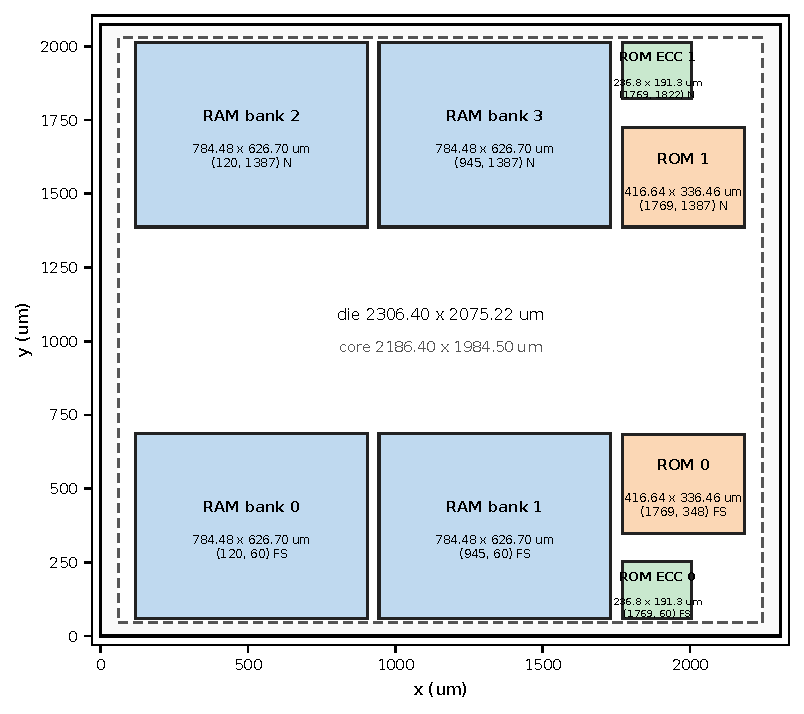
\includegraphics[width=\linewidth]{figures/floorplan_macros.pdf}
  \caption[The floorplan and the eight macros]{The die outline, the core
  area and the eight vendor macros with their sizes, origins and
  orientations, drawn from the sign-off run's own DEF by
  \code{thesis/figures/\allowbreak make\_layout\_figures.py}. Two macro
  rows face a \qty{700.08}{\micro\metre} standard-cell channel; the
  third column carries the boot ROM and, in the height the shorter ROM
  macro leaves over in each row, its two check macros. These eight are
  the only instances on the die whose position a person chose.}
  \label{fig:phys-floorplan}
\end{figure}

The die is $2306.40 \times 2075.22$\,\si{\micro\metre}, reported as
\qty{4786290}{\micro\metre\squared} and exactly
\qty{4786287.408}{\micro\metre\squared} as the product of the DEF's own
\code{DIEAREA} corners (\dcite{59}{section 4.1}). The core runs from
$(60.00,\,45.36)$ to $(2246.40,\,2029.86)$\,\si{\micro\metre}:
$2186.40 \times 1984.50$\,\si{\micro\metre} and
\qty{4338910}{\micro\metre\squared}. Alignment is asserted rather than
arranged --- \num{2186.40} is exactly 4,555 sites of
\qty{0.48}{\micro\metre} and \num{1984.50} exactly 525 rows of
\qty{3.78}{\micro\metre}, and every macro origin is an integer number of
sites and rows from the core's lower left corner
(\dcite{47}{section 6.1}) --- and \code{hw/soc/pnr/floorplan.py} refuses
to emit a floorplan that has lost the property, reading macro
dimensions from the installed PDK's LEF rather than from a transcript.

\begin{table}[tbp]
\centering
\caption{The eight macros, from the run's own \code{resolved.json} and
the vendor LEF \code{SIZE} statements. All eight are \code{FIXED}.}
\label{tab:phys-macros}
\small
\begin{tabular}{@{}llrrl@{}}
\toprule
\textbf{Instance} & \textbf{Master} & \textbf{$W \times H$, \si{\micro\metre}} & \textbf{Origin, \si{\micro\metre}} & \textbf{Orient} \\
\midrule
\code{u\_ram...u\_b0} & \code{2048x64} & $784.48 \times 626.70$ & (120.00,\,60.48) & FS \\
\code{u\_ram...u\_b1} & \code{2048x64} & $784.48 \times 626.70$ & (944.64,\,60.48) & FS \\
\code{u\_ram...u\_b2} & \code{2048x64} & $784.48 \times 626.70$ & (120.00,\,1387.26) & N \\
\code{u\_ram...u\_b3} & \code{2048x64} & $784.48 \times 626.70$ & (944.64,\,1387.26) & N \\
\code{u\_rom...u\_b0} & \code{1024x32} & $416.64 \times 336.46$ & (1769.28,\,347.76) & FS \\
\code{u\_rom...u\_b1} & \code{1024x32} & $416.64 \times 336.46$ & (1769.28,\,1387.26) & N \\
\code{u\_rom...u\_c0} & \code{512x16} & $236.80 \times 191.34$ & (1769.28,\,60.48) & FS \\
\code{u\_rom...u\_c1} & \code{512x16} & $236.80 \times 191.34$ & (1769.28,\,1821.96) & N \\
\bottomrule
\end{tabular}
\end{table}

\Cref{fig:phys-floorplan} and \cref{tab:phys-macros} are the
arrangement, and \textbf{it is forced rather than chosen: the forcing
constraint is pin geometry.} Every \code{RM\_IHPSG13} part puts all of
its signal pins on one edge, at local $y=0$, on Metal2 and Metal3 ---
352 on the $2048\times64$ and 190 on the $1024\times32$
(\dcite{47}{section 6.1}) --- and a macro whose pin edge faces another
macro is a macro the router reaches the long way round. The lower row is
therefore \code{FS}, which mirrors about $X$ and lifts its pins to its
\emph{top}; the upper row is \code{N}, which leaves its pins at its
\emph{bottom}; and both face the \qty{700.08}{\micro\metre} channel
between them. Rotating a hard macro is not an option this project can
check, for the reason \cref{sec:phys-decks} gives.

\textbf{The two ROM check macros fit without growing the die, and why
they sat unplaced for weeks is worth more than the placement.} The open
item read that there was \qty{60.48}{\micro\metre} beside each ROM and
the check part is \num{236.80} wide --- true, and a measurement of the
wrong axis. A macro row is as tall as the RAM,
\qty{626.70}{\micro\metre}; the ROM is \num{336.46}; the third column
therefore carries \qty{290.24}{\micro\metre} of unused height per row
and the check macro is \num{191.34} tall. The real obstacle was pins:
the bottom row is \code{FS}, so its ROM's pins are at its top and a
check macro in the pocket \emph{above} it would sit across every wire
leaving them. The bottom ROM is raised to the top of its own band, to
$y=347.76$, and the check macro takes the blind space beneath;
clearances are \qty{95.94}{\micro\metre} and \qty{98.24}{\micro\metre}
with a \qty{10}{\micro\metre} halo, computed from the LEF size and row
pitch and asserted, never written down as a coordinate
(\dcite{67}{section 11}). The die, the core and the four RAM origins do
not move, which keeps measurements on the earlier six-macro floorplan
comparable with these.

\textbf{The die has named zones, and they are the vocabulary the rest of
this chapter uses}, as \code{hw/soc/pnr/\allowbreak clint\_region.py}
defines them after \dcite{72}{section 6.4}: the \emph{channel} is
$687.18 \le y < 1387.26$; the \emph{upper} and \emph{lower pockets} are
the areas at $x \ge 1769.28$ above each ROM, each including the strip
beside it at that height; the \emph{strip} is $x \ge 2185.92$. One
caveat comes with the definition, because the figures inherit it: those
constants are the six-macro floorplan's, in which the lower ROM sat at
$y=60.48$. Here it is at \num{347.76} with the check macro beneath, so
the zone predicate and the ``lower pocket'' outline in
\cref{fig:phys-density} describe the earlier geometry, and the zone
census quoted below is a measurement on that earlier layout.

\textbf{Forced is not untested.} Two alternatives were hardened --- a
channel of 82 rows instead of 185, and a die \qty{19.8}{\percent}
narrower with the ROMs as islands --- and both are worse at every stage
measured, by \qty{0.84}{\nano\second} and \qty{1.70}{\nano\second} at
post-clock-tree and, for the one that routes, \qty{10.09}{\nano\second}
after global routing on \qty{44.1}{\percent} more wirelength. Shrinking
the die spread the logic rather than compacting it: the tight variant
exiled 7,857 of 27,558 cells into the ROM pockets against 739
(\dcite{48}{sections 4 and 5}).

\section{Where the logic went}

\begin{figure}[tbp]
  \centering
  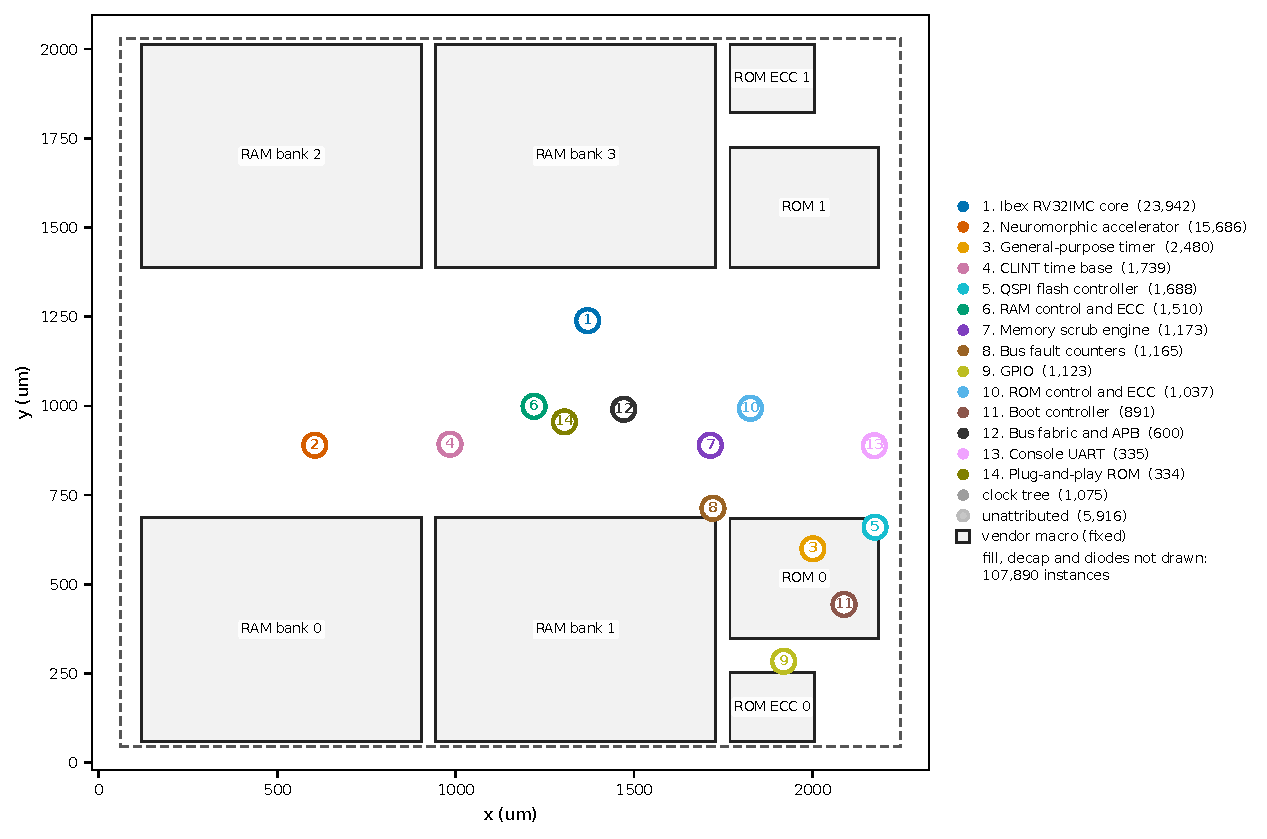
\includegraphics[width=\linewidth]{figures/layout_blocks.pdf}
  \caption[The whole die, coloured by block]{Every standard cell in the
  sign-off layout, coloured by the block it was attributed to, with the
  macros drawn, a numbered centroid per block and per-block counts in
  the legend; the 107,890 fill, decap and diode instances are not drawn.
  Apart from the macros, nothing here was told where to go. The
  attribution method and its \qty{9.75}{\percent} unresolved remainder
  are described in the text; a centroid is a mean and can land on a
  macro, which is why markers 3 and 11 sit inside ROM~0.}
  \label{fig:phys-blocks}
\end{figure}

\Cref{fig:phys-blocks} answers ``where is the processor, where is the
memory'' for a die carrying 168,592 instances, and it must be read with
its method in hand.

\textbf{Exactly one cell on this die could be coloured by its own name.}
Synthesis runs \code{synth -flatten} and then \code{abc}, so of the
168,592 instance names in the DEF only 1,140 carry a dot and 632 of
those are the RAM's; colouring only those would colour a few per cent of
the die and put the processor in the wrong place, because the register
file keeps its name and the arithmetic unit does not. Attribution is
therefore by connectivity, in three passes: Yosys keeps the hierarchical
name of any net it did not create, so every net named after a top-level
instance votes for that block; each anonymous cell takes the block most
of its pins' nets vote for; and cells still unattributed take the
majority block of the cells they share a net with, twice. Clock buffers,
ties, fill and decap are recognised by name or master and form their own
classes (\code{thesis/figures/\allowbreak make\_layout\_figures.py}).

\textbf{The error bar is printed rather than hidden, and it is larger
than the headline figure suggests.} Of the 60,694 non-fill instances,
\code{thesis/figures/\allowbreak layout\_attribution.json} records 1
attributed by its own name, 643 named nets producing 19,790
attributions by vote, 1,075 classified as clock tree, and 5,916 ---
\qty{9.75}{\percent} --- never resolved, drawn grey and counted in the
legend. The remaining 33,912, \qty{55.9}{\percent} of the non-fill
instances, came from the two rounds of neighbour propagation (arithmetic
on that file's own fields). These maps show where the placer put each
block's logic with most of the attribution from the weakest of the three
passes; the per-block counts are an attribution with that error bar on
them, not a census.

\begin{figure}[tbp]
  \centering
  
\includegraphics[width=\linewidth]{figures/layout_panels.pdf}
  \caption[One panel per block]{The nine most populous blocks, each
  against the whole die in grey. The core fills the upper channel and
  reaches into the upper pocket; the accelerator fills the lower channel
  and the left margin; the peripherals cluster at the right, beside and
  below the ROM macros; the RAM's control and error-correcting logic is
  a thin band on both macro rows' pin edges.}
  \label{fig:layout_panels}
\end{figure}

\Cref{fig:layout_panels} separates what \cref{fig:phys-blocks}
interleaves. The core's 23,942 attributed instances take the upper half
of the channel; the accelerator's 15,686 take the lower half and the
left margin. The RAM control and ECC block's 1,510 instances are not a
blob but a thin band along the facing edges of both macro rows --- it is
the logic that fans out to four macros' pins, and the placer put it on
the pins. The CLINT's 1,739 are the tightest cluster on the die, one
compact blob mid-channel, which matters in \cref{sec:phys-clint};
everything with an external interface sits in the third column, in the
pockets and the strip beside the ROMs, about as far from the RAM as the
core box allows.

\begin{table}[tbp]
\centering
\caption{The instance census, from the run's own
\code{final/metrics.json}. Instance utilisation counts standard cells
and macros against the core area; standard-cell utilisation counts
standard cells against the core area less the macros.}
\label{tab:phys-census}
\small
\begin{tabular}{@{}lr@{}}
\toprule
\textbf{Quantity} & \textbf{Value} \\
\midrule
Instances, total & 168{,}592 \\
\quad vendor macros & 8 \\
\quad standard cells, excluding fill & 64{,}349 \\
\quad fill cells & 104{,}235 \\
\quad antenna cells (of which diodes) & 1{,}575 (1{,}258) \\
Sequential cells & 5{,}998 \\
Integrated clock-gating cells & 3 \\
Timing-repair buffers & 13{,}089 \\
\quad inserted for setup / for hold & 369 / 11 \\
Clock buffers / clock inverters & 815 / 309 \\
Standard-cell area, \si{\micro\metre\squared} & 933{,}010 \\
Macro area, \si{\micro\metre\squared} & 2{,}337{,}520 \\
Rows / sites & 1{,}517 / 1{,}003{,}595 \\
Instance utilisation & 0.7538 \\
Standard-cell utilisation & 0.4662 \\
Legalisation displacement, mean / max, \si{\micro\metre} & 0.075 / 20.04 \\
\bottomrule
\end{tabular}
\end{table}

\Cref{tab:phys-census} is the census. The macros are
\qty{48.8}{\percent} of the die area, and the placeable area left inside
the core --- the core less the macros, which is the denominator the
flow's own utilisation metric uses --- is
\qty{2001390}{\micro\metre\squared}, of which the standard cells fill
\qty{46.6}{\percent}. That denominator is generous: on the six-macro
floorplan \dcite{59}{section 11} measured the union of the DEF's
\code{ROW} statements at \qty{7.66}{\percent} less than it, the macro
halos and the site grid taking the difference. The first layout of this
SoC put \qty{396177.6420}{\micro\metre\squared} of cells into
\qty{2092010.95}{\micro\metre\squared} (\dcite{48}{section 4.1}),
\qty{18.9}{\percent}, and
\dcite{47}{section 8.4} named that sparseness as the probable cause of
what layout was costing in timing. It was not: what has since filled the
die is the design.

\begin{figure}[tbp]
  \centering
  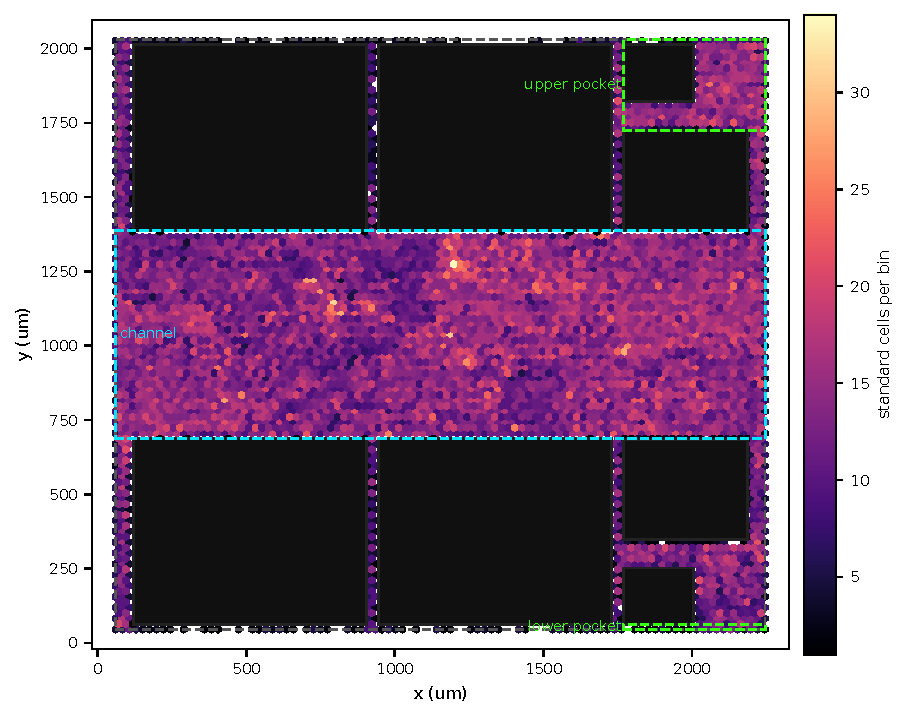
\includegraphics[width=\linewidth]{figures/layout_density.pdf}
  \caption[Standard-cell density over the core]{Hexbin density of the
  non-fill standard cells, macros in black, channel and pocket zones
  outlined. The channel is populated almost uniformly and the rest of
  the logic is in the pockets and the strip at the right. The ``lower
  pocket'' rectangle is drawn from the six-macro floorplan's constants,
  in which the lower ROM sat at $y=60.48$; in this layout the check
  macro stands there, so that outline no longer marks a pocket.}
  \label{fig:phys-density}
\end{figure}

\Cref{fig:phys-density} is the same placement as a density field, and
what it shows is where the logic went: \emph{the channel is not where
all of it is}. That is not what the timing turns on, and the difference
was measured rather than assumed --- on this same run, wire is
\qty{1.9}{\percent} of a violating path at the median and
\qty{3.0}{\percent} at the most wire-bound of 1{,}000, over a median of
78 gate stages, and the CLINT closure the pocket story was about sits
1{,}802 cells of 1{,}802 in the channel with none in either pocket
(\dcite{83}{sections 1, 2 and 3}). The zone census on the six-macro floorplan puts
45,619 standard cells in the channel, 2,222 in the upper pocket, 3,568
in the lower pocket, 441 in the strip and 436 elsewhere, against a
baseline run of the same floorplan at 45,966 / 2,208 / 3,049 / 424 /
173. Those runs differ by 466 cells of netlist, and the extra cells did
not go into the channel --- it holds 347 \emph{fewer}, and the pockets,
the strip and everything outside them 813 more. A net with one pin in
the upper pocket and one in the channel crosses a ROM macro, and 140
nets did so in one run and 134 in the other (\dcite{72}{section 6.4}).

\section{Timing}
\label{sec:phys-timing}

The flow analyses three corners. It names them exactly, and so does
this chapter: \code{nom\_slow\_\allowbreak 1p08V\_125C},
\code{nom\_typ\_\allowbreak 1p20V\_25C} and
\code{nom\_fast\_\allowbreak 1p32V\_m40C}. Sign-off timing is on
extracted parasitics, at a \qty{20}{\nano\second} period, with a
\qty{5}{\percent} derate, \qty{0.25}{\nano\second} of clock uncertainty
and clock-reconvergence pessimism removal. \code{PNR\_CORNERS} is the
typical and slow pair, so the fast corner is not \emph{optimised}
against during the flow --- but all four corner checkers see all three,
which is what \cref{tab:phys-timing} depends on.

\begin{table}[tbp]
\centering
\caption{Sign-off timing of \code{s83romecc5}: three corners, extracted
parasitics, \qty{20}{\nano\second} period (the run's step-49
\code{summary.rpt} and its \code{final/metrics.json}). No frequency is
derived from any of it.}
\label{tab:phys-timing}
\small
\begin{tabular}{@{}lrrrrrr@{}}
\toprule
\textbf{Corner} & \textbf{Setup WS} & \textbf{Vio} & \textbf{Setup TNS} & \textbf{Hold WS} & \textbf{Vio} & \textbf{Slew} \\
 & ns & & ns & ns & & vio \\
\midrule
\code{nom\_slow\_1p08V\_125C} & $-7.5758$ & 3{,}529 & $-14{,}735.65$ & $+0.4261$ & 0 & 533 \\
\code{nom\_typ\_1p20V\_25C}   & $+2.6396$ & 0 & 0 & $+0.1769$ & 0 & 77 \\
\code{nom\_fast\_1p32V\_m40C} & $+8.3630$ & 0 & 0 & $+0.0296$ & 0 & 20 \\
\bottomrule
\end{tabular}
\end{table}

\textbf{Hold is met at all three corners; setup misses at the slow
corner by \qty{7.5758}{\nano\second} on 3,529 endpoints.} There are also
533 max-slew violations at the slow corner and 98 max-cap violations at
the fast, and the flow exits non-zero naming them --- which it does only
because four keys were set before the first run rather than audited
after it (\dcite{47}{section 7}). Shipped,
\code{SETUP\_VIOLATION\_\allowbreak CORNERS} falls through to the PDK's
\code{["*typ*"]}, so setup would have been examined at the typical
corner alone, where this design passes; and the max-cap and max-slew
checkers' step classes override their corner lists to \code{[""]}, which
is truthy, so the list filters to empty, no corner matches, and the step
\emph{warns} instead of failing. All four are \code{["*"]} here. A fifth
key is a type rather than a value: the derate ships as the integer
\num{5} and \code{base.sdc} computes \code{expr 5 / 100} in Tcl, which
is \num{0}, so nothing is derated while the log says otherwise; the
configuration sets \num{5.0}, and \code{resolved.json} cannot audit it
because it flattens the float back --- a trap that has now bitten in
four places (\dcite{72}{section 7.1}).

Two metrics the flow judges with nothing are reported here rather than
left in a file. \code{Checker.\allowbreak WireLength} has no threshold
in either PDK and so warns and skips, on a layout whose longest routed
net is \qty{4292.89}{\micro\metre}. And the Classic flow has no
max-fanout checker at all, on a layout carrying 589 such violations
against a constraint of 10 and a library declaring
\code{default\_max\_fanout : 8}.

\subsection{The worst path}

\code{hw/soc/pnr/\allowbreak violator\_census.py} resolves all 3,529
violating endpoints against the run's own netlist and finds six launch
points behind them. One is the register file's read address bit
\code{raddr\_b\_i[4]}, which launches 2,865 of them and carries
\qty{-13195.08}{\nano\second} of total negative slack. The others are
360 endpoints from a RAM macro's \code{A\_DOUT[31]}, 154 from
\code{raddr\_b\_i[2]}, 101 from the accelerator's axon register, 38 from
a launch point the census cannot resolve to a public name, and 11 from
the CLINT's \code{mtime} codeword register.

The worst is \emph{a register-file read address into the register file's
own error-correcting encoder}, ending at the check bit
\code{g\_rf\_flops[2].\allowbreak g\_chk.rf\_chk\_q[6]} of that file's
single-error-correcting double-error-detecting code. It decomposes into \qty{2.492291}{\nano\second} of launch clock ---
through the core's integrated clock gate, which is in the launch path
--- and a data path of \qty{27.0731}{\nano\second} over \textbf{77
driver stages, of which \qty{26.290}{\nano\second} is cell delay and
\qty{0.7827}{\nano\second} is net delay}, arriving at
\qty{29.565346}{\nano\second} against a required
\qty{21.989546}{\nano\second}, for \qty{-7.575801}{\nano\second} of
slack (step-49 \code{max.rpt}, slow corner). Seventeen of the 77 stages
are \code{sg13g2\_xnor2\_1}, which is the encoder; eighteen are buffers
or inverters, and fifteen of those carry the \code{rebuffer} or
\code{fanout} names the repair steps give what they insert.

\textbf{Two stages cost \qty{5.701}{\nano\second} between them, and why
neither was repaired is a property of the library rather than of the
resizer.} One \code{sg13g2\_nand4\_1} drives \qty{216.9}{\femto\farad}
to a single load for \qty{3.034}{\nano\second} at a
\qty{3.839}{\nano\second} transition; one \code{sg13g2\_xnor2\_1} drives
\qty{283.6}{\femto\farad} for \qty{2.667}{\nano\second} at
\qty{3.627}{\nano\second}. Both loads are \emph{legal}: the slow-corner
Liberty declares \code{default\_max\_\allowbreak capacitance : 0.3} and
both sit under it, so \code{repair\_design} never looks at them, and the
design has no tighter limit because the capacitance constraint is
optional in LibreLane, neither PDK ships a value, and the flow-written
SDC contains no \code{set\_max\_capacitance} at all. Neither cell can be
made larger: \code{nand4}, \code{xnor2}, \code{a22oi}, \code{o21ai},
\code{nand3} and \code{a221oi} ship in \emph{exactly one drive
strength}. Both transitions exceed the library's
\code{default\_max\_\allowbreak transition} of
\qty{2.5074}{\nano\second}, which is what the slow corner's 533 max-slew
violations are. Tightening the capacitance limit was measured to
sign-off on an earlier layout and cost \qty{1.6525}{\nano\second},
because \code{repair\_design} is a global instrument and the problem is
local: it buffered 4,163 nets instead of 127 and left the targeted
repair step 615 gate resizes instead of 1,620
(\dcite{48}{sections 6 and 7}).

\subsection{The macro read return}

The second-largest violating launch group is the memory. The
$2048\times64$ macro's \code{A\_CLK}$\rightarrow$\code{A\_DOUT} arc is
\qty{9.2941}{\nano\second} at the slow corner, and it is a function of
macro \emph{depth}: across the eighteen single-port parts it runs from
\qty{5.2678}{\nano\second} at $512 \times 8$ to
\qty{9.6611}{\nano\second} at $8192 \times 32$ while density improves in
the same direction, a \qty{4.3933}{\nano\second} trade end to end. The part
chosen is the smallest byte-writable 64\,KiB build available, the
denser $8192\times32$ having no per-bit write mask
(\dcite{47}{sections 4.1 and 4.2}).

On this layout the arc launches 360 violating endpoints, worst
\qty{-4.1587}{\nano\second}, with \qty{-864.88}{\nano\second} behind
them. On the earlier six-macro layout the same structure was the
\emph{binding} path, and the report charged \qty{9.5277}{\nano\second}
to the arc and \qty{13.1261}{\nano\second} to the 26 standard-cell
stages after it, of which only \qty{0.2481}{\nano\second} was net delay
(\dcite{48}{section 6.2}, superseded 2026-09-13). The conclusion drawn
there holds here: \emph{the wires are not slow, the wires are heavy} ---
the delay is in cells driving capacitance, not in the metal.

\subsection{Where the resizer stopped}

The flow's two post-global-route optimisation stages default to
\code{False} in LibreLane v3.0.5, and nothing in any report says they
did not run: the only evidence is one flow-log line. On the first layout
of this SoC turning them on was worth \qty{4.30}{\nano\second}
(\dcite{47}{section 8.5}). Both are set here.

\textbf{What the setup resizer then does was instrumented rather than
guessed at} --- on the six-macro boot-hardened layout that preceded this
one, not on \code{s83romecc5}, so the figures below are that layout's.
The step was re-executed on its own saved state with OpenROAD's
\code{repair\_setup} trace on, reproducing the flow's step to the byte
--- 53 metrics, zero differing --- and printing why the loop stopped. No
configured limit bound; what ended it was OpenROAD's own rule abandoning
\code{repair\_timing} when total negative slack fails to improve by the
fix-rate threshold in two consecutive hundred-iteration windows ---
\qty{0.02}{\percent} here, the source's \qty{0.01}{\percent} doubled
once past iteration 1,000. It chased its worst endpoint for 257
iterations, from \qty{-12.260}{\nano\second} to
\qty{-7.990}{\nano\second}; took up nineteen more and reverted every
change on seventeen of them after 51 non-improving passes each; and
ended that phase having visited \textbf{20 of 3,365 endpoints}. A second
phase with a reduced move set visited 156 more and found
\qty{0.146}{\nano\second}. The stage that defeated the first drove
\qty{180}{\femto\farad} from the channel at
$(1911.84,\,1224.72)$ into the pocket at $(1973.76,\,1776.60)$ ---
\qty{62}{\micro\metre} across and \qty{552}{\micro\metre} up, over a
\qty{336}{\micro\metre} macro, at a \qty{4.69}{\nano\second} transition
and \qty{3.73}{\nano\second} on one gate that the resizer did size up,
from \code{nor4\_1} to \code{nor4\_2}, without recovering it
(\dcite{72}{sections 3.2, 6.3 and 7}).

\section{Hold, antennas, and \qty{29.6}{\pico\second}}

Hold is met at every corner and the fast-corner margin is
\qty{+0.0296}{\nano\second}, on a small local path: an unused
intermediate-value register in the core's execute block, through one
inverter and one \code{sg13g2\_a22oi\_1} and back to its own $D$ pin,
arriving at \qty{1.353502}{\nano\second} against a required
\qty{1.323898}{\nano\second} (step-49 \code{min.rpt}, fast corner). The
flow inserted 11 hold buffers in the whole design.
\dcite{50}{section 16} calls this the only layout in the project that
meets hold; several earlier six-macro runs also report zero hold
violations at all three corners in their own \code{final/metrics.json},
so what is scarce here is the margin and not the fact.

\textbf{That \qty{29.6}{\pico\second} is the scarcest quantity on this
die, and two experiments have now been spent against it}
(\cref{sec:phys-rdreg} is the second). The first is the antenna repair. \code{s83romecc5} leaves two antenna violations ---
one net into a RAM macro's \code{A\_ADDR[4]} on Metal3 at
$2.26\times$ the ratio limit, one core net at $1.22\times$ --- out of
538 net and 729 pin violations the default repair had already cleared.
Raising the repair from OpenROAD's default three iterations and
\qty{10}{\percent} margin to eight and \num{25} clears them: run
\code{s83ant} reports zero nets and zero pins. It also inserts 60 more
antenna cells --- 1,635 against 1,575, of which 1,318 against 1,258 are
diodes --- and \textbf{loses hold}: \qty{-0.4351}{\nano\second} on 55
endpoints, 38 of them at the fast corner. That is a bad trade, because a
hold violation is a functional failure at any period where an antenna
violation over a ratio limit is a reliability risk to be argued about.

\textbf{And it is structural rather than tunable.} Run \code{s83ant2}
repeats the repair at five iterations and a \qty{15}{\percent} margin
and lands on \emph{exactly} the same layout: 168,737 instances, the same
1,635 antenna cells, hold \qty{-0.4351}{\nano\second} on the same 55
endpoints, every corner identical to four decimals. Both settings
converge on the same 60 diodes, because the repair stops when it is
clean and the default three iterations had simply stopped early. Those
60 diodes are the price of the last two violations and their load is
what breaks hold; the remaining lever is the resizer's hold margin
rather than the repair's aggression, and nobody has pulled it
(\dcite{67}{section 11}).

\section{Two placement experiments}

\subsection{The CLINT cluster probe}
\label{sec:phys-clint}

\dcite{72}{section 6.4} found both layouts of a pair splitting the
CLINT's 32-bit response register across the upper ROM macro, with the
binding stage a one-drive gate driving a macro-crossing net, and asked
for one probe: put the CLINT's read multiplexer and its response
register on one side of that macro, with \emph{the crossing count on the
worst path} as the metric rather than the slack alone. Both forms of the
probe ran on the same six-macro boot-hardened layout as that section's
resizer trace, not on \code{s83romecc5}.

Deriving the cell set is most of the work, because the design is
flattened before \code{abc} and only net names survive.
\code{clint\_region.py} seeds the set with every cell driving a net
named \code{u\_clint.*} or \code{s\_rdata\_clint[*]}, then takes the
fixpoint of ``a cell belongs if every load of every one of its outputs
already belongs, and no output touches a port or a macro pin''. A plain
backward cone does not work: it runs through the fabric's address
multiplexer, the core's arithmetic unit and the register file's read
multiplexer and returns 4,036 cells, because after \code{abc} that is
one combinational cloud. The exclusive rule gives 743 and stops at the
first net a second block also reads.

Two mechanisms were tried. A placement \emph{region} --- OpenROAD's
\code{dbRegion} and \code{dbGroup}, which no LibreLane key reaches,
written into the flow's own saved database between two steps --- fences
the set into a box in the channel under the ROM and \textbf{does not
route}: the fence takes \qty{38102}{\micro\metre\squared} of placeable
area out of a channel that has none to give, 3,076 cells spread into the
macro gaps, and the global router ends with 420 units of overflow. The flow's own manual-placement key, which moves
the same cells to the same coordinates and holds every other cell at the
baseline's placement, routes and reaches sign-off --- and \textbf{the
crossing count on the register-file read went from 2 to 4, not to 0}.

That failure is the finding. The response registers and the exclusive
part of their multiplexer moved; the decode that selects them and the
\code{mtime} error-correcting decoder did not, because the exclusive
rule does not reach them; so every net between the two halves now
crosses the macro. The worst path moved into the CLINT's time base ---
the codeword register through its decoder and back, four crossings,
three stages over \qty{300}{\femto\farad} --- at
\qty{-13.9924}{\nano\second} at sign-off against
\qty{-9.1085}{\nano\second} for the baseline, with the typical corner
failing for the first time. \textbf{The crossing is a property of where
the cut falls, not of which cells are moved}: the response registers,
the fabric decode that selects them and the time base that feeds them
have to be on one side of the macro together. The probe also exposed a
defect found only after both layouts had used the tool --- the
expression reading macro definitions out of the LEF was unanchored, and
the PDK's property-definitions block also contains the word
\code{MACRO}, so a match starting there swallowed the file's first five
macros. On the corrected tool the rule's answer is 999 cells, and its
union with the block's register-to-register closure --- the set that
captures the whole co-placed cluster --- is 1,830
(\dcite{73}{sections 1, 3, 5 and 7}).

\subsection{The memory read register}
\label{sec:phys-rdreg}

The newest measurement in the project, added 2026-09-15, carries the
sharpest methodological lesson. Registering the macro read return ---
so the standard-cell stages after \code{A\_DOUT} no longer share a
period with the arc --- is a synthesis option, and it had been priced
twice on designs that no longer existed. \dcite{50}{section 16} prices
it on the design that does: one synthesis, one layout of that netlist
through the whole flow with the same configuration and initial state,
against \code{s83romecc5} as the other arm.

\textbf{The mechanism works exactly as predicted.} The macro-read launch
group falls from 360 violating endpoints to 17, its worst slack from
\qty{-4.1587}{\nano\second} to \qty{-2.4798}{\nano\second} and its total
negative slack from \qty{-864.88}{\nano\second} to
\qty{-28.87}{\nano\second}; none of the seventeen survivors is on the
bus at all, and sixteen of them capture into the scrub engine's
counter. The
design's total setup violation improves by \qty{21.9}{\percent}, from
\qty{-14735.65}{\nano\second} to \qty{-11509.24}{\nano\second}, the
largest single-change improvement any layout here has produced.

\textbf{And it does not make the part.} The worst path is unchanged in
kind and \qty{0.1636}{\nano\second} worse in value --- still the
register file's read address into its own encoder, which the read register was never
going to touch, lying between the register file and the peripherals
rather than behind a macro. And \emph{hold at the fast corner goes
negative}: \qty{+0.0296}{\nano\second} becomes
\qty{-0.2961}{\nano\second}. Sixty-one new flip-flops and 683 new
instances, placed by the same tool under the same constraints, spend
\qty{325.7}{\pico\second} of a \qty{29.6}{\pico\second} margin. The
option stays at its default, and the experiment establishes the price of
turning it on with the hold margin as it is today, not a recommendation
to turn it on.

\textbf{The first attempt at that run measured nothing, and it is kept
for that reason.} It was launched with the option set in the environment
and completed all 67 steps --- and placed the \emph{baseline} netlist,
because the runner takes its netlist from \code{SYN\_NETLIST}, which
defaults to the baseline path, and the synthesis knob does not reach it;
a \code{grep} for the option's generate-block name on that run's own
netlist returns zero. Its numbers measure nothing, and the run directory
is left in place with that sentence as its label. Nothing in the flow
said so, because the layout is a perfectly good layout of the netlist it
was given: this is the failure mode the project names \emph{the
measurement was taken on the wrong design}.

\section{Geometric sign-off}
\label{sec:phys-decks}

\textbf{The sign-off run's own configuration gates all four deck
families off}, for a measured reason rather than a schedule. A trial
harden containing one \code{RM\_IHPSG13} macro produced 1,106,478 Magic
DRC error boxes --- every one inside the macro footprint and none
outside --- 2,316 KLayout DRC errors and 359 Netgen LVS errors, and
\dcite{12}{section 8} records that as a \textsc{no-go} on that macro
family for this PDK version, tied to an upstream PDK issue. It is a
property of the PDK, not of this design. The decks were therefore run
separately on the sign-off layout, and all four now have a result on the
eight-macro build (\dcite{67}{section 11}):

\begin{itemize}
\item \textbf{Detailed routing.} 0 DRC errors, 0 disconnected pins, 0
  power-grid violations on either net, 0 illegal overlaps; 62,767 signal
  nets and 2 special nets routed with 486,886 vias, all single-cut, over
  \qty{5746921}{\micro\metre} of wire.
\item \textbf{Netgen LVS.} \emph{Circuits match uniquely}, 263
  symmetries, all seven counters zero --- with the vendor macro a black
  box on both sides, so this signs off the connectivity \emph{into} all
  eight macros' pins and says nothing about their internals. Supplying
  the vendor CDL instead makes the run fail, 64,901 netlist nets against
  63,155 layout nets, for the bus-delimiter and global-name
  disagreement the single-macro trial measured as its 359 errors.
\item \textbf{KLayout DRC.} 11,048 markers, \textbf{0 outside the vendor
  macro hierarchy}, on 204 cells of which all 204 are the macros'
  decoders and internal cells.
\item \textbf{Magic DRC}, macros entering as LEF abstracts: 170 error
  boxes, 20 inside a macro footprint and 150 outside --- and
  \emph{every one of the 150 lies within \qty{0.5}{\micro\metre} of a
  macro edge}, none further and none in open routing area. A LEF
  obstruction blanket is one shape more than \qty{10}{\micro\metre}
  wide, so ordinary routing beside it violates a wide-metal spacing rule
  it would not violate against the macro's real geometry; \code{M3.f}
  alone is 102 of the 150. Four of the twenty inside are the check
  macro's pin rectangles for \code{A\_DOUT[14]} and \code{A\_DOUT[15]},
  the two outputs a $512\times16$ row does not use when it holds two
  words' seven check bits, so nothing is routed to them.
\item \textbf{XOR.} Zero differing shapes, on the antenna-repaired
  layout, 2026-09-14 --- the first XOR result in the project on anything
  carrying the ROM's check macros.
\end{itemize}

\textbf{This is what ``clean where the design drew'' means, and the
phrase is doing precise work.} It does not mean the die is
manufacturable. It means that in every deck run, each marker has been
attributed either to vendor geometry or to the interaction between that
geometry's abstract and the design's routing beside it, and none to a
shape this design's flow drew in open area~\cite{companion_decks}. The
total is not available, because no open deck can check these macros at
the pinned PDK version.
One check that did not run is recorded with the ones that did: the
detailed router skips a cut-enclosure rule the PDK states in a form this
OpenROAD build does not implement --- ten warnings over seven layer
names, identical layer for layer in the hardened and baseline runs --- so
it is the PDK's and every layout has inherited it.

\subsection{What the KLayout deck is objecting to}

Because that deck was named as the possible exit from the
\textsc{no-go}, its 2,316 was examined in full, and two caveats on the
number were found that the report prints nowhere.

\textbf{The headline double-counts by construction.} Two rules,
\code{Sdiod.d} and \code{Sdiod.e}, are evaluated over the same derived
layer and flag the identical 1,022 polygons: intersection 1,022,
symmetric difference 0. On the eight-macro layout the structure recurs
at another scale, 4,464 and 4,464 with exact set equality, so the 11,048
markers are 6,584 distinct shapes. \textbf{And the deep-mode count is a
property of the deck rather than of the layout}: the same deck in flat
mode on the single-macro file returns 122,814 against its 2,316, a
factor of 53.0. Any figure
quoted from it has to name the deck and the mode; normalised, the two
decks are a factor of 4 to 9 apart rather than three orders of
magnitude, and they \emph{corroborate} each other on the
contact-enclosure rule.

\textbf{The scope matters as much as the count.} A deck that fires three
rules could be a deck that looked at three; this one declared
\textbf{173 rule categories in 47 groups} --- M1 to M5, V1 to V4, the
top-metal and MIM rules, the well, active, gate, seal and fill families
--- and evaluated all of them over the whole 113\,MB
layout~\cite{krinke2024}. Three fired, all inside vendor geometry.

\textbf{And the count is a property of the macro's structure rather than
of the memory the design asked for}, which a sweep of all twenty-seven
parts settled: the $1024\times8$, $\times16$ and $\times32$ parts are
identical at 2,672 markers across a fourfold difference in stored bits,
the $256\times16$, $\times32$ and $\times48$ at 2,148, the 64-bit parts
add exactly 206 at three different depths, depth moves the count
monotonically --- the row decoder --- and a second port roughly doubles
it. A design that halves its word width buys no reduction whatever. The
deck swap is therefore not the exit: the deck the flow runs is the PDK's
main set, which its own documentation calls verified and intended for
foundry precheck, and the deck that returns zero~\cite{companion_tmr} is
the extra set, which the same documentation calls not verified or
tested~\cite{ihppdk}. DRC was never the binding constraint anyway --- a
design that passes DRC and fails LVS is not signed off
(\dcite{54}{sections 3 and 7}).

\section{Power}

The sign-off run writes a \code{power.rpt} per corner, and
\dcite{67}{section 11} reads the typical corner's as
\qty{56.41}{\milli\watt} in total; the metrics file's stored split,
rounded here to four significant figures, is \qty{32.78}{\milli\watt}
internal, \qty{23.56}{\milli\watt} switching and
\qty{0.06900}{\milli\watt} leakage. \textbf{That is a flow estimate at a
default activity assumption and must be quoted as one}: the default was
pinned on an earlier layout by reproducing that layout's published
figure to every digit with \code{set\_power\_activity -input -activity
0.1 -duty 0.5}, so it is the power of a design in which every top-level
input and every register output toggles 0.1 times per clock period and
spends half its time at 1 (\dcite{57}{section 2}).

Measured instead at the toggle rates of a real program --- on that
earlier six-macro layout, which does not contain the accelerator at all
(\dcite{57}{section 3.2}), so superseded for this design --- the same
recipe gives \qty{33.890}{\milli\watt} computing and
\qty{5.539}{\milli\watt} waiting at the typical corner, the waiting
window being \qty{57.6}{\percent} of the run (\dcite{57}{section 5.2}).
\dcite{67}{section 11} states plainly that no power number in the corpus
has been re-measured on \code{s83romecc5}.
\textbf{Idle is \qty{16.3}{\percent} of busy, and
the reason is a clock gate that had been in the netlist since the core
was brought up and that no document had ever mentioned.} It is the real
PDK cell, bound deliberately because the core's upstream substitute is a
modelling stand-in, and it covers 2,464 of that design's 3,085
flip-flops; on the measured workload it is open \qty{42.4}{\percent} of
the time, with two clock transitions per cycle when open and 0.0004 when
shut (\dcite{57}{section 4}). The sign-off layout carries three such
cells (\cref{tab:phys-census}) where that one carried one; the second
and third are the subject of \dcite{76}{} and \dcite{77}{}.

By group, at the typical corner and measured activity, busy against idle
in milliwatts: combinational \num{13.880} against \num{1.672};
sequential \num{10.749} against \num{2.414}; the clock tree \num{3.828}
against \num{1.281}; the six macros \num{5.433} against \num{0.173}, a
ratio of $31.4\times$ which is the macros' own enable pin doing what it
exists for (\dcite{57}{section 7.1}). \textbf{The clock tree is the
least gateable thing in the design and the smallest of the four}, and
what it costs to wait is three free-running counters --- 231 flip-flops
carrying \qty{99.98}{\percent} of the idle switching between them.

IR drop is reported as \qty{0.0103}{\volt} worst on the supply net and
\qty{0.0441781}{\volt} on the ground net, which \dcite{67}{section 11}
states as \qty{0.86}{\percent} and \qty{3.68}{\percent}. \textbf{Only
the step's connectivity result is used here}: the supply-location file
is unset, so its voltages have no supply position behind them. What it
catches is an unpowered macro, a real risk in this flow --- the
Metal4-to-TopMetal1 connect in \code{hw/soc/pnr/\allowbreak
pdn\_macro.tcl} is the one file without which the macros have no power
and the flow does not notice for thirty-five steps
(\dcite{47}{sections 2 and 9}).

\section{What is open}

\textbf{Setup does not close} (\cref{sec:phys-timing}):
\qty{-7.5758}{\nano\second} on 3,529
endpoints at the slow corner, launched by the register file's read address
that \dcite{50}{section 16} finds unchanged in kind by the one change
that most improves the total. Four leads have been worked through and
none recovers it --- the hierarchy mode and both post-global-route
stages were banked before the first number existed, two alternative
floorplans are worse and one does not route at all, and the capacitance
constraint was measured to sign-off and costs more than it buys. The one unpriced mechanism left is a hold-repair pass aimed at the fast
corner that would let the read register be turned on. The other, a
registered request phase in the bus fabric, was built and priced on
2026-09-16: it takes the design's maximum combinational depth from 81
levels to 69 and its median from 39 to 20, costs
\qty{24.89}{\percent} of the workload's cycle count and
\qty{7618.97}{\micro\metre\squared}, and does not route --- its layout
\code{s89rr1} stops at global routing with 387 overflowing tiles, 353 of
them on Metal5, against zero for this one (\dcite{84}{sections 1 and
11}).

\textbf{The macros cannot be signed off, and therefore neither can the
die.} Every macro area here is a LEF \code{SIZE} statement and every
macro timing figure a Liberty arc, and both describe a part no open deck
can check at the pinned PDK version.

\textbf{The redundancy is in the netlist and not in the
placement}~\cite{companion_tmr}. Nothing in this flow requests physical
separation between triple-modular replicas and nothing supplies it by
default: on the
frozen pilot's sign-off layout --- the run \dcite{34}{} superseded on
2026-08-31, whose DEF hash is identical to the current frozen one's ---
the median centre-to-centre distance
between corresponding bits of different replicas is
\qty{27.52}{\micro\metre} against \qty{113.47}{\micro\metre} over all
cross-replica pairs, a $4.12\times$ concentration, with 49 of the 9,075
cross-replica pairs abutting, and the same picture appears on this SoC
across three
triplicated structures and two hardens
(\dcite{79}{sections 1.2 to 1.6}). The likely mechanism is wirelength
minimisation to a shared voter; no seed and no objective function was
varied, so it is evidenced and not established. \textbf{And no campaign
has been re-run on this layout}: every fault-injection number in the
project describes an earlier six-macro build.

One citation disagreement belongs here rather than in a footnote.
\dcite{50}{section 16} attributes the antenna-versus-hold trade to
\dcite{79}{}, which is about replica placement and formal equivalence
and contains no antenna or hold measurement; the trade is measured in
\dcite{67}{section 11}, and the metrics quoted above are read directly
from \code{s83romecc5} and \code{s83ant}.

% SPDX-FileCopyrightText: 2026 Hasan Melih Akbulut
% SPDX-License-Identifier: CC-BY-4.0

\chapter{The measurements, together}
\label{ch:results}

The preceding chapters each carried their own numbers. This one puts
them on one page, states what each of them is evidence \emph{of}, and
then reports the four experiments that were run while this document was
being written, because they are the newest measurements in the project
and two of them change what an earlier chapter would otherwise have
said.

\section{The state of the part, on one page}

\Cref{tab:headline} is the whole design in numbers. Every row names the
document that owns the measurement; where a figure has been superseded,
the superseding document is named rather than the figure silently
replaced, which is the rule \dcite{64}{} sets for this project.

\begin{table}[tbp]
\centering
\caption{Headline measurements of the design as of 15 September 2026.
Each row is measured, not estimated, and names its source. The
layout rows are all from the sign-off run \code{s83romecc5}, the only
layout in the project that meets hold at every corner.}
\label{tab:headline}
\small
\begin{tabularx}{\linewidth}{@{}lXr@{}}
\toprule
\textbf{What} & \textbf{Value} & \textbf{Source} \\
\midrule
\multicolumn{3}{@{}l}{\textit{Process and floorplan}}\\
Technology & IHP SG13G2, 130\,nm, open PDK & \code{docs/12} \\
Die & $2306.40 \times 2075.22$\,\si{\micro\metre} & final DEF \\
Core area & $(60.00,\,45.36)$ to $(2246.40,\,2029.86)$\,\si{\micro\metre} & \code{clint\_region.py} \\
Vendor macros & 8: four $2048\times64$ RAM, two $1024\times32$ ROM, two $512\times16$ ROM ECC & \code{docs/79} \\
Instances placed & 168{,}592 & \code{metrics.json} \\
Instance utilisation & 0.7538 (standard cells 0.4662) & \code{metrics.json} \\
Flip-flops & 5{,}998 & final netlist \\
\midrule
\multicolumn{3}{@{}l}{\textit{Timing, three corners, no frequency claimed}}\\
Worst hold slack, \code{nom\_fast\_1p32V\_m40C} & $+0.0296$\,ns & \code{metrics.json} \\
Worst hold slack, \code{nom\_typ\_1p20V\_25C} & $+0.1769$\,ns & \code{metrics.json} \\
Worst hold slack, \code{nom\_slow\_1p08V\_125C} & $+0.4261$\,ns & \code{metrics.json} \\
Worst setup slack, slow corner & $-7.5758$\,ns & \code{metrics.json} \\
Setup TNS, slow corner & $-14{,}735.65$\,ns over 3{,}529 endpoints & \code{violator\_census.py} \\
Dominant violating launch point & the register file's read address & \code{docs/83} \\
Dominant violating capture class & the register file and the rest of Ibex, 2{,}088 of 3{,}529 endpoints & \code{docs/83} \\
\midrule
\multicolumn{3}{@{}l}{\textit{Geometric sign-off}}\\
Route DRC errors & 0 & \code{metrics.json} \\
Antenna violating nets & 2, and clearing them breaks hold & \code{docs/79} \\
LVS & matches uniquely, macros as black boxes & \code{docs/67} \\
XOR & 0 differing shapes & \code{docs/67} \\
\midrule
\multicolumn{3}{@{}l}{\textit{Where the logic sits} (\cref{fig:layout_panels})}\\
Ibex core and its register file & 23{,}942 instances, upper channel & this document \\
Neuromorphic accelerator & 15{,}686 instances, lower channel and left edge & this document \\
Fill, decap and antenna diodes & 107{,}890 instances, not drawn in the maps & this document \\
Cells not attributable by connectivity & 5{,}916, 9.75\,\% of the logic & this document \\
\bottomrule
\end{tabularx}
\end{table}

Two rows deserve emphasis because they are the ones a reader is most
likely to misread.

\textbf{The worst setup slack is negative and that is not a defect
report.} No frequency is claimed for this design
(\dcite{53}{}, \dcite{05}{rule 5}); the constraint the flow was given is
a period, and the slack is measured against it. A negative worst slack
at the slow corner says what period this layout would \emph{not} make
at that corner, and the honest statement of the result is the number
and the corner together, never a megahertz figure derived from either.

\textbf{The hold margin is 29.6\,ps and everything competes for it.}
That single number is the reason three separate experiments in this
project ended the same way: a change with a clearly positive effect of
its own spends more hold margin than the design has. The antenna
repair does it (\dcite{79}{}), and so does the memory read register
(\cref{sec:rdreg-result}). A design that meets hold by 29.6\,ps is a
design in which the next improvement must be paid for out of hold.

\section{Four experiments, 14--15 September 2026}

\subsection{The event engine's invariant, proved over all reachable
states}

\dcite{56}{section 9.4} had named a gap and declined to close it twice:
the largest register-transfer file in the system-on-chip carried no
formal property set, and the one-line invariant on which its event
mechanism rests --- that the strobe presenting an event to a neuron is
exactly the one state of the event-engine state machine, neither
implied by it nor implying it --- was checked by one simulation test
and one textual guard rather than over all reachable states.

It is now a property set, \code{hw/soc/formal/soc\_npu.sby}, and the
invariant holds: bounded model checking to depth 30, $k$-induction at
depth 16, and a cover showing the state is reachable, all pass.

Two details of how it was made to work are worth carrying, because they
are the kind of thing that costs a day and appears in no manual. The
properties are \emph{included into} the module under a formal guard, not
read as a separate compilation unit, so that the state machine's
signals are in scope natively; a hierarchical reference from an outside
wrapper into a generate scope silently declares a fresh free wire
instead, which is how an earlier attempt on a different block produced a
counterexample that the register-transfer code cannot produce. And the
six submodules in the instantiation closure are read \emph{without} the
formal flag, so that their own property includes --- and the
assumptions inside them --- stay out of this model.

\subsection{The register file with its storage and its scrub}

\dcite{63}{section 18} had measured that the register-file consistency
check of the RISC-V formal framework proves to check cycle 18 on the
core with the error-correcting register file substituted and times out
at 21, 23 and 25 under six engines at four hours each. That document
ranked three routes out and took none of them.

Two were taken here, and the result is a clean separation of what is
hard from what is merely large.

Route 2 asks only the register file: a wrapper that writes a word,
waits while the scrub engine walks, and reads it back, with three more
properties for the scrub's coverage, its arbitration against the core
and its silence when no fault is present. Cover passes --- the scrub
visits all 31 architectural registers. Bounded model checking and
$k$-induction do not: four engines, including a bit-level model checker
and an IC3 implementation, sit at step 4 and two of them report
\textsc{timeout} at 10{,}800 seconds. Step 4 is the first cycle at which
the read-back property examines a stored word, so the solver is being
asked to relate eight parity trees at the write encoder to eight at the
read decoder through thirty-two more encoders in the scrub path.

Route 3 removes exactly that. With the codec replaced by a degenerate
stand-in of the same interface, an IC3 engine proves all four
properties \emph{unbounded} in 44 seconds. The codec's own correctness
is a separate theorem that another job in the same directory already
proves, so the composition is sound: a property of the wrapper that
holds for every codec satisfying decode-of-encode-is-identity holds for
the real one.

The abstraction also taught the wrapper's hidden assumptions. The first
stand-in was the identity code, and bounded model checking failed at
step 3 with every read bit inverted. The cause is in the read path's
correction mask, which flips every bit whose syndrome matches its
column of the parity-check matrix: with an all-zero column set and a
zero syndrome, that is every bit. The register file therefore assumes
that every column of its parity-check matrix is non-zero and that the
encoding of the all-zero word is zero --- both true of the real code by
construction, and both now written down where the next person to
abstract this block will find them.

\subsection{The multiply and divide checks, bounded rather than
stopped}
\label{sec:mext-result}

\dcite{63}{section 8.4} reported six instruction checks stopped without
a verdict after 35 to 40 minutes each, and section 11 of the same
document listed a different solver as the first route out. That route
was taken: all six checks were run again on both the stock and the
substituted core under a second bit-blasting solver, each with an
explicit time bound written into the job so that the status the tool
records is its own word.

All twelve report \textsc{timeout} at 7{,}200 seconds. None closes.

The interesting number is not in the checks but in the witnesses. The
same six cover jobs, which the original solver reached in 9 to 73
seconds, take 1{,}388 to 10{,}999 seconds under the new one --- between
roughly twenty and one hundred and fifty times slower --- while still
passing. Whatever eventually closes a sequential multiplier
equivalence, it is not a change of satisfiability back end: two of them
have now been given the problem and the second is worse at both halves
of it.

\subsection{The memory read register, measured on the design that
exists}
\label{sec:rdreg-result}

\dcite{50}{} priced a response register on the memory read path twice,
on two designs that no longer exist, and five later documents each
recorded that the measurement was owed on the design that does. It was
taken: one synthesis with the register enabled, one full layout of that
netlist, one whole-system simulation.

The mechanism works exactly as \dcite{50}{} predicted. The macro read
return stops being a violating launch group: 360 violating endpoints
become 17, their total violation falls from $-864.88$ to $-28.87$\,ns,
and the design's total setup violation improves by 21.9\,\%, the
largest single-change improvement any layout in this project has
produced. The seventeen that remain do not reach the bus at all;
sixteen of them end in the scrub engine's counter.

And it does not make the part. The worst path is unchanged in kind and
0.16\,ns worse in value, because it was never behind a macro: it is the
register file's read address into the register file's own error-correcting
encoder, whose structural answer is not the fabric's at all. The fabric
captures 54 of the 3{,}529 violating endpoints and the time base 138,
against 1{,}224 in the register file (\code{docs/83} section 4). Worse, the 61 new
flip-flops and 683 new instances cost 325.7\,ps of hold margin at the
fast corner, and the design has 29.6\,ps. The register therefore stays
at its default of disabled, and what the experiment establishes is its
price at today's hold margin rather than a recommendation.

\subsection{A run that measured nothing, kept on purpose}

The first attempt at the experiment above completed all 67 flow steps
and produced a layout of the \emph{baseline} netlist. The synthesis
knob was set in the environment; the place-and-route script takes its
netlist from a different variable and had defaulted to the unmodified
one. Nothing in the flow objected, because the layout was a perfectly
good layout of the netlist it was given.

The run directory is kept, labelled, and its numbers are in no table.
It belongs in this chapter because it is the project's most common
failure shape in its purest form: not a wrong measurement, but a
correct measurement of the wrong thing. The countermeasure that would
have caught it in seconds --- count the mechanism in the netlist before
believing the layout --- is the same one the redundancy guards apply,
for the same reason.

% SPDX-FileCopyrightText: 2026 Hasan Melih Akbulut
% SPDX-License-Identifier: CC-BY-4.0

\chapter{What exists, what does not, and what comes next}
\label{ch:conclusion}

\section{What exists}

A radiation-hardened neuromorphic system-on-chip for the IHP SG13G2
130\,nm open process design kit, in register-transfer form and in
layout, built end to end with open tools.

In register-transfer form: a 32-bit RISC-V application core with a
single-error-correcting register file and a scrub engine that walks it;
a spiking accelerator with its event engine, its address-event queues
and its serial attachment to the core; a bus fabric with a real
peripheral bus behind it; a time base, a general-purpose timer and a
three-stage watchdog; memories behind error-correcting codes; a boot
path that is hardened rather than assumed; and triple-modular
redundancy where the design decided it was worth its area.

In layout: a placed and routed die of $2306.40 \times
2075.22$\,\si{\micro\metre} carrying eight vendor memory macros and
168{,}592 instances, with zero routing design-rule errors, a layout
versus schematic comparison that matches uniquely, a zero-difference
geometric comparison against the extracted view, and positive hold
slack at all three corners. Every geometric error the sign-off decks do
report lies inside a vendor macro or within half a micrometre of one:
the design is clean where the design drew.

And, throughout, an instrumentation layer that is part of the result
rather than scaffolding around it: guards that count redundancy in the
netlist because the source cannot be trusted to survive synthesis,
formal property sets that state one-line invariants over all reachable
states, fault-injection campaigns at both register-transfer and gate
level, and a cross-check that asks whether an any-state theorem and a
campaign agree about the same block.

\section{What does not exist, stated plainly}

No silicon of this system-on-chip. A frozen slice of the accelerator
was prepared for a multi-project shuttle and is pinned by hash; the
submission itself is an owner decision with a deadline and a cost, and
nothing in this document should be read as saying the part has been
fabricated.

No frequency. The project adopted a rule early --- report periods,
slacks and corner names, never a megahertz figure --- and has kept it
through every layout. A reader who wants a speed grade will not find
one here, and that is deliberate.

No mesh. The multi-node link that would make this a neuromorphic
\emph{fabric} rather than a single accelerator is specified down to its
24-bit link word and its per-node counters, and no register-transfer
code implements any of it. By the project's own ranking it is the
highest-leverage unbuilt item in the design.

No closed multiplier proof. Six instruction checks in the formal
programme have no verdict on either core, under two solvers, at a
stated bound of two hours each. The absence is bounded and named; it is
not a pass.

No verdict for the register-file consistency check on the substituted
core at its required depth. What exists instead is a stronger statement
about a smaller thing --- the register file and its scrub proved
unbounded with the codec abstracted --- and a located reason for the
original difficulty.

No flight heritage, no qualification campaign, and no claim that any of
the hardening in this design has been validated by irradiation. Every
hardening claim in this document is a claim about a mechanism, its
cost, and what an injected-fault campaign observed in simulation.

\section{The open items, ranked by what they would settle}

\begin{enumerate}
\item \textbf{The mesh link and a second node.} The largest unbuilt
      thing, and the one that changes what the part is rather than how
      well it does what it already does.
\item \textbf{A registered request phase in the fabric.} The
      register-file read into the peripheral space is the dominant
      violating path in every layout this project has produced, and no
      placement experiment has moved it, because it is a structure and
      not a placement. It is the one change that would change the worst
      number in \cref{tab:headline}, and it is unpriced.
\item \textbf{Hold margin as a first-class budget.} Three separate
      improvements have now been refused because they cost more hold
      than the design has. The next layout study worth running is not
      another improvement but a hold-repair pass aimed at the fast
      corner, to find out whether the 29.6\,ps is structural or
      tunable.
\item \textbf{Irradiation.} Everything in \cref{ch:harden} is a
      mechanism with a simulated campaign behind it. The step that
      would turn it into evidence about silicon is a beam, and it is
      not a step this project can take alone.
\item \textbf{The remaining peripherals.} A second serial port, the
      synchronous and two-wire interfaces, and the space-oriented link
      and bus codecs are specified and unbuilt; one of them is now
      unblocked by a bridge that exists and is proved, and none of them
      is on the critical path of anything above.
\end{enumerate}

\section{What this document is}

A record, not a report. Its distinguishing habit is the one stated in
the introduction and applied in every chapter since: a measurement that
is superseded is marked with its date and left standing, because the
history of a number is evidence about the number. A check that did not
finish is reported in the word its tool used. A result whose scope is
narrower than its headline says so in the same paragraph as the
headline. A run that measured the wrong thing is kept and labelled
rather than deleted, because the failure shape is more instructive than
the result would have been.

That habit has a cost --- this document is longer and less quotable
than a datasheet --- and one benefit that seems worth it: everything in
it can be checked, and the places where it is weakest are the places it
says so itself.


\bibliographystyle{plain}
\bibliography{refs}

\end{document}
